\section{Analysis}\label{sc:analysis}
The rnucs-mesh workflow has been verified with two verification problems.
These problems were chosen so that high energy interactions occur.

\subsection{Problem Description}
The first verification problem consists of a single rectangular volume of
dimensions 22 cm x 44 cm x 186 cm filled with mercury. This geometry can be seen
in Figure \ref{fig:VPI}. The second verification problem builds on the first
geometry by adding a second rectangular volume around the mercury volume.
This volume is filled with steel and has dimensions 44 cm x 88 cm x 372 cm.
This second geometry can be seen in Figure \ref{fig:VPII}.
Both verification problems have the \gls{sns} source. This is a proton source
with energy described by a Gaussian distribution centered around 1 GeV.
The source is located in the xy
plane at z = -256.71 cm and the distribution of the the x plane depends on the
y location.
%
\begin{figure}[h!]
	\centering
	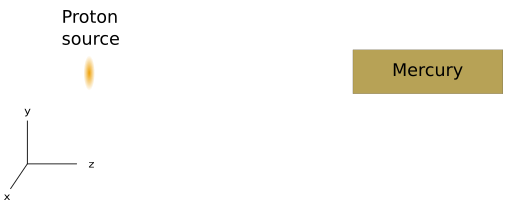
\includegraphics[scale=0.7]{../figs/mercury.png}
	\caption[VPI]{Planar view of Verification Problem I, 22 cm  x 44 cm x 186 cm}
	\label{fig:VPI}
\end{figure}
%
\begin{figure}[h!]
	\centering
	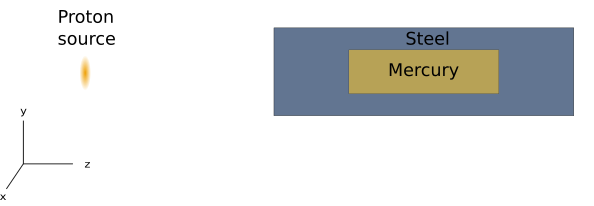
\includegraphics[scale=0.71]{../figs/mer_steel.png}
	\caption[VPI]{Planar view of Verification Problem II geometry, 44 cm x 88 cm x 372 cm}
	\label{fig:VPII}
\end{figure}
%
\subsection{Shut Down Dose Rate Workflow}
The patched \gls{dag}-\gls{mcnp}6 was used to
perform the neutron transport. The neutron flux and the radionuclide information
were collected on a cell, a 1x1x1 mesh, a 2x2x2 mesh, and a 4x4x4 mesh. All
meshes were uniformly distributed Cartesian meshes. In addition, each geometry
was divided into 8 and 64 equal parts. Dividing up the geometry allowed for direct
comparison to the mesh. It is important to note that Verification problem II
required materials to be mixed when the geometry was divided into 8 equal parts as
the division does not align with the cells in the original problem.
Next, an activation script was used to search and write the flux and radionuclide
information for each mesh voxel and geometric cell. A material file was also
written for each region. The script called CINDER90 and a CINDER90 run was
executed for each region.
The photon source script was then used to collect output from CINDER90 to
build a photon source file which can be used in lieu of a source card in the
photon transport. The geometry used for the photon transport was the original
version with a superimposed Cartesian mesh. The photon flux was tallied and
folded with flux-to-dose conversion factors to obtain the biological dose rate
in the mesh.
%
\subsection{Results}
\subsubsection{Verification Problem I}
The radionuclide tally collected information on production and destruction of
isotopes during the neutron transport step. This information was collected
in the mercury volume, using the original rnucs workflow; in each of the previously
mentioned meshes, using the new rnucs-mesh workflow; and on each
volumetric cell of the subdivided geometry, using the original rnucs
workflow.\\
Figure \ref{fig:1prod_cell_1x_2x_4x} shows the radionuclide production information
collected in the mercury volume, the 1x1x1 mesh, and the sum of the results in
each voxel for the 2x2x2 and 4x4x4 meshes. The bottom graph in Figure
\ref{fig:1prod_cell_1x_2x_4x} shows the relative change between each mesh and the
mercury volume.
The relative change between the information collected in a Cartesian mesh and a cell
covering the same phase space is low or none. In this case there are a few isotopes that
have a bigger relative change, but even these isotopes are not statistically different.
%
\begin{figure}[H]
	\centering
	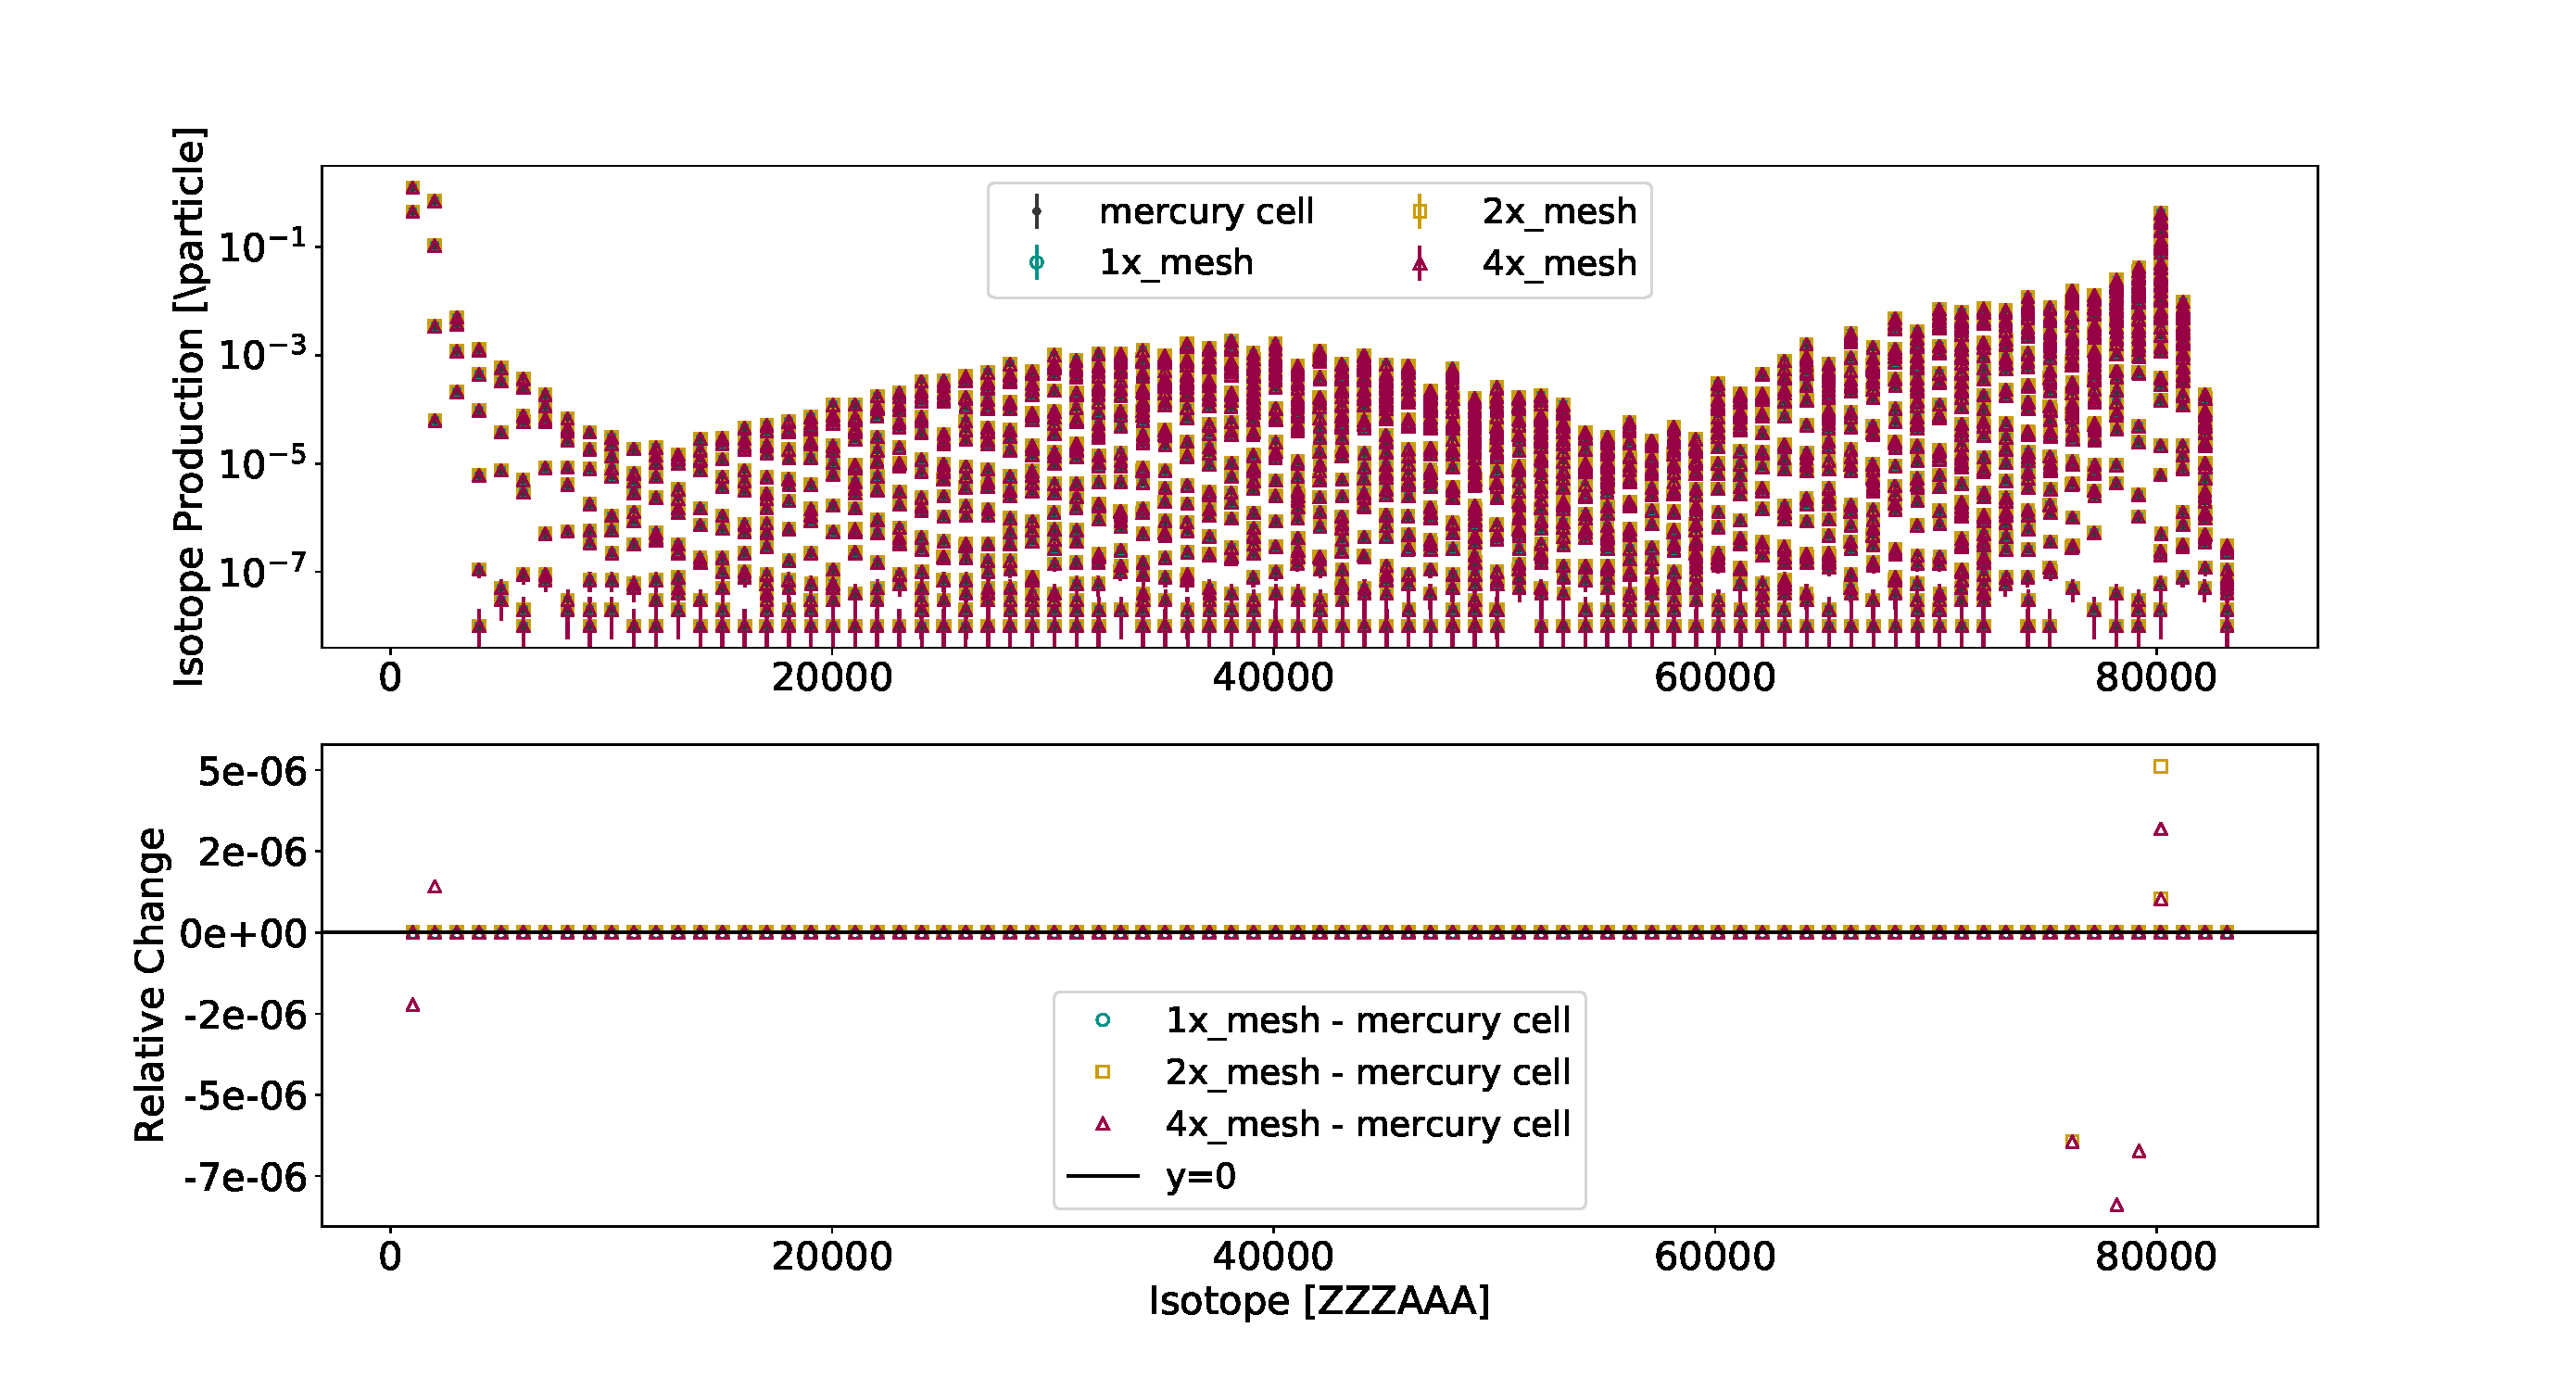
\includegraphics[scale=0.42,trim={2cm 1cm 3cm 2cm},clip]{../figs/toy_p1/prod_VPI_1x_2x_4x.pdf}
	\caption{Radionuclide production comparison for mercury cell and different meshes}
	\label{fig:1prod_cell_1x_2x_4x}
\end{figure}
%
Figure \ref{fig:1prod_cell_2x} compares the results collected in the geometric
cell, the summed up results of a 2x2x2 mesh and the 2x2x2 divided geometry. In
this graph, the relative change for certain isotopes is significantly large.
In order to access this, the absolute
relative change between the divided geometry and the 2x2x2 mesh was compared
to the isotope production results obtained in the mercury volume.
Figure \ref{fig:1prod_cell_2x_rc} shows the relative change is large when the
isotope production per particle is low. This is important to note since these
low production isotopes might be less important to the photon source.
%
\begin{figure}[H]
	\centering
	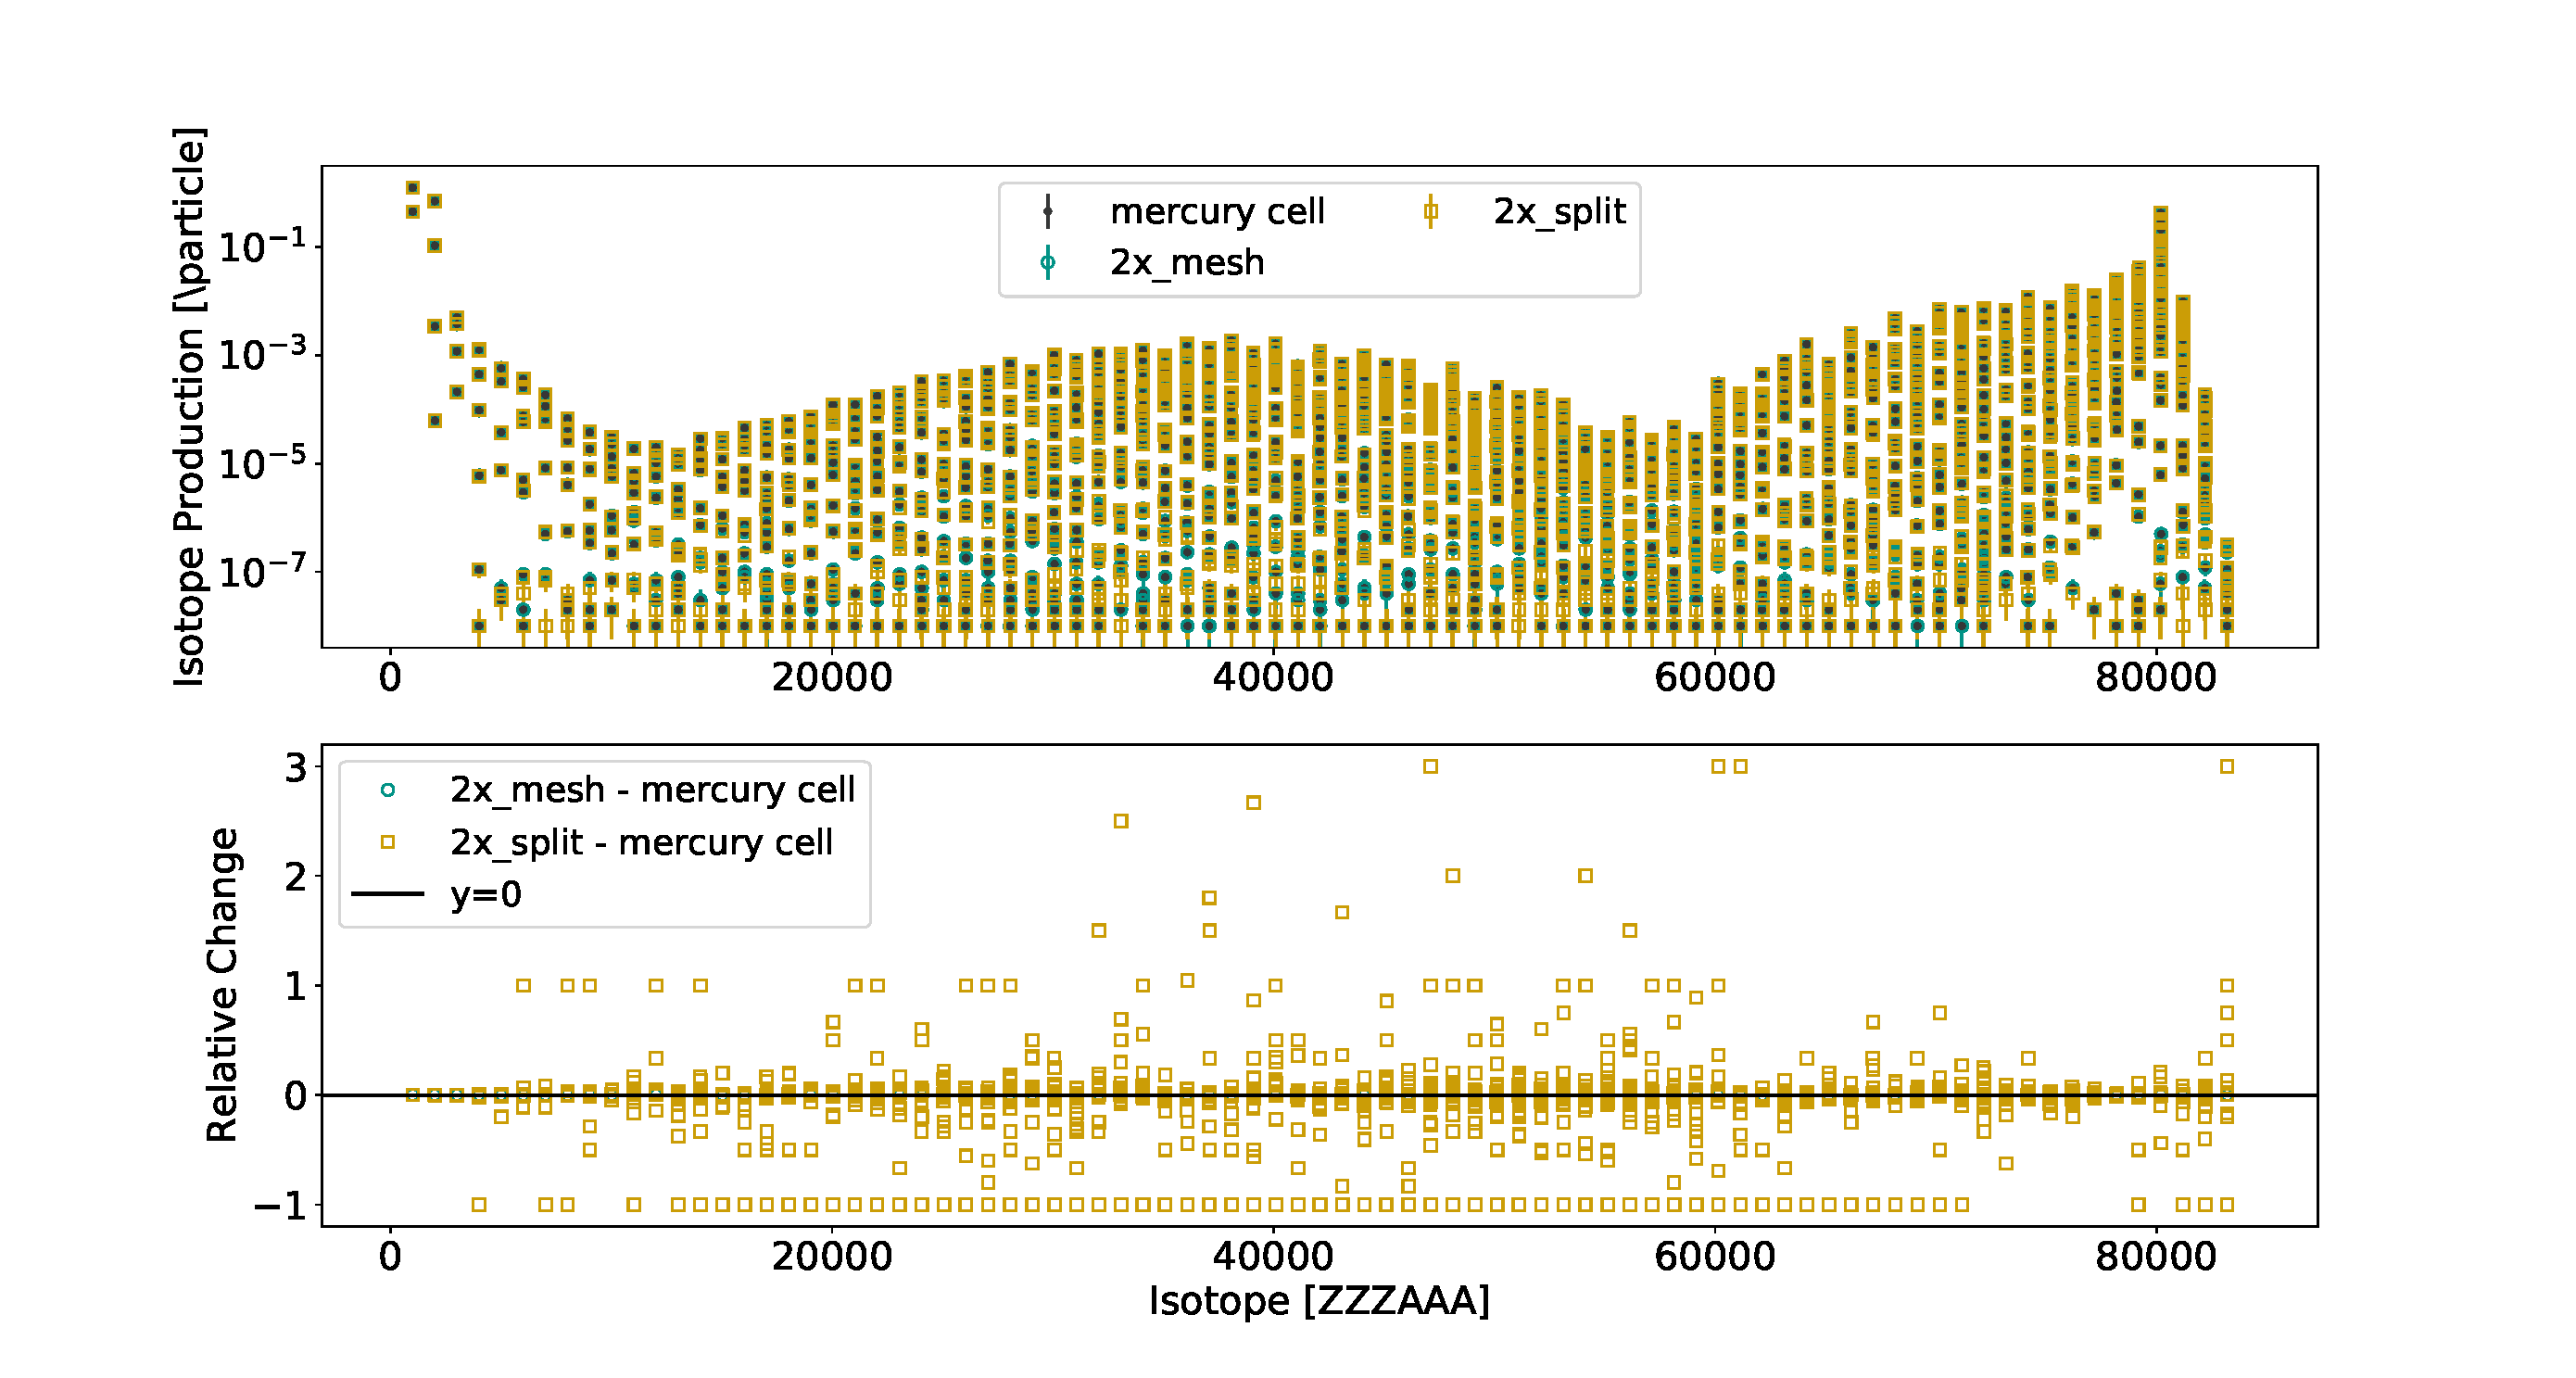
\includegraphics[scale=0.42,trim={2cm 1cm 3cm 2cm},clip]{../figs/toy_p1/prod_VPI_2x.pdf}
	\caption{Radionuclide production comparison between mercury cell, 2x2x2 mesh and geometry split}
	\label{fig:1prod_cell_2x}
\end{figure}
%
\begin{figure}[H]
 \centering
 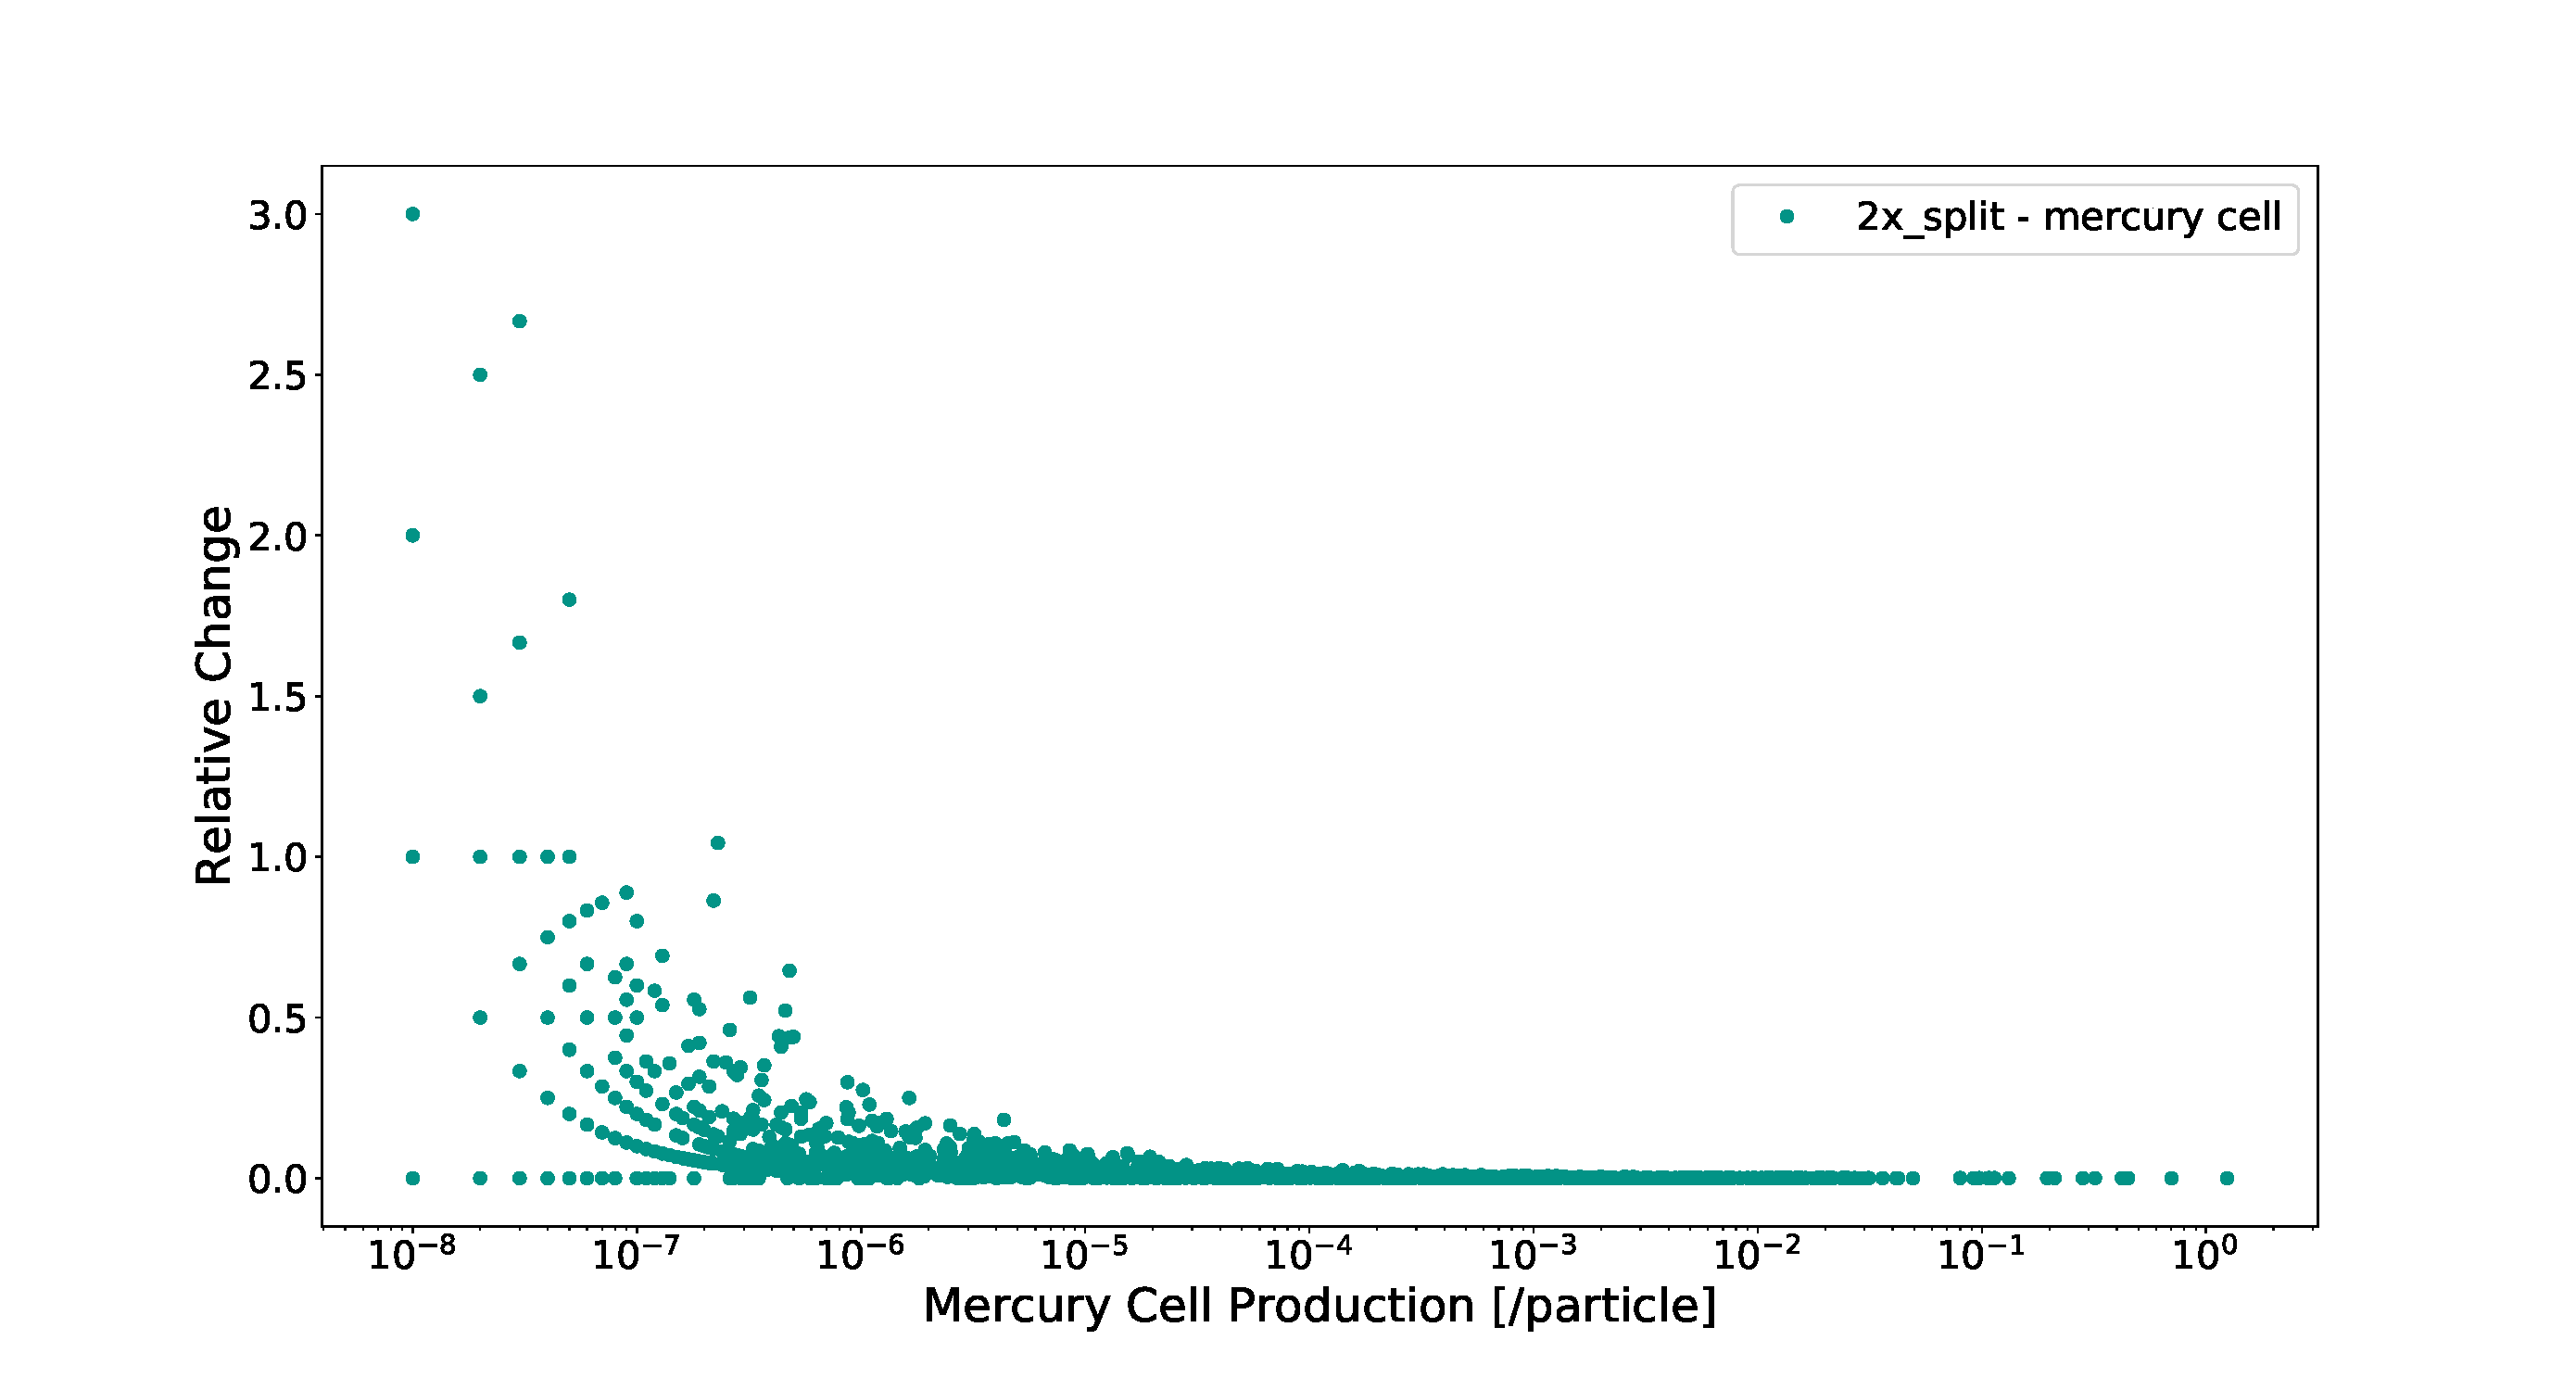
\includegraphics[scale=0.4,trim={3cm 0.5cm 3cm 3cm},clip]{../figs/toy_p1/prod_VPI_rc_2x_split.pdf}
 \caption{Relative change between mercury cell and 2x2x2 geometry split vs. the isotope production of the mercury cell}
 \label{fig:1prod_cell_2x_rc}
\end{figure}

A similar comparison can be seen for the 4x4x4 mesh and the 4x4x4 divided geometry
in Figure \ref{fig:1prod_cell_4x}. The behavior of the relative change is similar
to that of the 2x2x2 divided geometry. A graph comparing the relative change between
the divided geometry and the 4x4x4 mesh  to the isotope production results obtained
in the mercury volume can be seen in Figure \ref{fig:1prod_cell_4x_rc}
%
\begin{figure}[H]
	\centering
	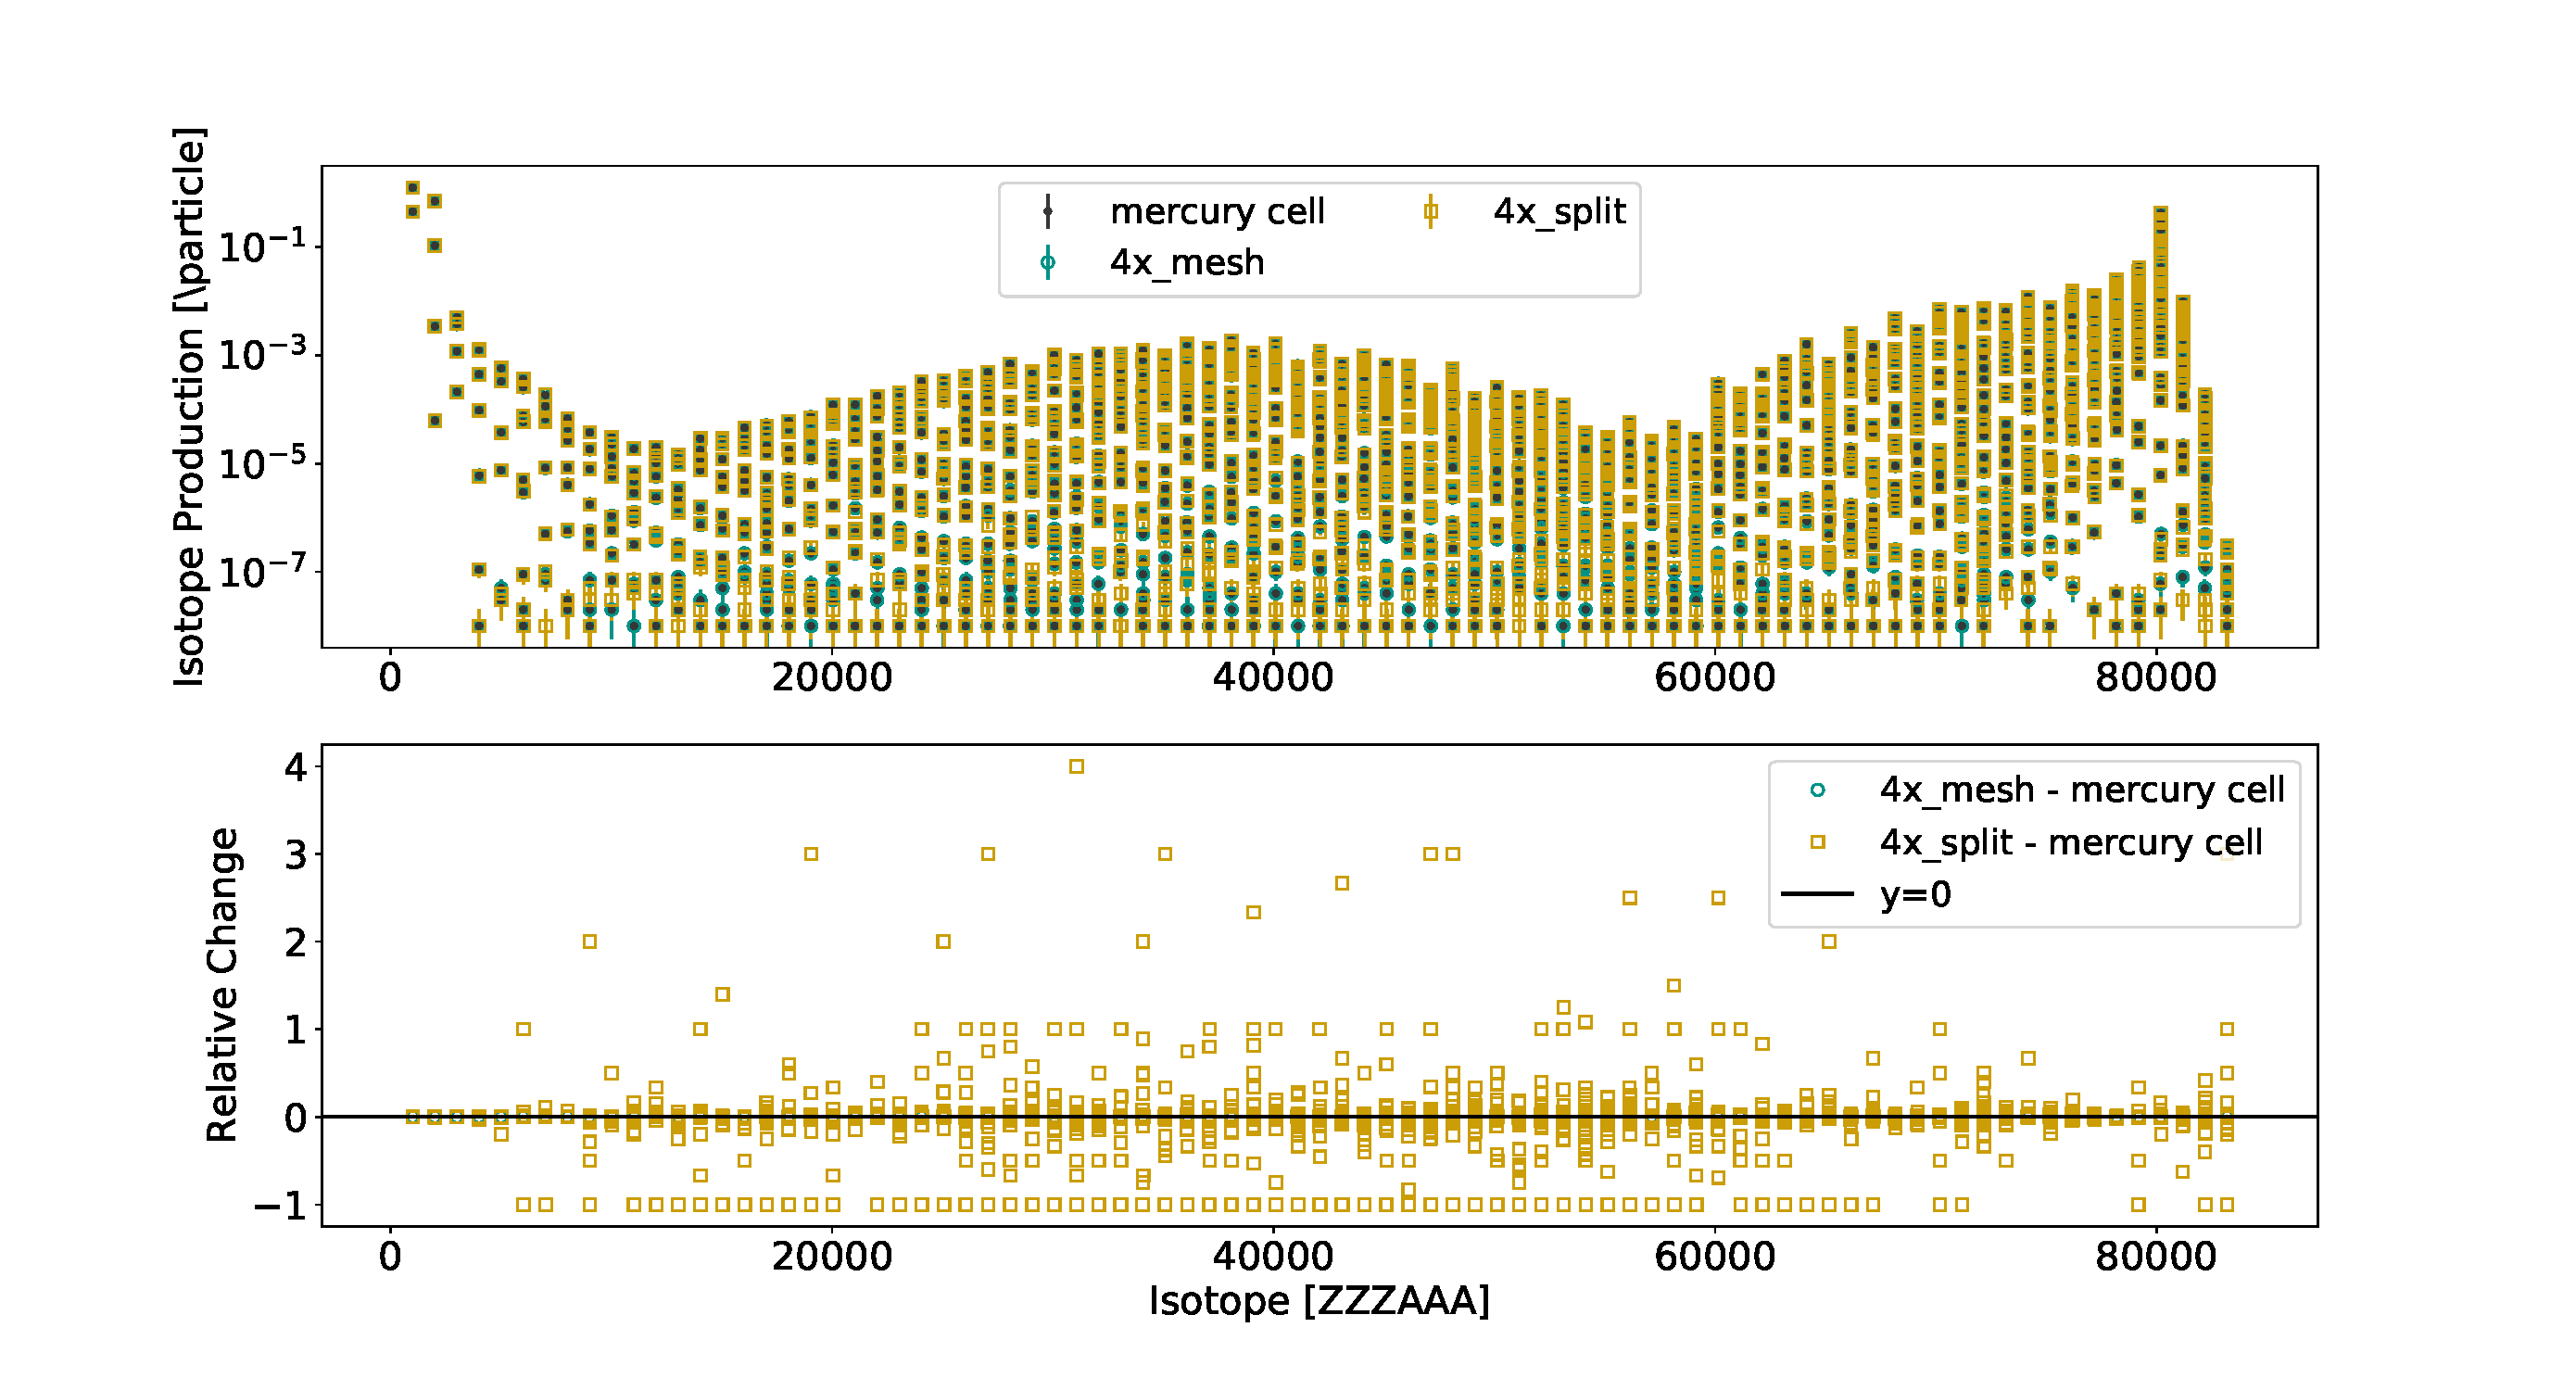
\includegraphics[scale=0.42,trim={2cm 1cm 3cm 2cm},clip]{../figs/toy_p1/prod_VPI_4x.pdf}
	\caption{Radionuclide production comparison between mercury cell, 4x4x4 mesh and geometry split}
	\label{fig:1prod_cell_4x}
\end{figure}
%
\begin{figure}[H]
 \centering
 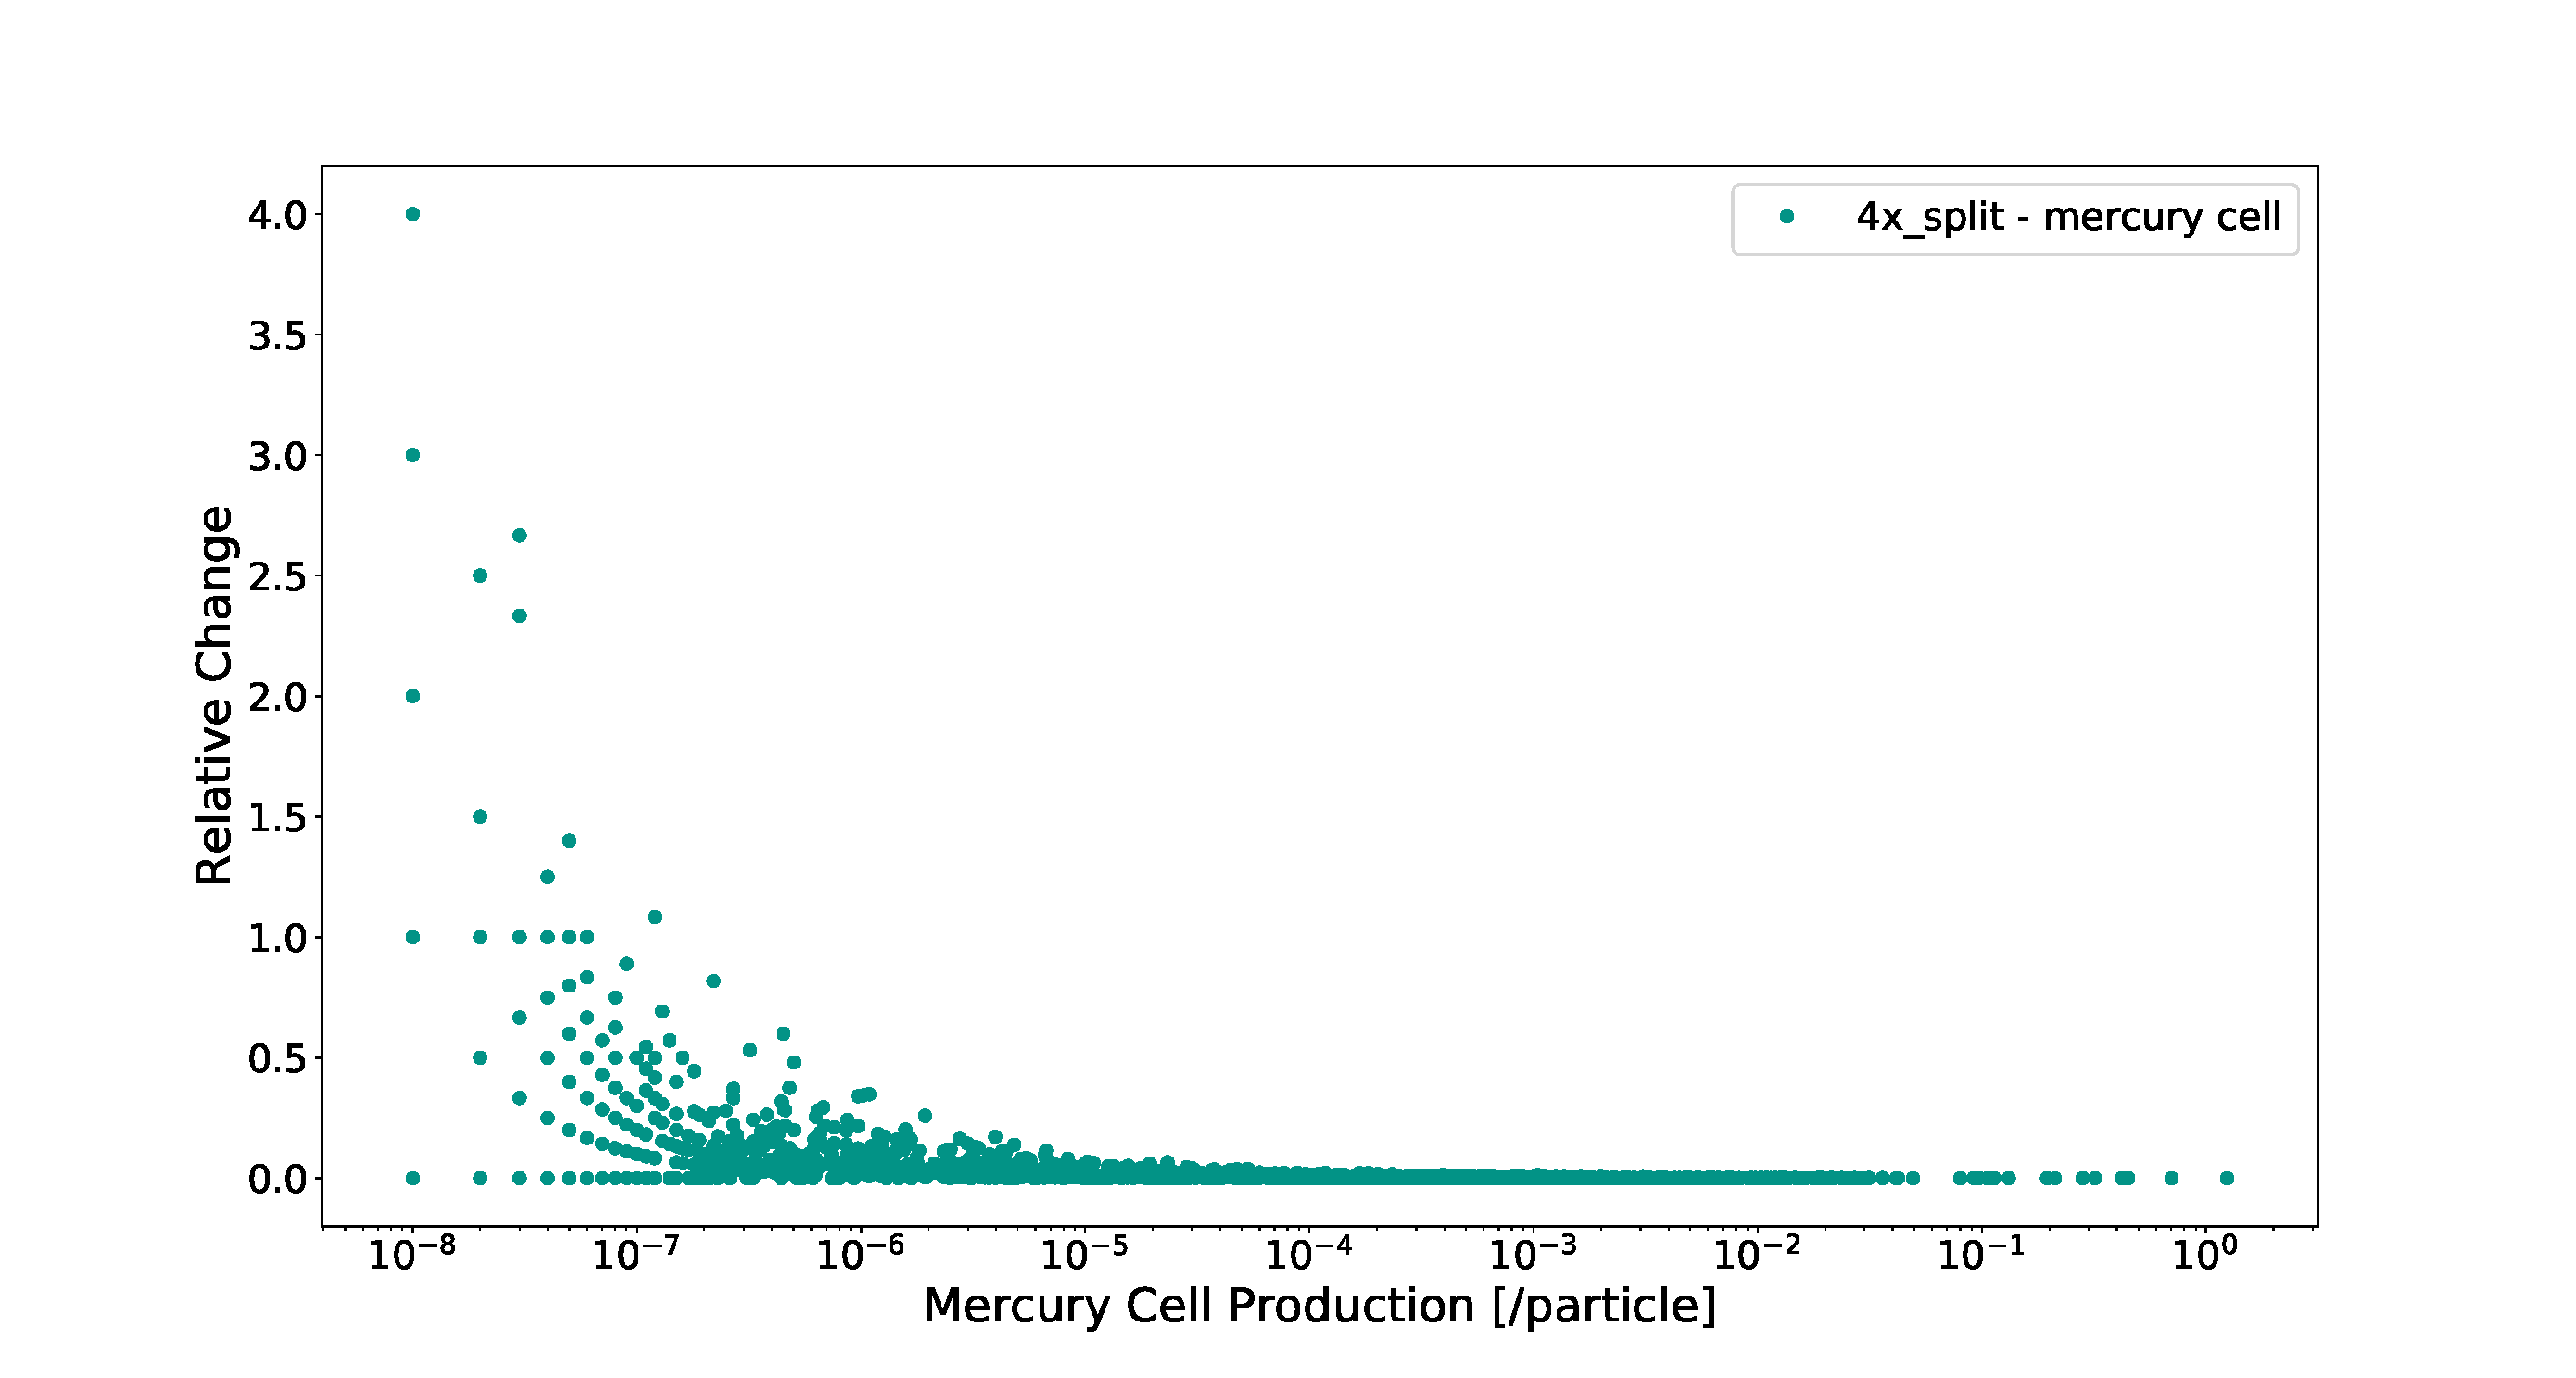
\includegraphics[scale=0.4,trim={3cm 0.5cm 3cm 3cm},clip]{../figs/toy_p1/prod_VPI_rc_4x_split.pdf}
 \caption{Relative change between mercury cell and 4x4x4 geometry split vs. the isotope production of the mercury cell}
 \label{fig:1prod_cell_4x_rc}
\end{figure}
%
For the activation step of the workflow, the photon emission density was collected.
an activation calculation was run for
each problem. The results obtained with information collected in the mercury
cell were compared to results collected in the different meshes and can be seen
in Figure \ref{fig:1spec_cell_1x_2x_4x}. Results were average between all voxels
in a mesh to be able to compare directly to the cell results.
%
\begin{figure}[H]
 \centering
 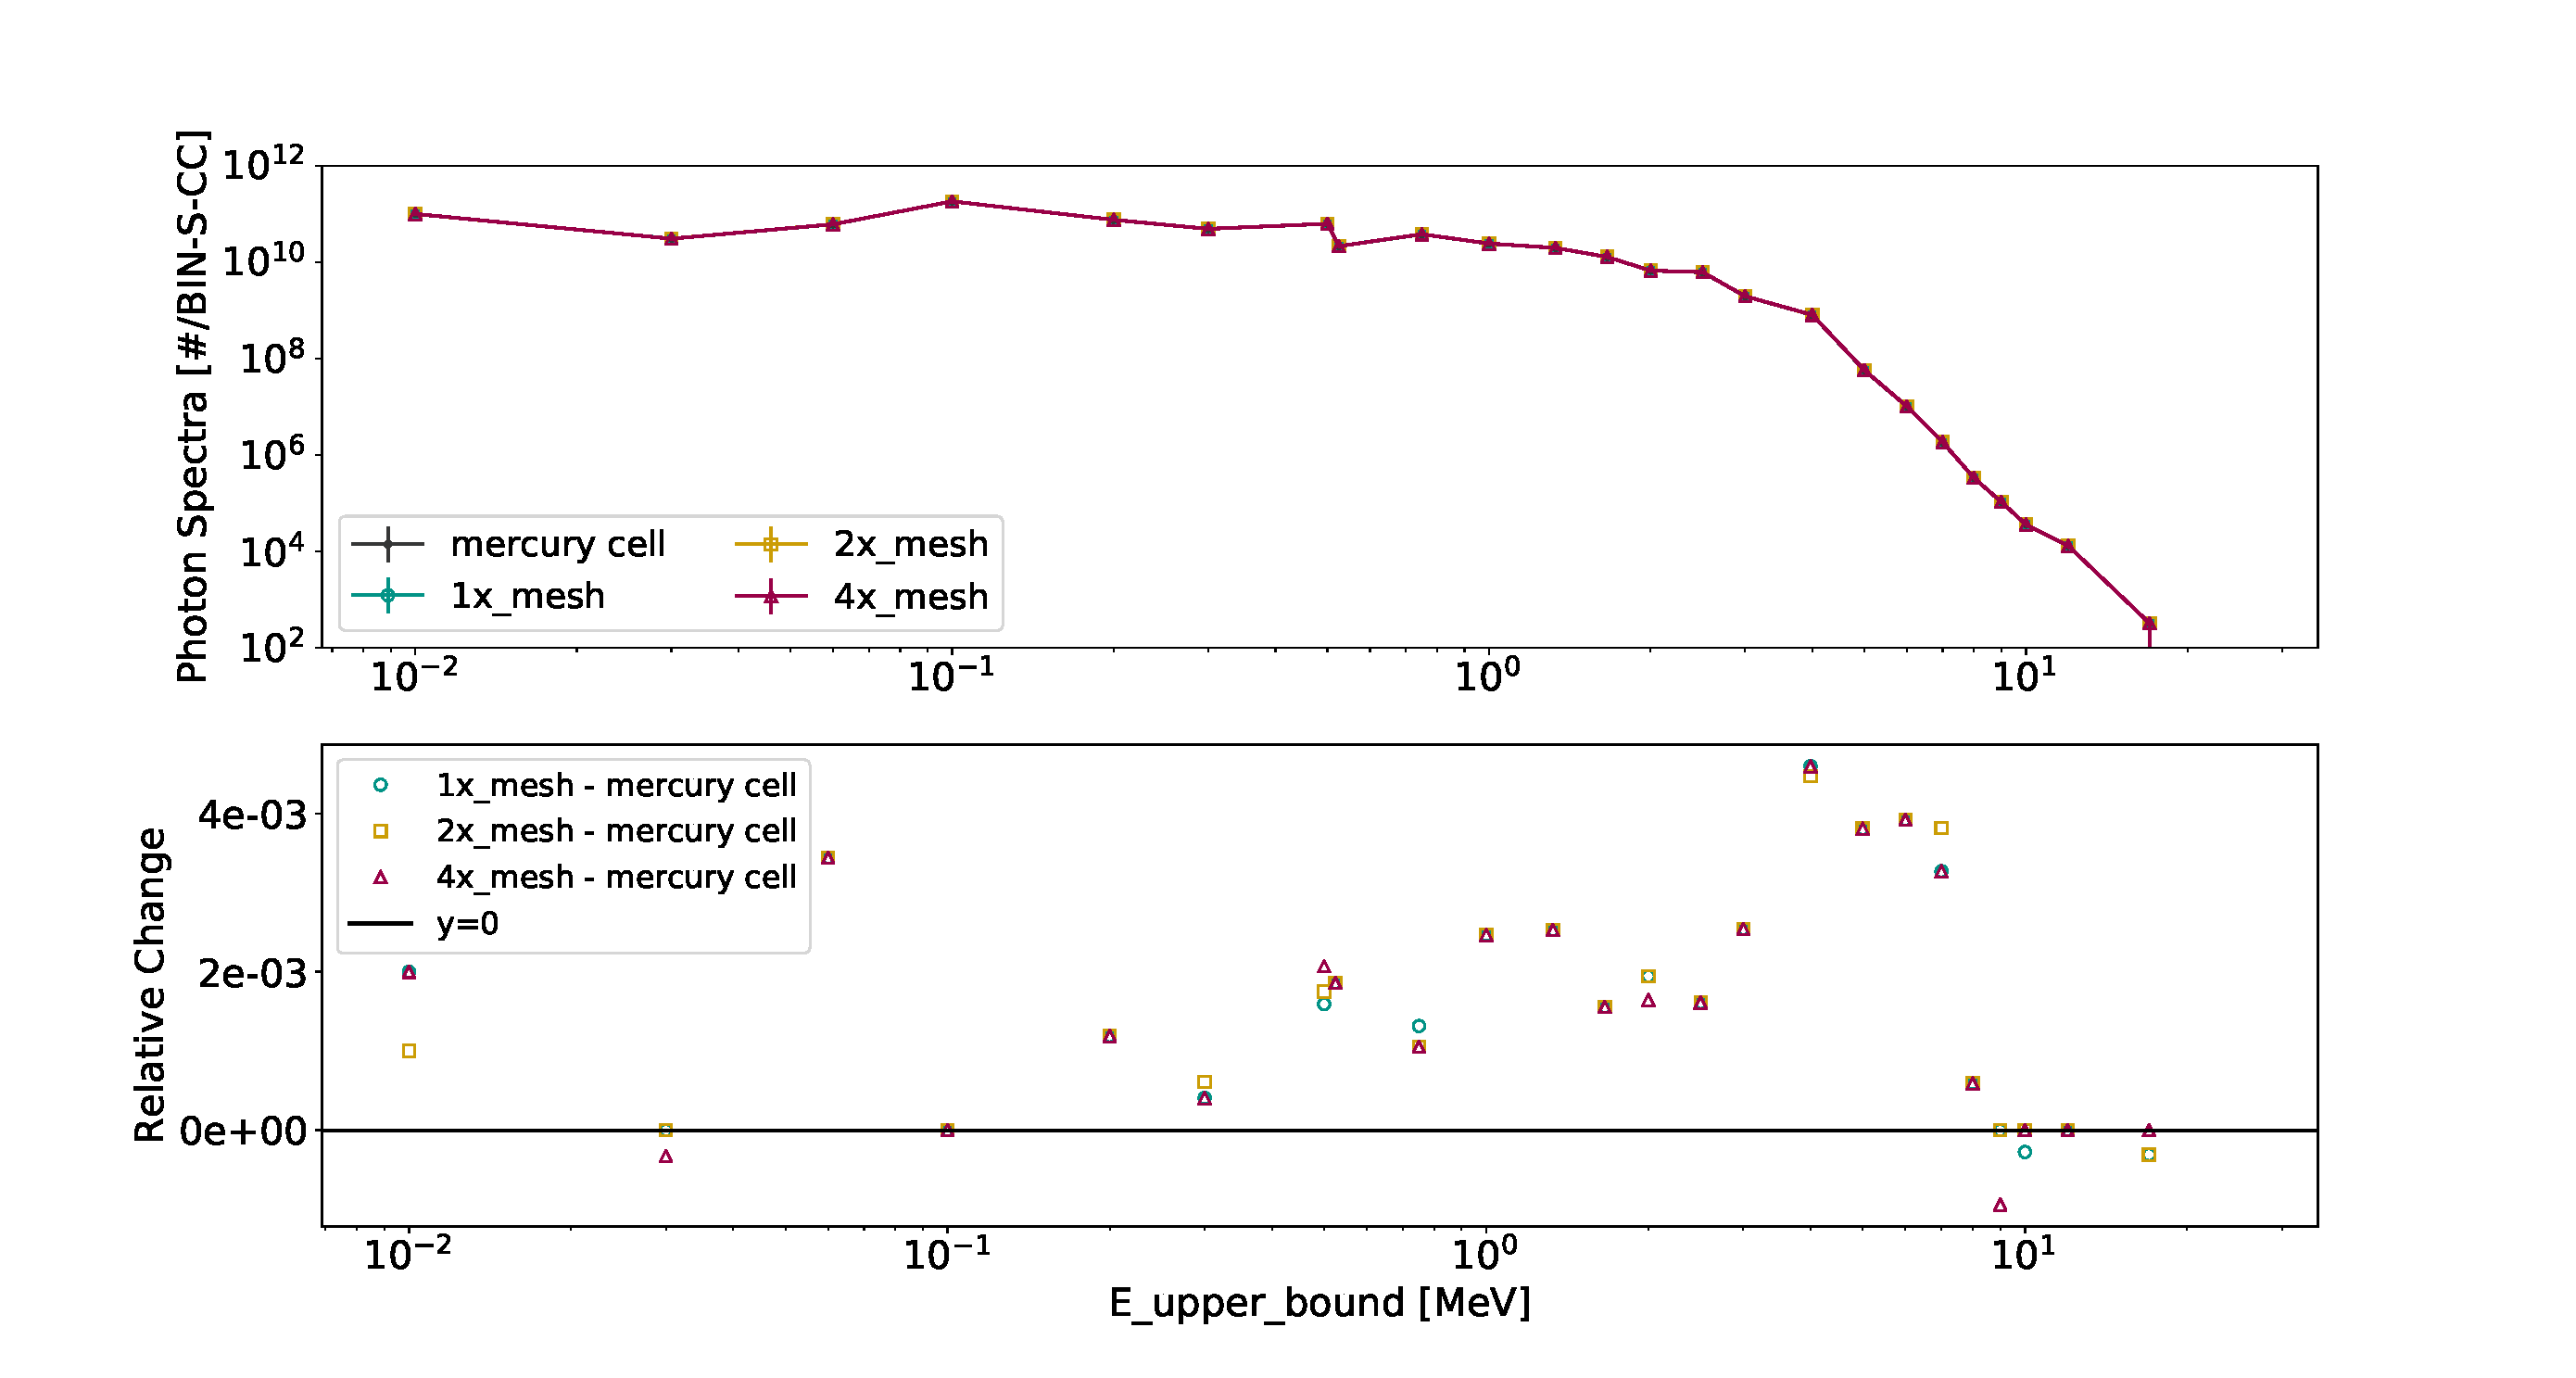
\includegraphics[scale=0.42,trim={2cm 0.5cm 3cm 2cm},clip]{../figs/toy_p1/spec_VPI_1x_2x_4x.pdf}
 \caption{Photon Spectrum in mercury cell and different meshes}
 \label{fig:1spec_cell_1x_2x_4x}
\end{figure}
%
A comparison between the results in the mesh and the split geometry can be seen
in Figure \ref{fig:1spec_cell_2x} and \ref{fig:1spec_cell_4x}.
%
\begin{figure}[H]
 \centering
 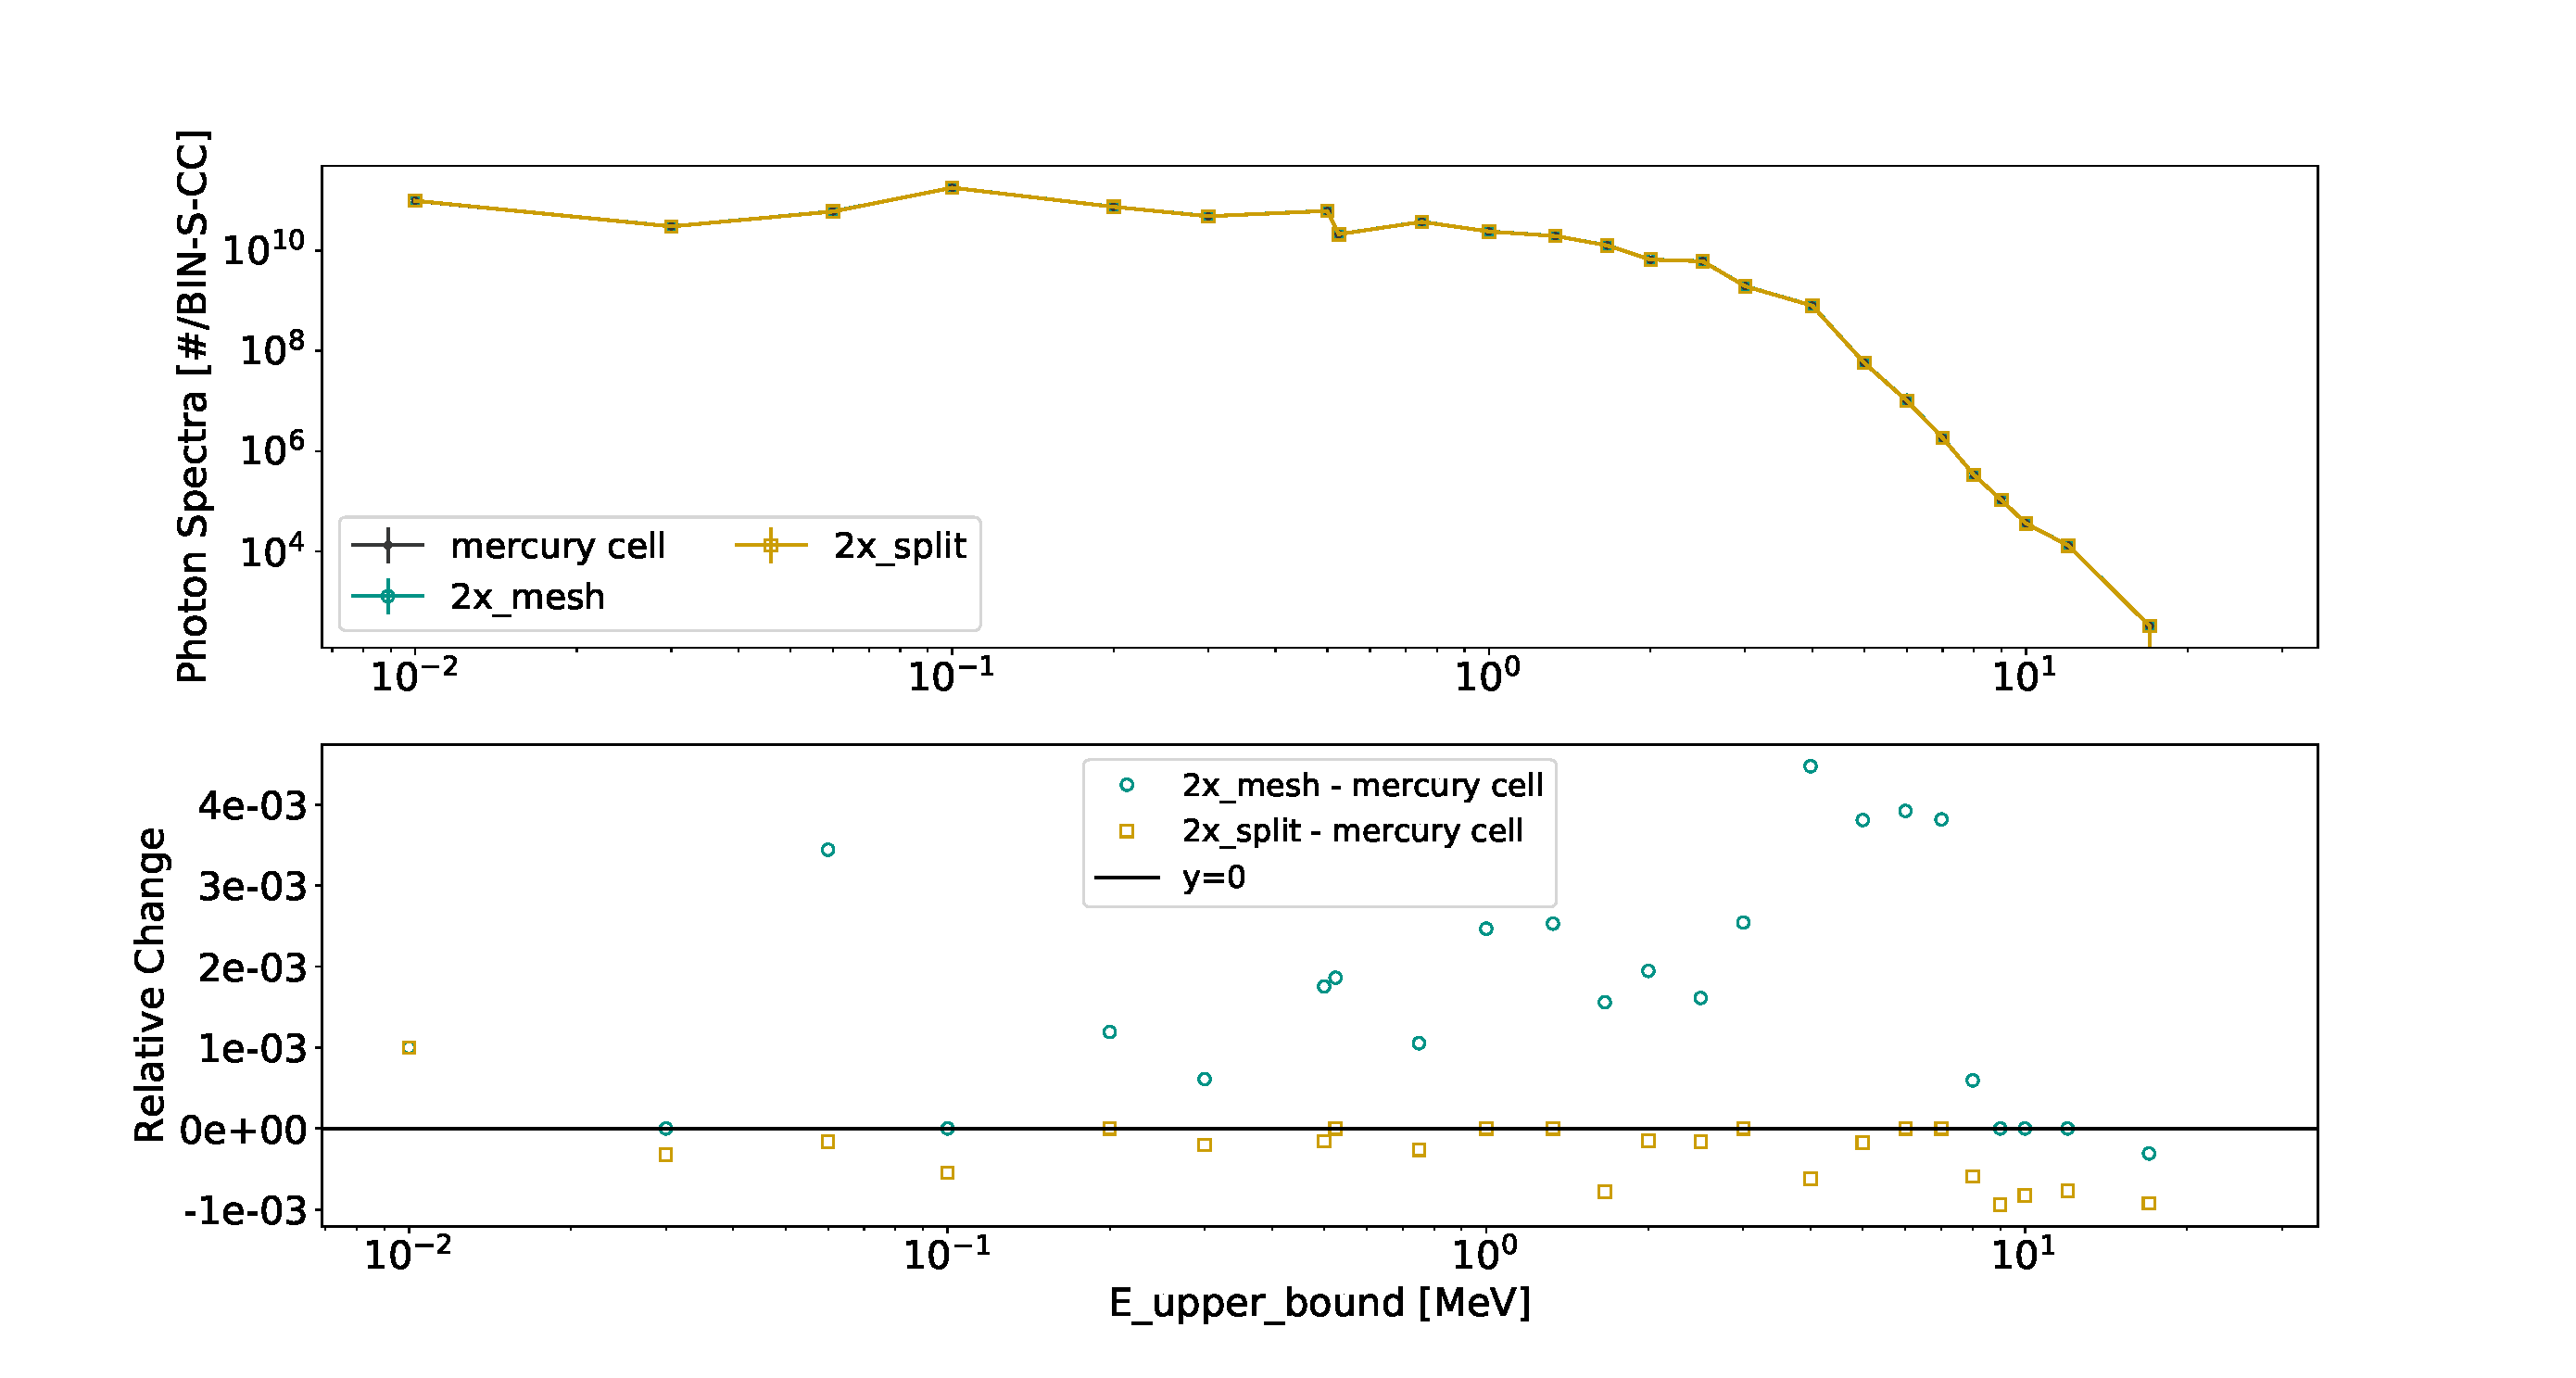
\includegraphics[scale=0.42,trim={2cm 0.5cm 3cm 2cm},clip]{../figs/toy_p1/spec_VPI_2x.pdf}
 \caption{Photon Spectrum in mercury cell, 2x2x2 mesh, and geometry split}
 \label{fig:1spec_cell_2x}
\end{figure}
\begin{figure}[h!]
 \centering
 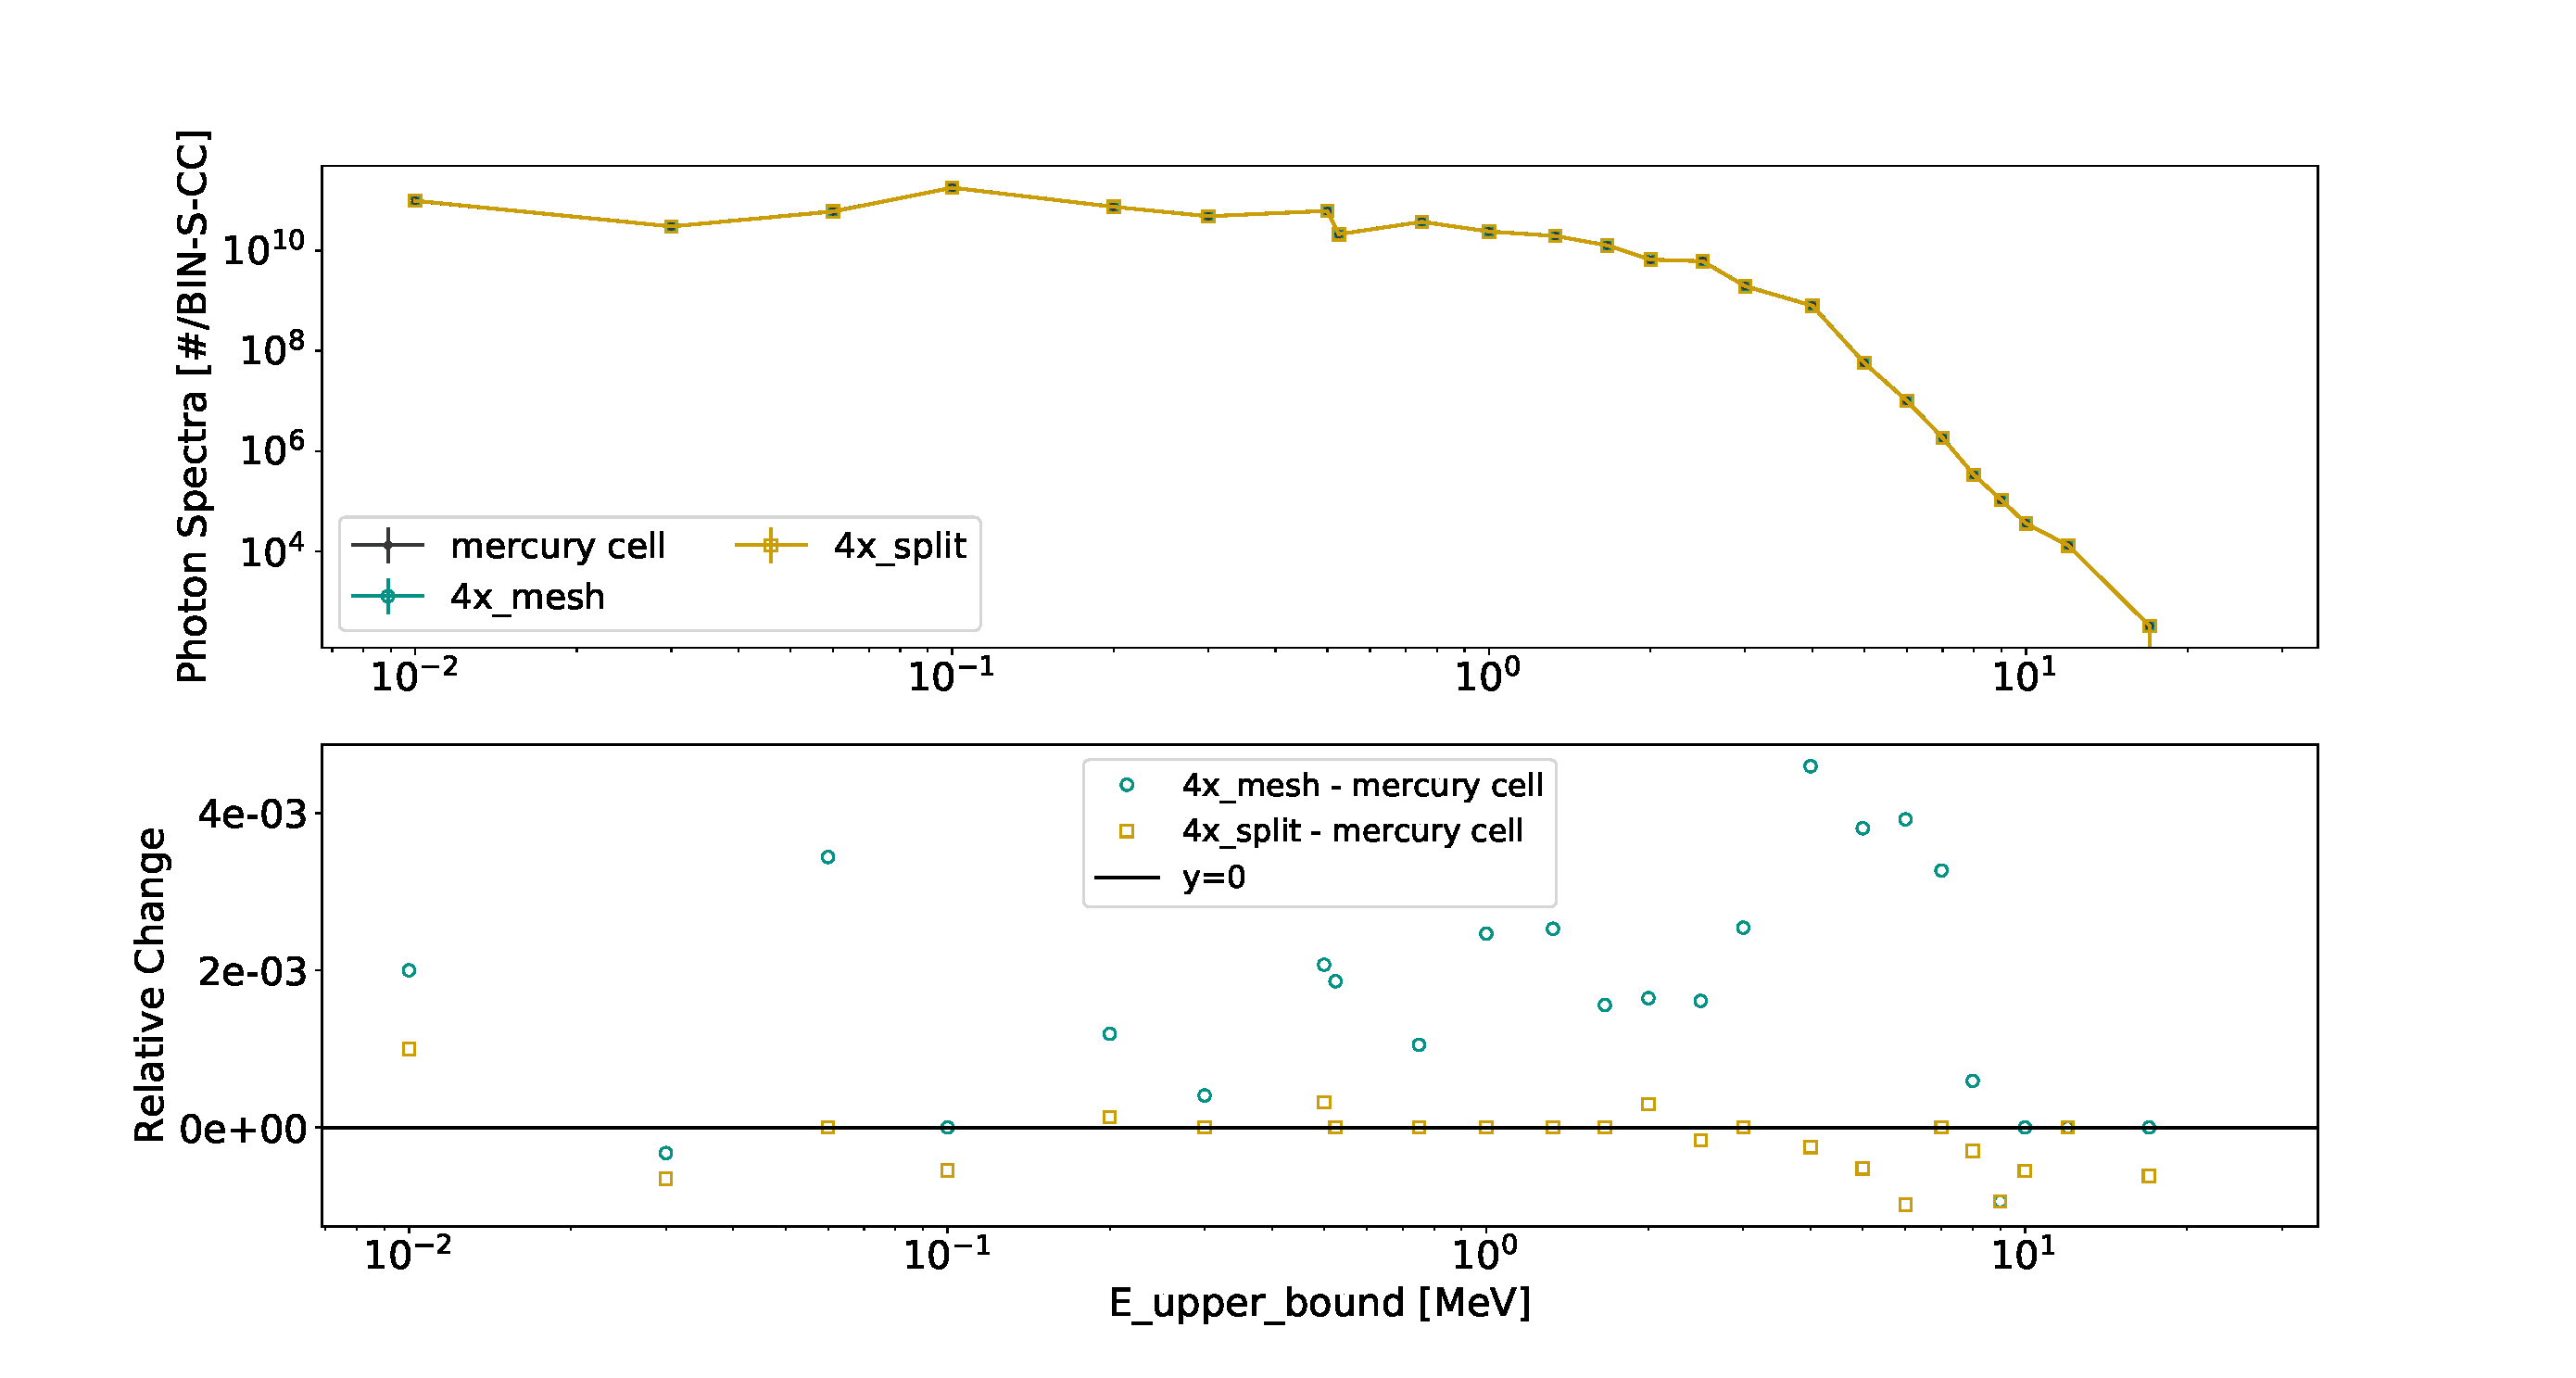
\includegraphics[scale=0.42,trim={2cm 0.5cm 3cm 2cm},clip]{../figs/toy_p1/spec_VPI_4x.pdf}
 \caption{Photon Spectrum in mercury cell, 4x4x4 mesh, and geometry split}
 \label{fig:1spec_cell_4x}
\end{figure}
Figure \ref{fig:1spec_8v} shows the results per voxel for a 2x2x2 mesh.
\begin{figure}
	\centering
	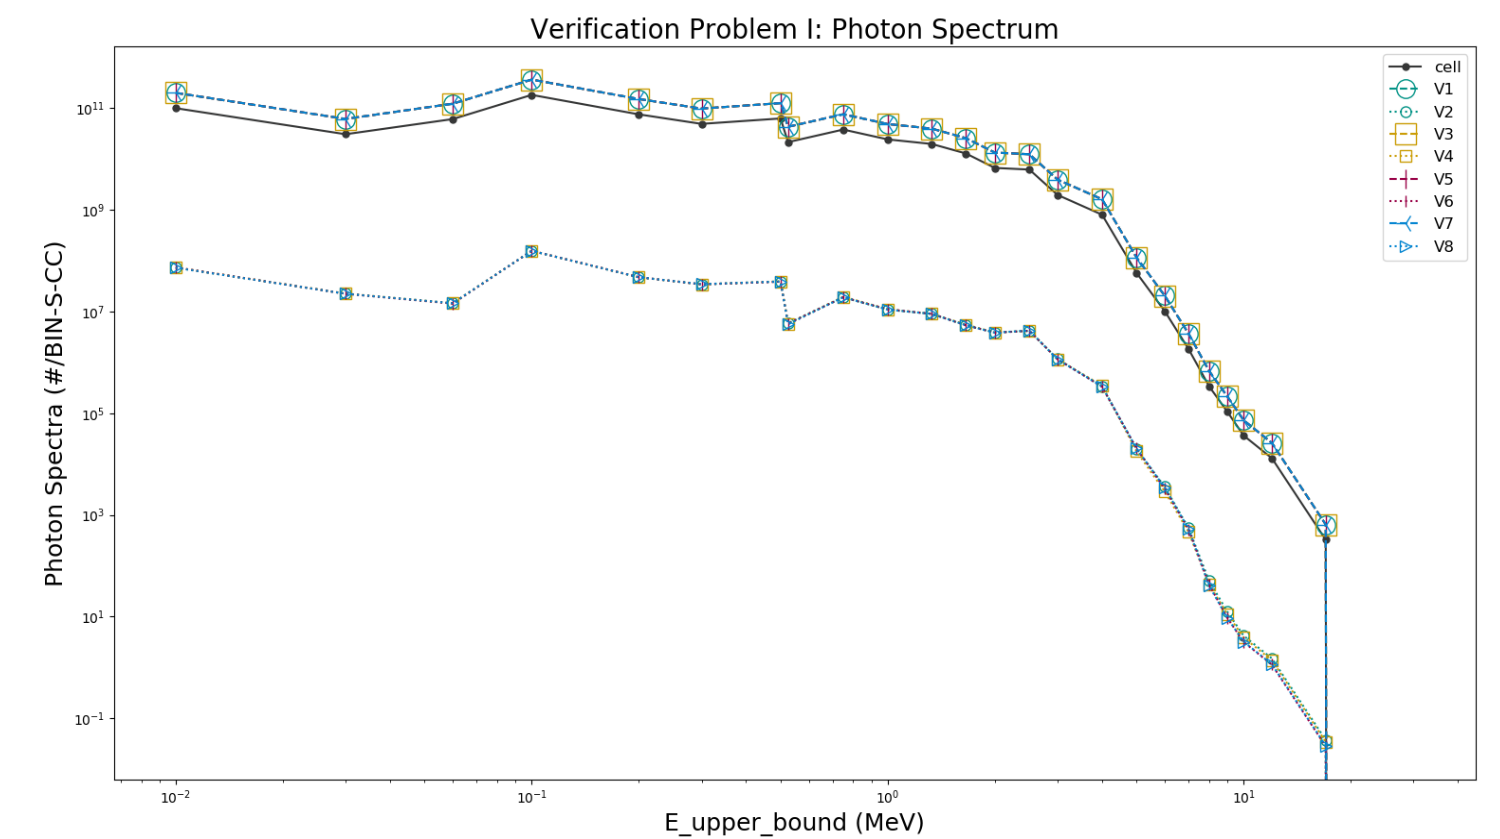
\includegraphics[scale=0.4, trim={1cm 0cm 0.5cm 1.25cm},clip]{../figs/toy_p1/spec_VPI_8.png}
	\caption{No sure}
	\label{fig:1spec_8v}
\end{figure}
\\
The biological dose was then calculated using the photon emission density.
Figures \ref{fig:1dose}
%
\begin{figure}
	\begin{subfigure}[t]{0.5\textwidth}
		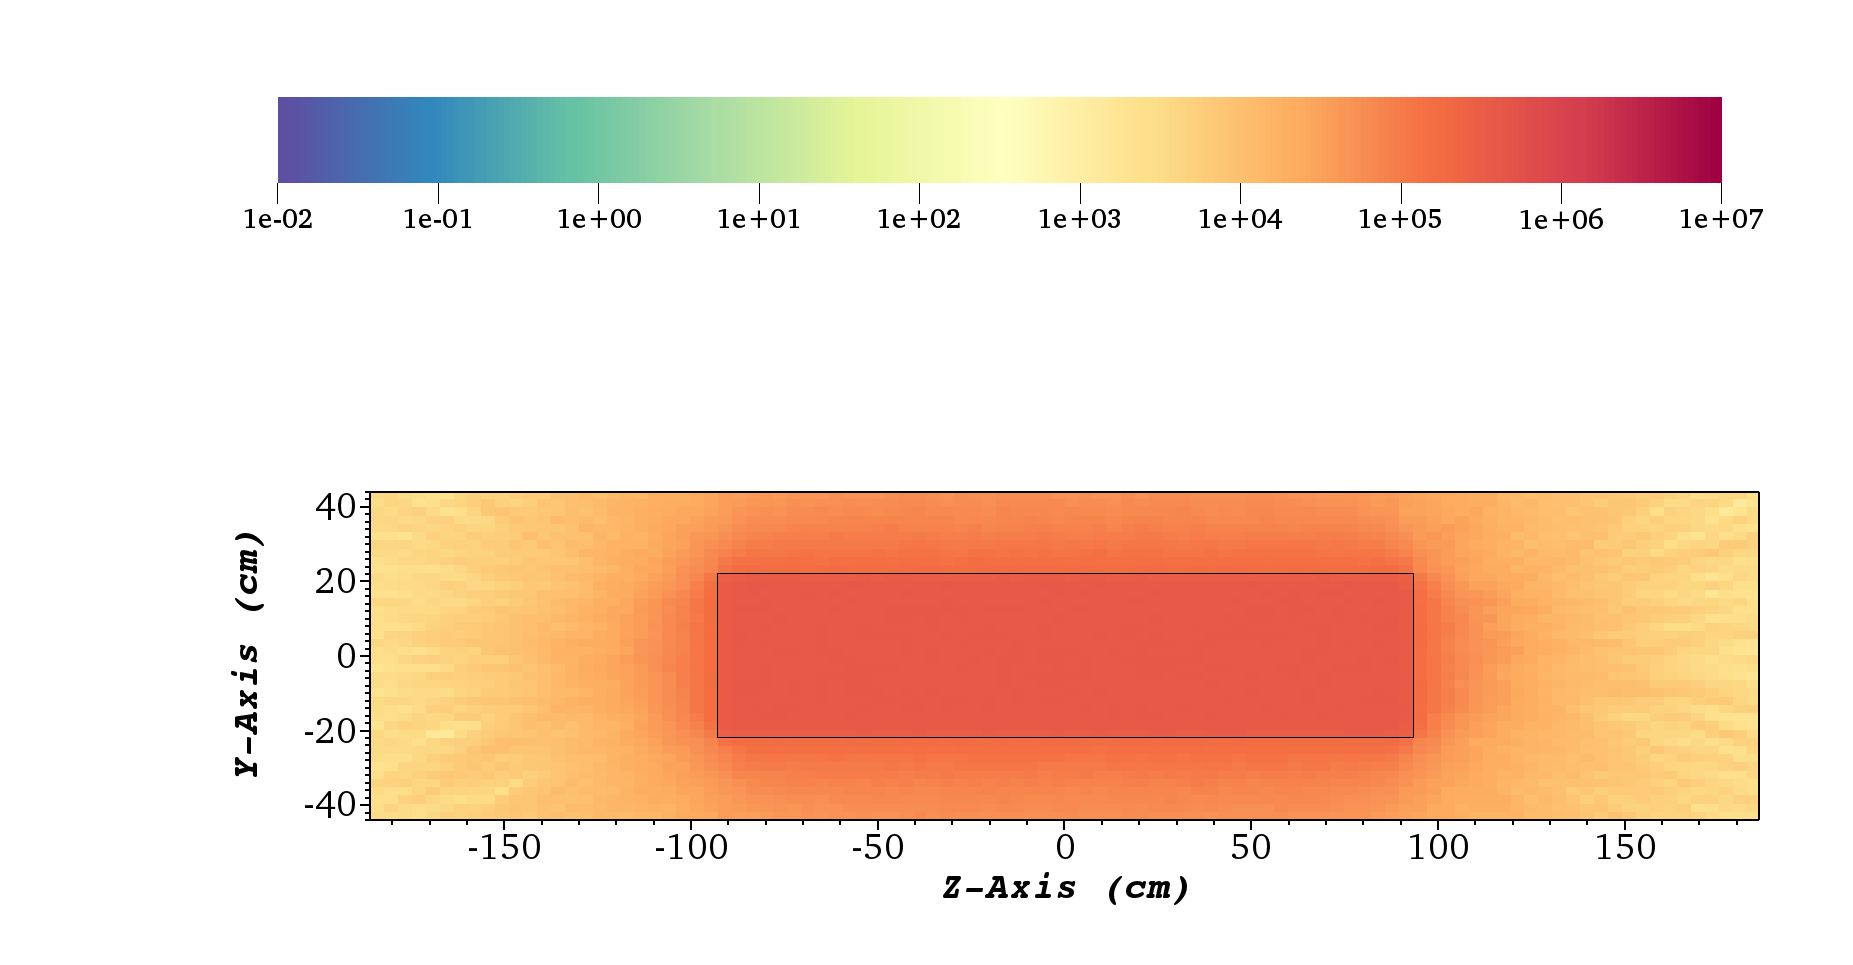
\includegraphics[width=\linewidth, trim={5cm 1cm 2cm 16cm},clip]{../figs/toy_p1/dose_VPI_original.png}
		\caption{full geometry}
		\label{fig:1dose_orig}
	\end{subfigure}\hfill
	\begin{subfigure}[t]{0.5\textwidth}
		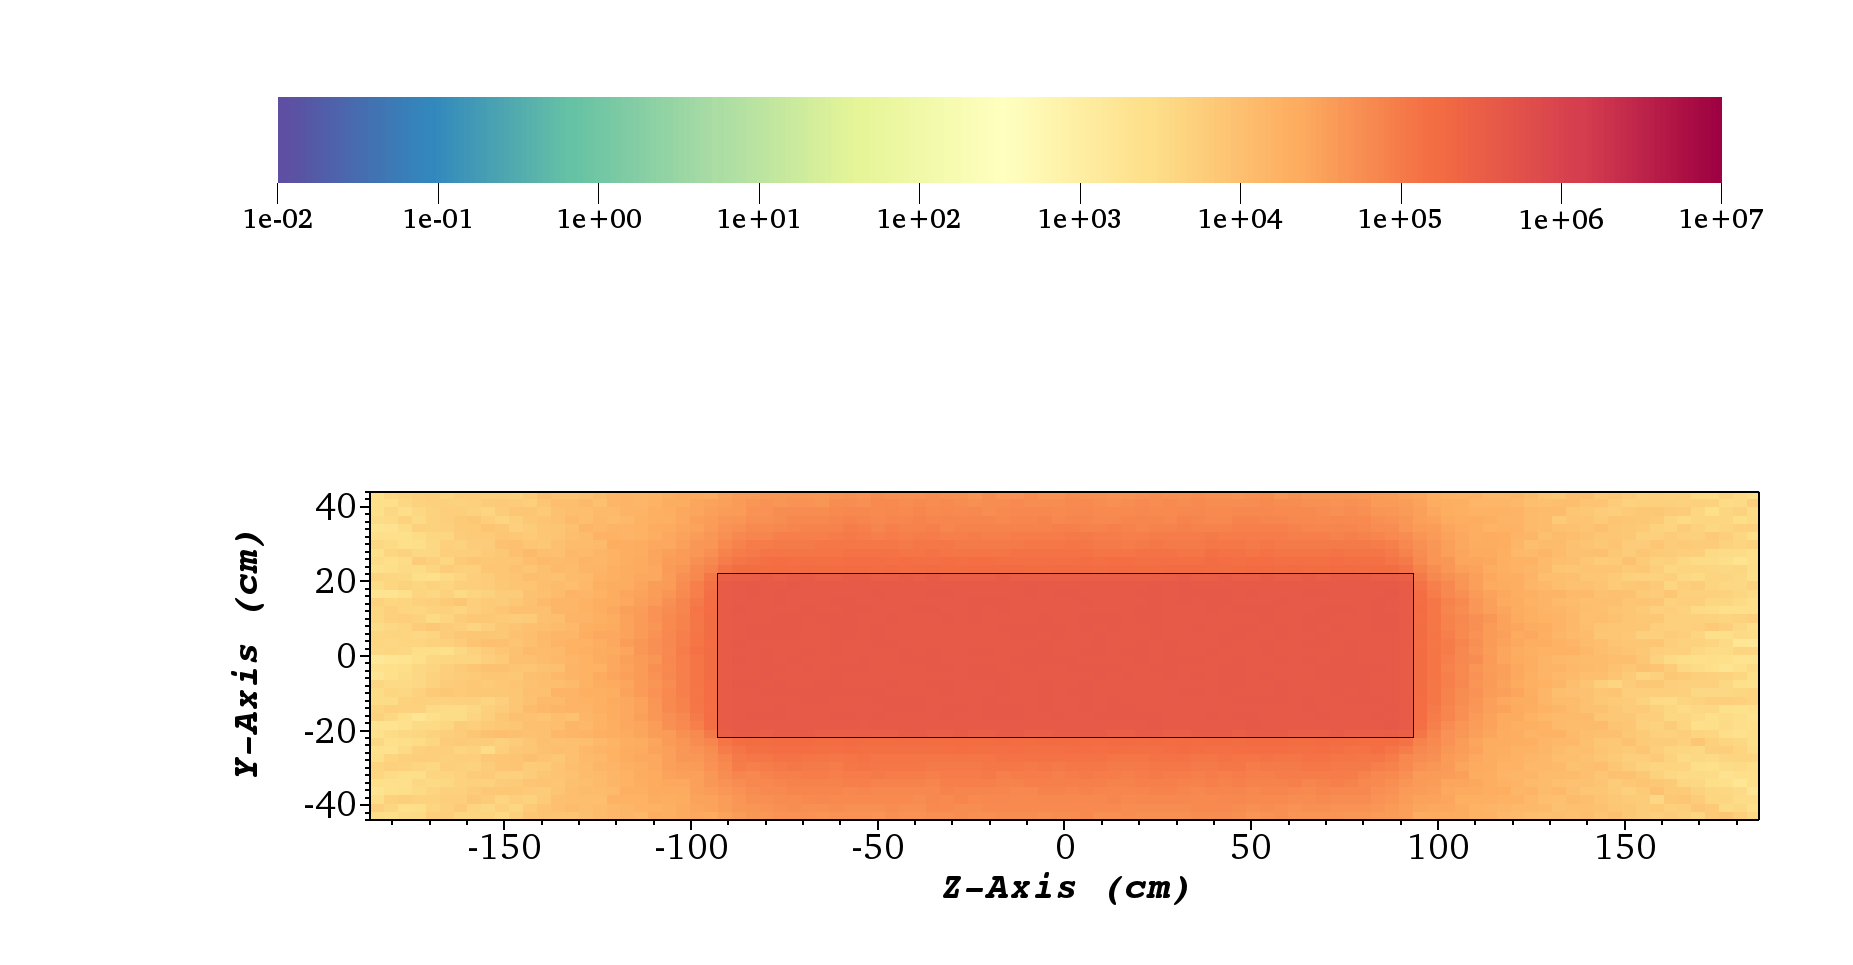
\includegraphics[width=\linewidth, trim={5cm 1cm 2cm 16cm},clip]{../figs/toy_p1/dose_VPI_1x_mesh.png}
		\caption{1x1x1 mesh}
		\label{fig:1dose_1x_mesh}
	\end{subfigure}

	\begin{subfigure}[t]{0.5\textwidth}
		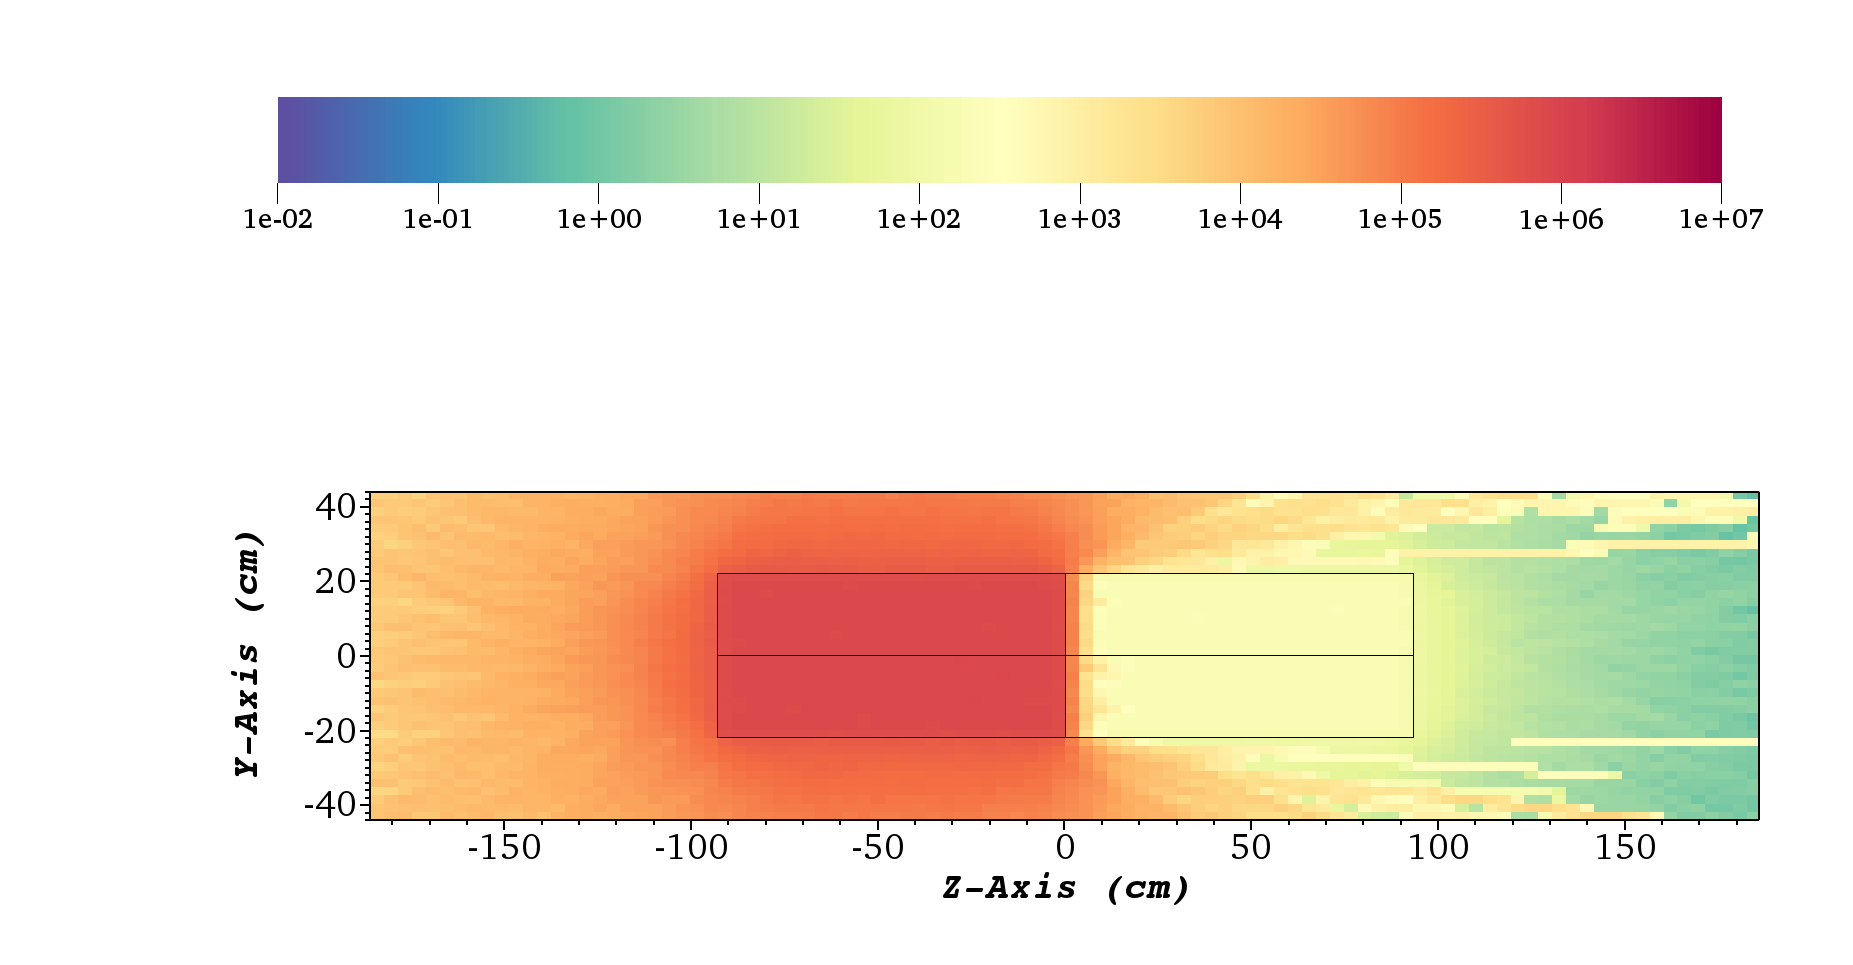
\includegraphics[width=\linewidth, trim={5cm 1cm 2cm 16cm},clip]{../figs/toy_p1/dose_VPI_2x_split.png}
		\caption{2x2x2 divided}
		\label{fig:1dose_2x_split}
	\end{subfigure}\hfill
	\begin{subfigure}[t]{0.5\textwidth}
		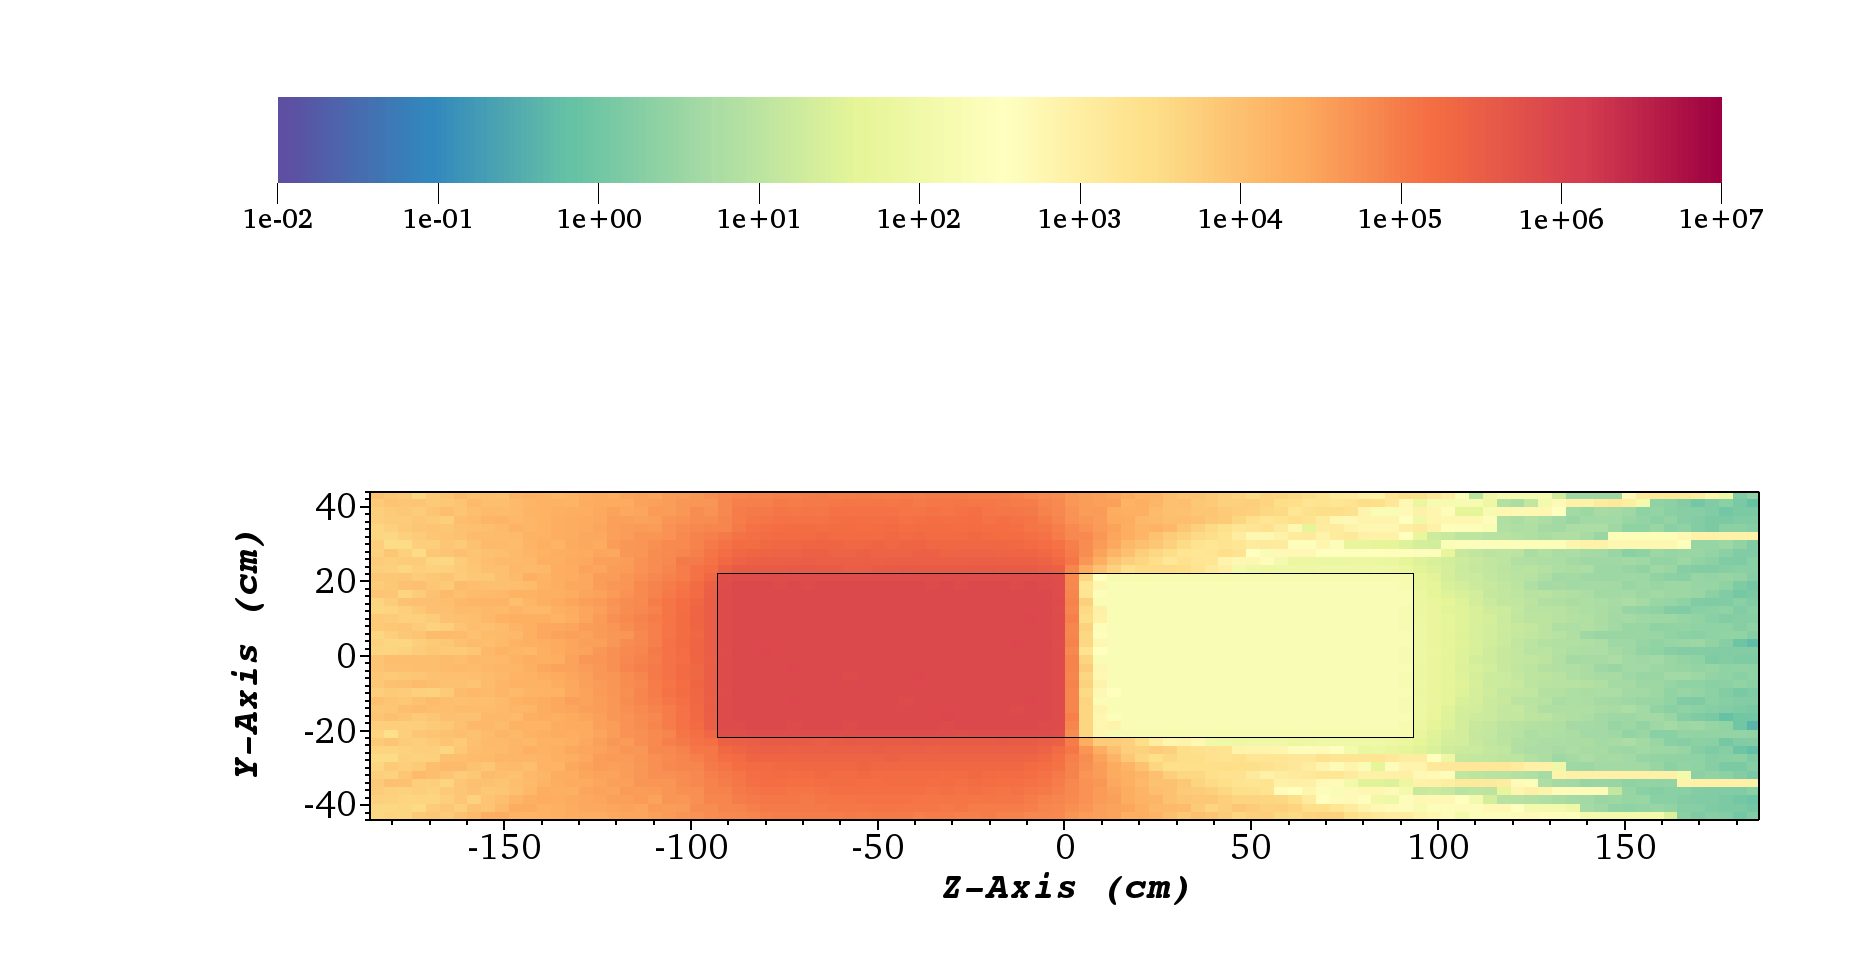
\includegraphics[width=\linewidth, trim={5cm 1cm 2cm 16cm},clip]{../figs/toy_p1/dose_VPI_2x_mesh.png}
		\caption{2x2x2 mesh}
		\label{fig:1dose_2x_mesh}
	\end{subfigure}

	\begin{subfigure}[t]{0.5\textwidth}
		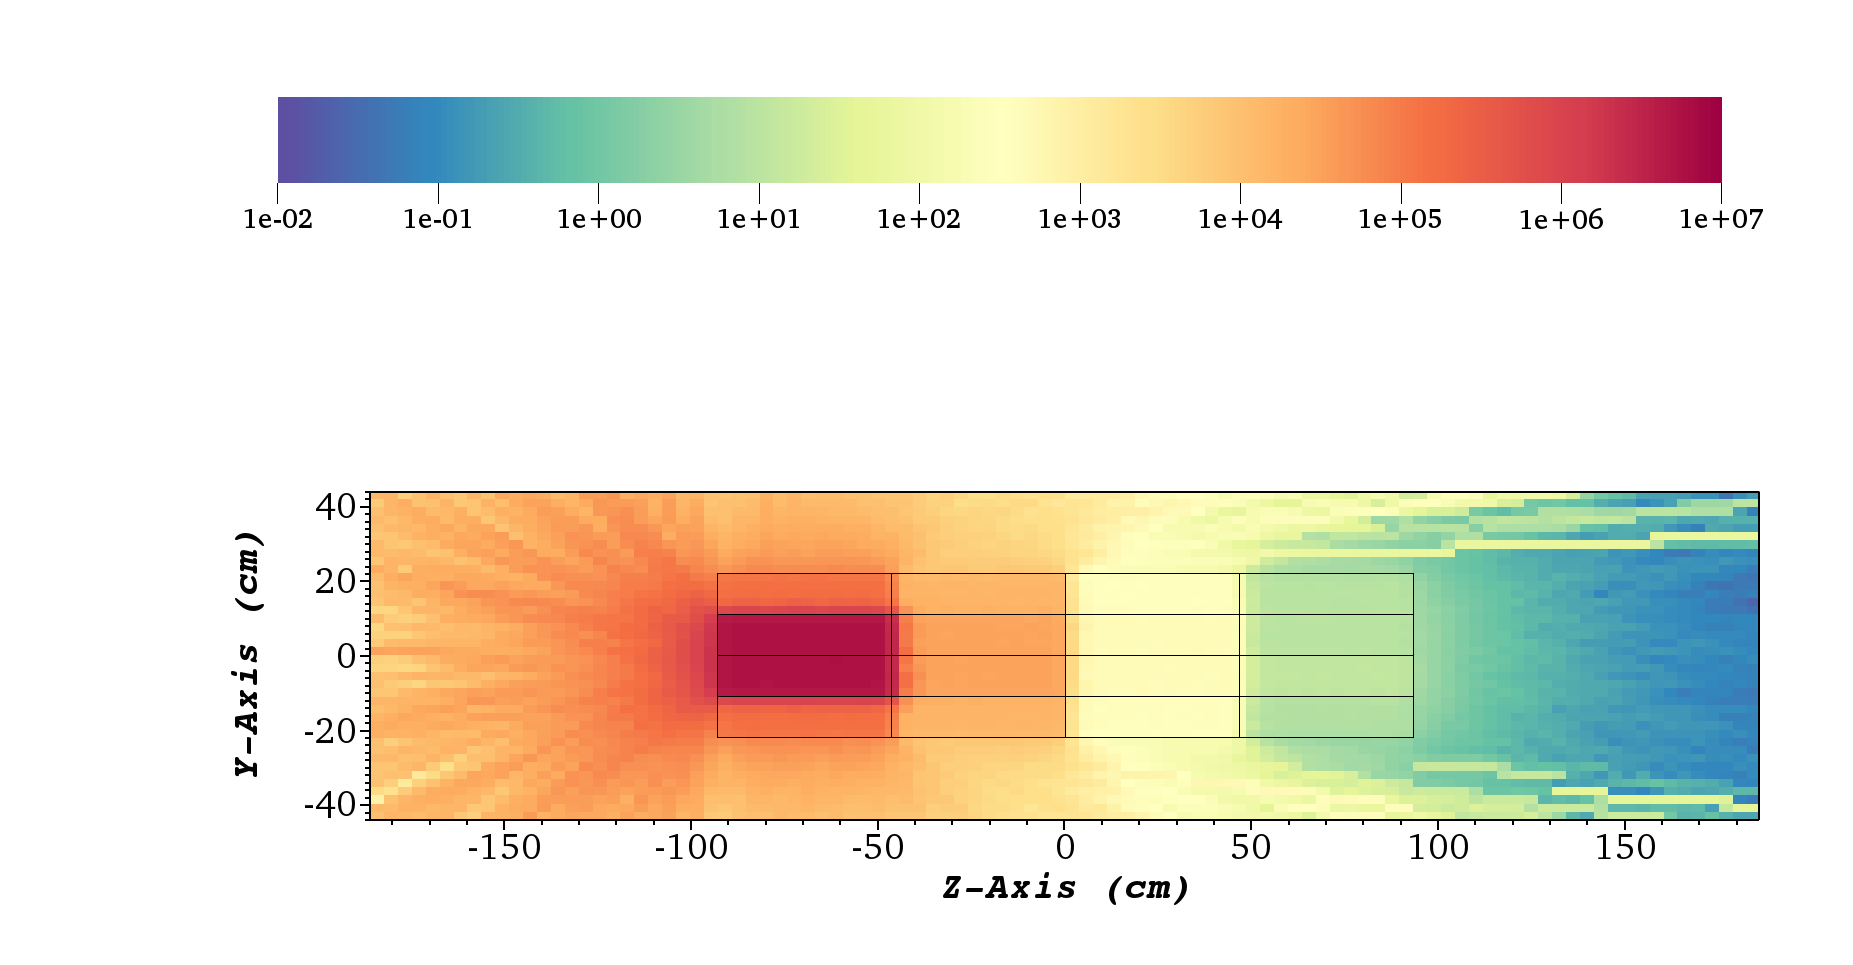
\includegraphics[width=\linewidth, trim={5cm 1cm 2cm 16cm},clip]{../figs/toy_p1/dose_VPI_4x_split.png}
		\caption{4x4x4 divided}
		\label{fig:1dose_4x_split}
	\end{subfigure}\hfill
	\begin{subfigure}[t]{0.5\textwidth}
		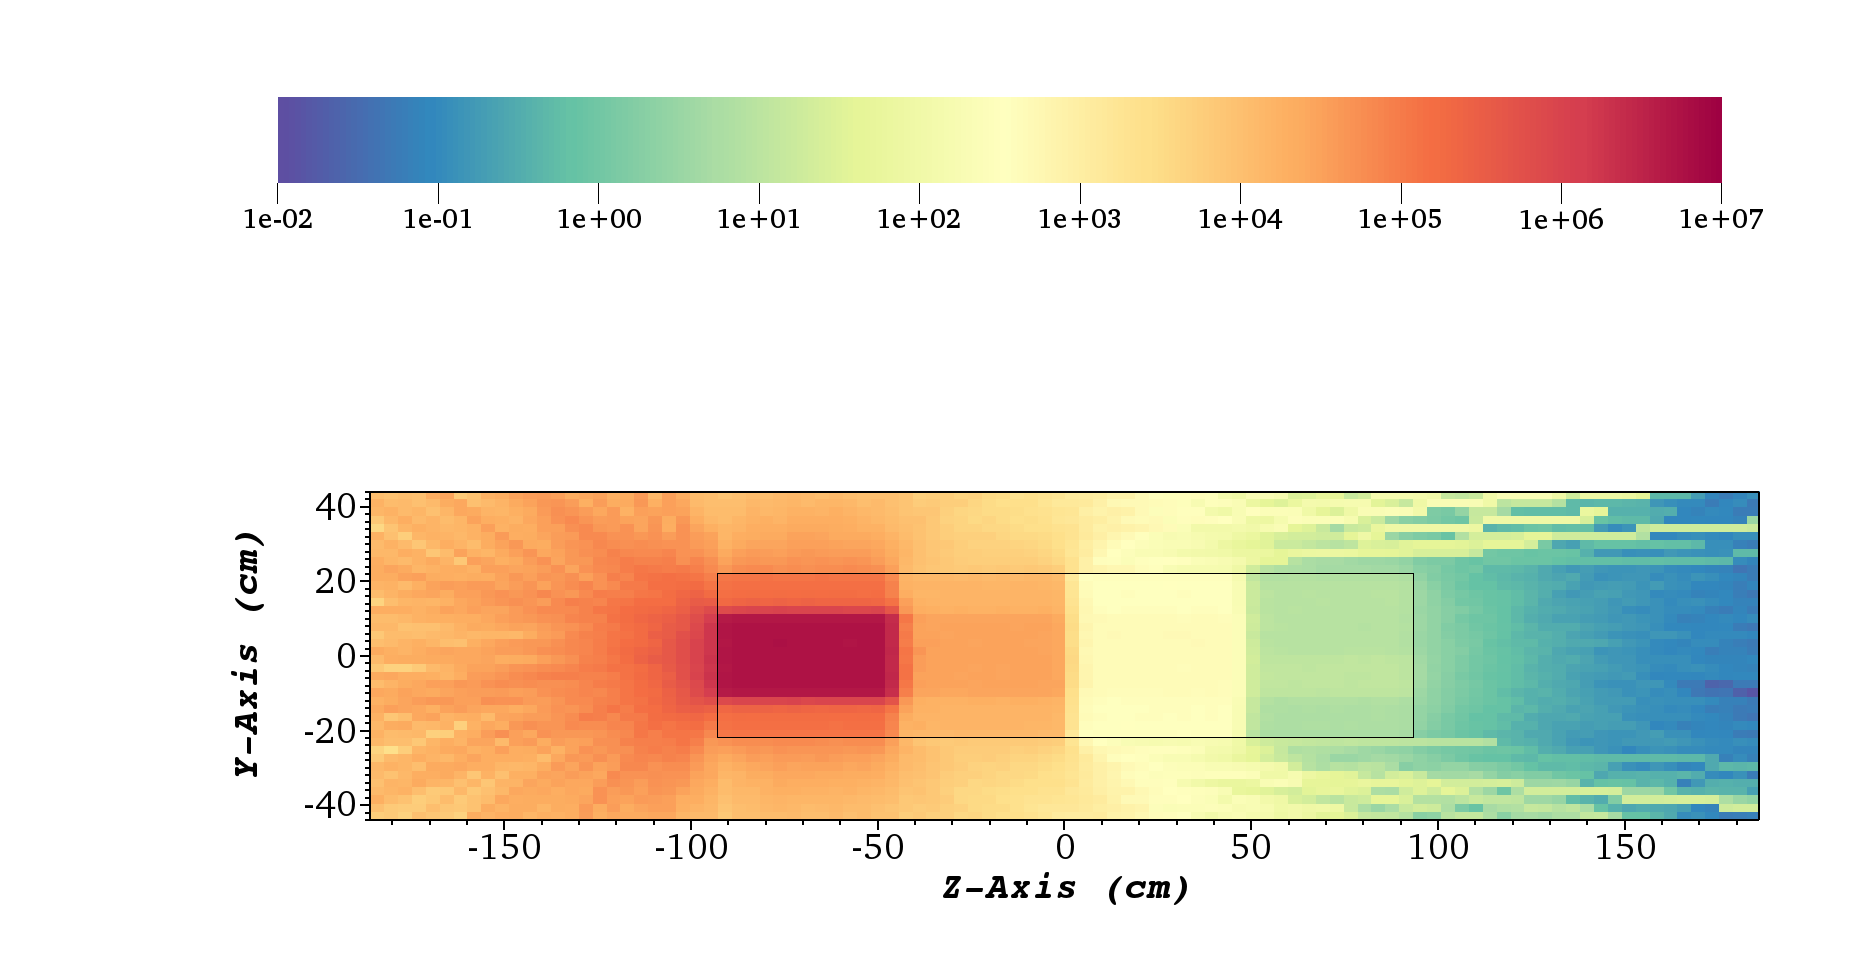
\includegraphics[width=\linewidth, trim={5cm 1cm 2cm 16cm},clip]{../figs/toy_p1/dose_VPI_4x_mesh.png}
		\caption{4x4x4 mesh}
		\label{fig:1dose_4x_mesh}
	\end{subfigure}

	\begin{subfigure}[t]{1.0\textwidth}
		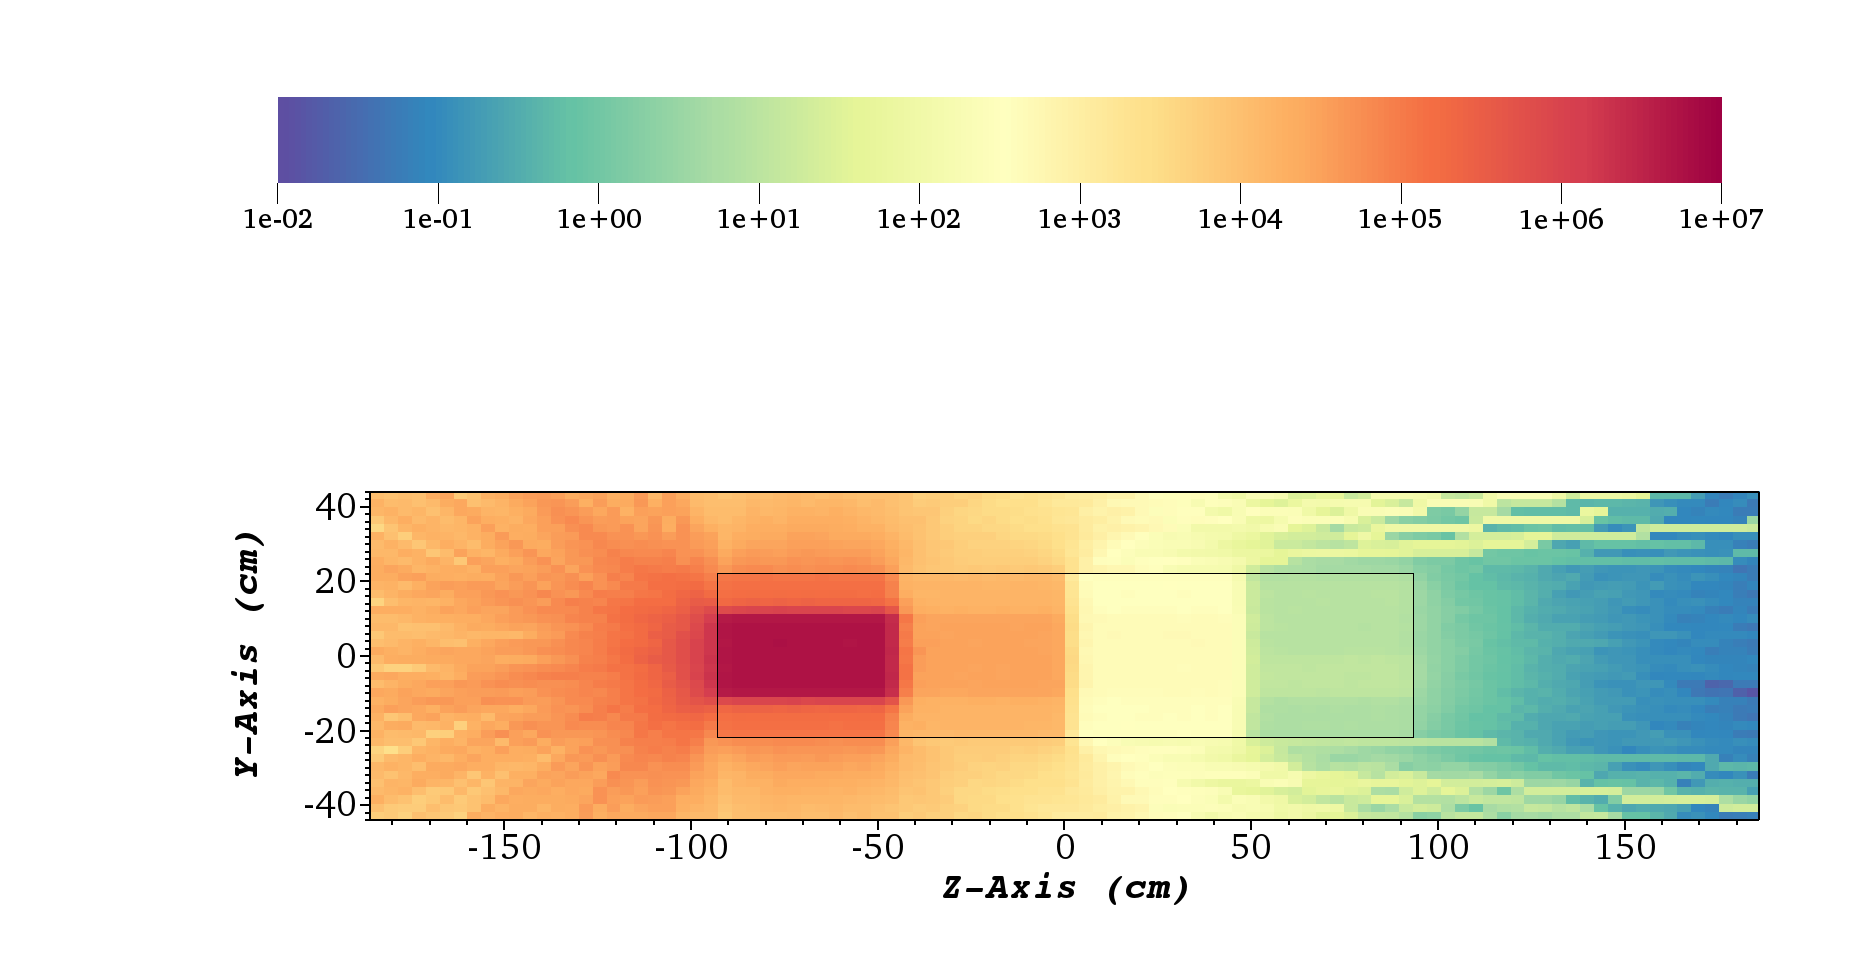
\includegraphics[width=\linewidth, trim={5cm 25cm 2cm 2cm},clip]{../figs/toy_p1/dose_VPI_4x_mesh.png}
		\label{fig:1legend}
	\end{subfigure}
	\caption{Biological dose rate on the mercury cell with mesh and divided geometry}
	\label{fig:1dose}
\end{figure}
\\
A z score was done to compare between the results from the mesh workflow and the results
obtained with the cell based workflow. The results can be seen in Figure \ref{fig:}

\begin{figure}
	\begin{subfigure}[h]{0.5\textwidth}
		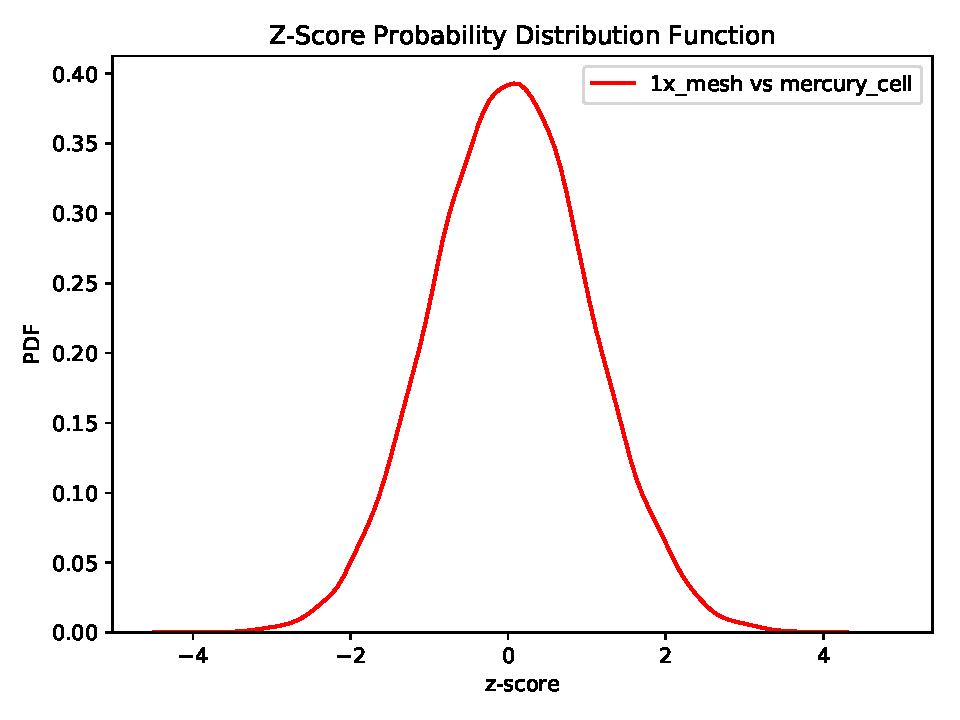
\includegraphics[width=\linewidth, trim={0cm 0cm 0cm 0.9cm},clip]{../figs/toy_p1/PDF_zscore_VPI_1x_orig.pdf}
		%\caption{PDF: 1x1x1x mesh to full geometry}
		\label{fig:1pdf_1x_orig}
	\end{subfigure}\hfill
	\begin{subfigure}[h]{0.5\textwidth}
		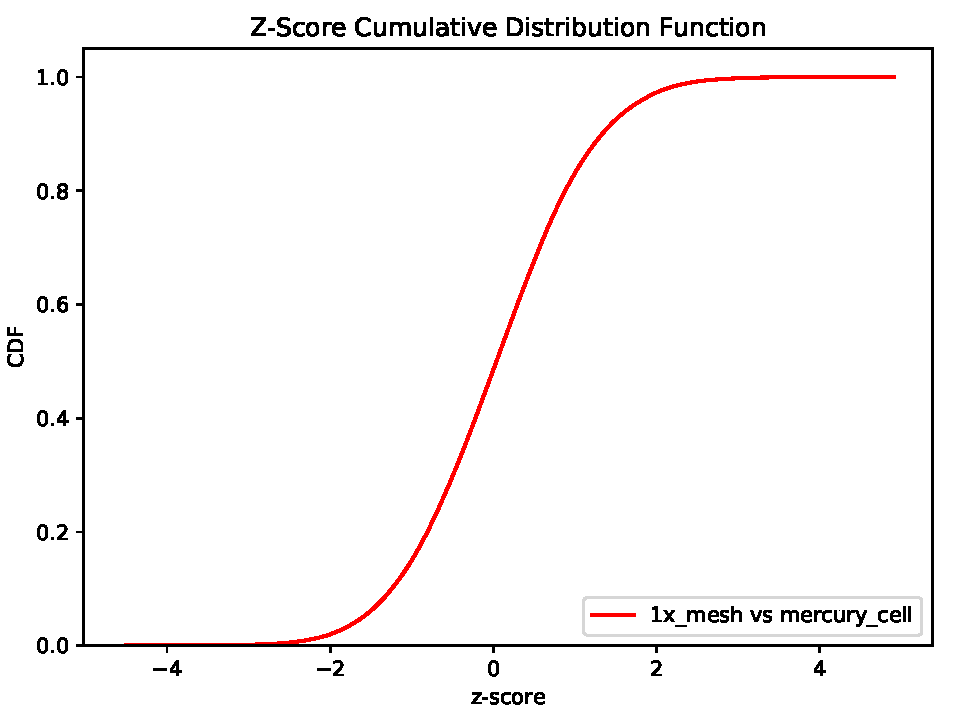
\includegraphics[width=\linewidth, trim={0cm 0cm 0cm 0.8cm},clip]{../figs/toy_p1/CDF_zscore_VPI_1x_orig.pdf}
		% \caption{CDF: 1x1x1 mesh to full geometry}
		\label{fig:1cdf_1x_orig}
	\end{subfigure}

	\begin{subfigure}[h]{0.5\textwidth}
		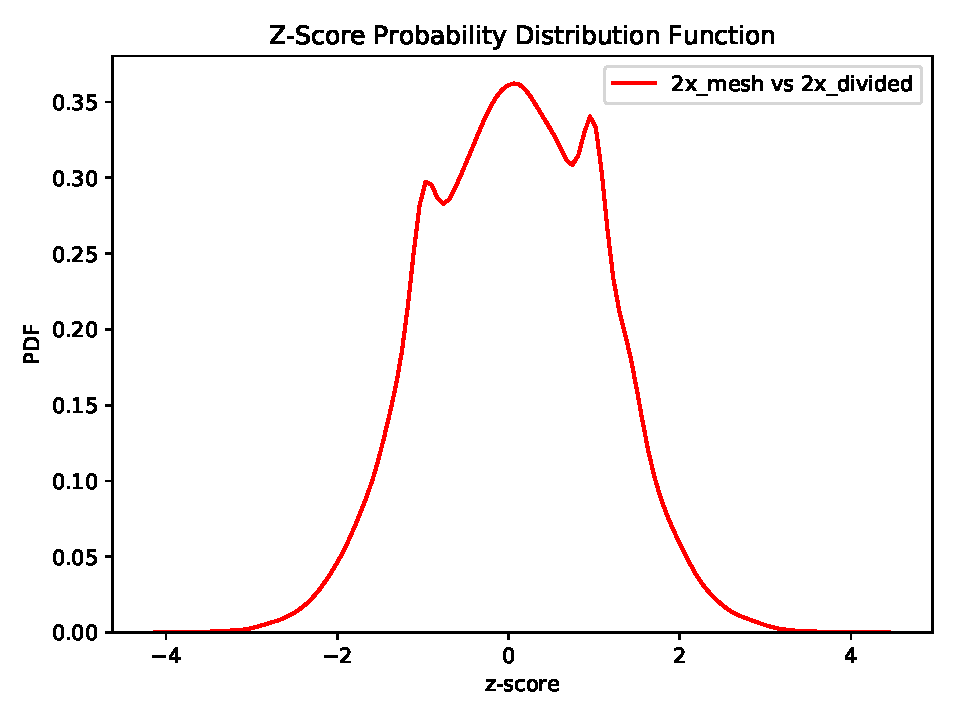
\includegraphics[width=\linewidth, trim={0cm 0cm 0cm 0.9cm},clip]{../figs/toy_p1/PDF_zscore_VPI_2xm_2xs.pdf}
		% \caption{2x2x2 divided}
		\label{fig:1dose_2x_split}
	\end{subfigure}\hfill
	\begin{subfigure}[h]{0.5\textwidth}
		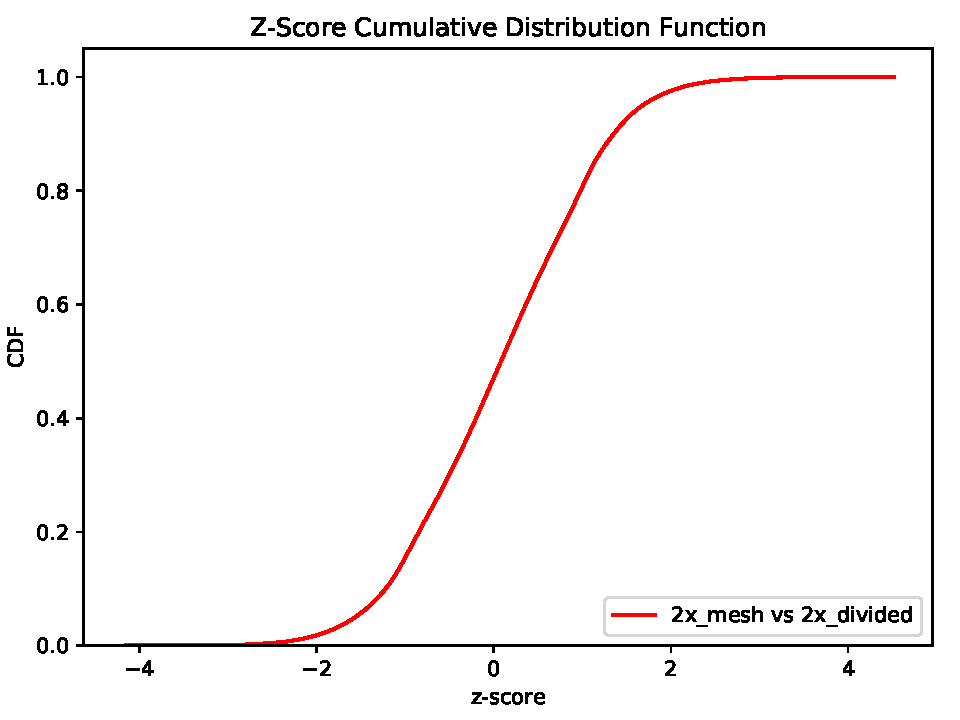
\includegraphics[width=\linewidth, trim={0cm 0cm 0cm 0.8cm},clip]{../figs/toy_p1/CDF_zscore_VPI_2xm_2xs.pdf}
		% \caption{2x2x2 mesh}
		\label{fig:1dose_2x_mesh}
	\end{subfigure}

	\begin{subfigure}[t]{0.5\textwidth}
		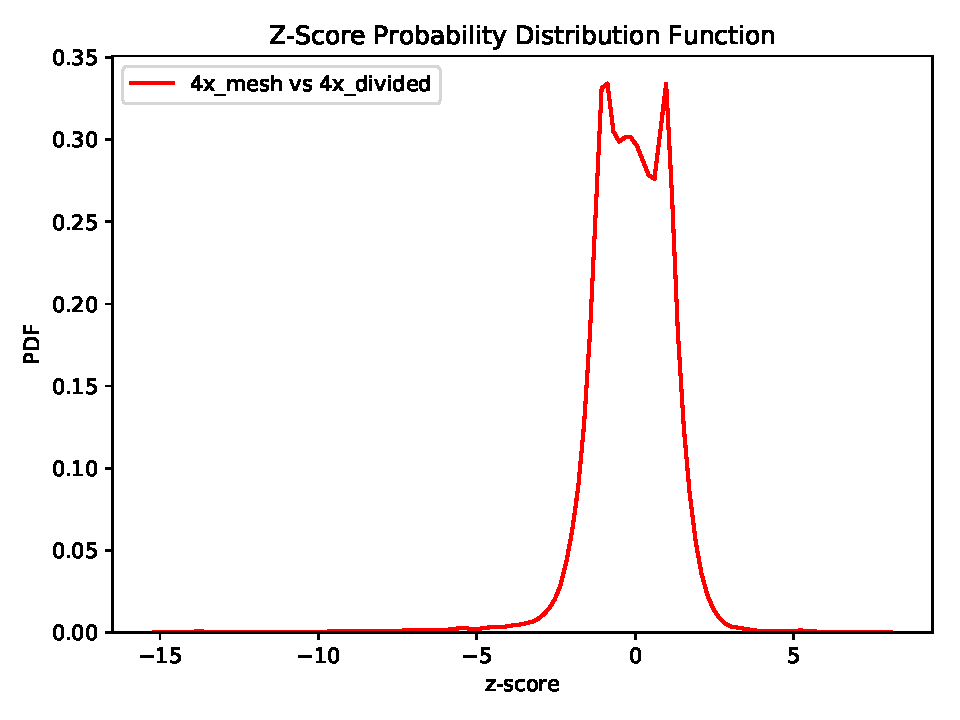
\includegraphics[width=\linewidth, trim={0cm 0cm 0cm 0.9cm},clip]{../figs/toy_p1/PDF_zscore_VPI_4xm_4xs.pdf}
		% \caption{4x4x4 divided}
		\label{fig:1dose_4x_split}
	\end{subfigure}\hfill
	\begin{subfigure}[t]{0.5\textwidth}
		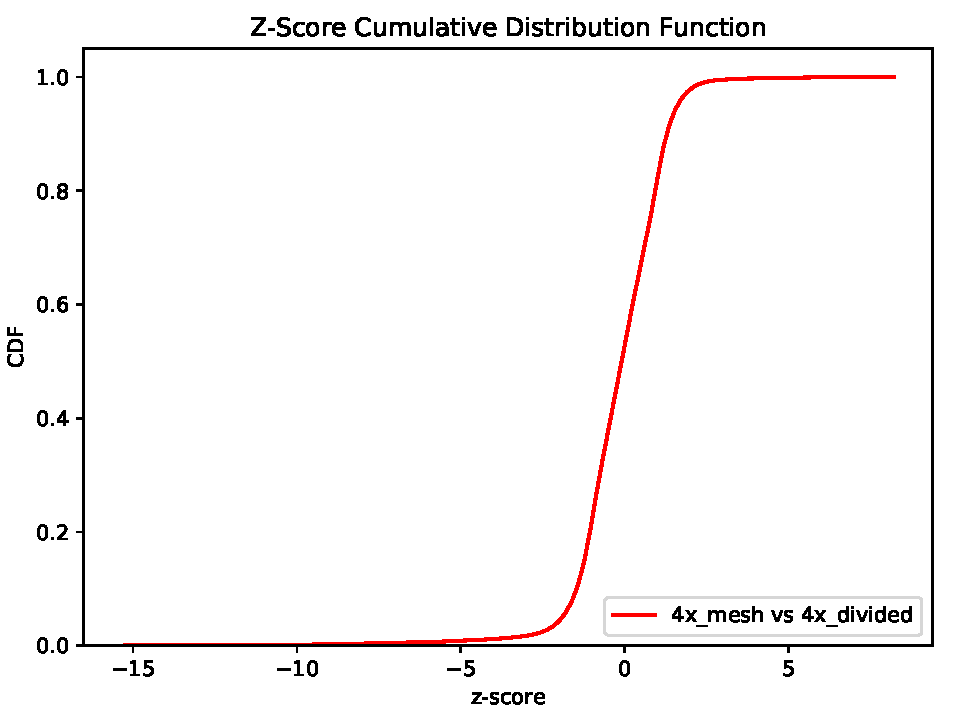
\includegraphics[width=\linewidth, trim={0cm 0cm 0cm 0.8cm},clip]{../figs/toy_p1/CDF_zscore_VPI_4xm_4xs.pdf}
		% \caption{4x4x4 mesh}
		\label{fig:1dose_4x_mesh}
	\end{subfigure}
	\caption{Z scores PDF and CDF comparing the results for the mesh to respective divided geometry }
	\label{fig:1dose}
\end{figure}

%%%%%%%%%%%%%%%%%%

\newpage

\subsubsection{Verification Problem II}
Similar analysis were done for the second verification problem. Figure
\ref{fig:2prod_cell_1x_2x_4x} show the results collected in the mercury and
steel cell as well as the results for the three meshes. The results for the
mercury and steel cell were added and the results of each voxel in mesh were
added to directly compare the total results.
%
\begin{figure}[h!]
 \centering
 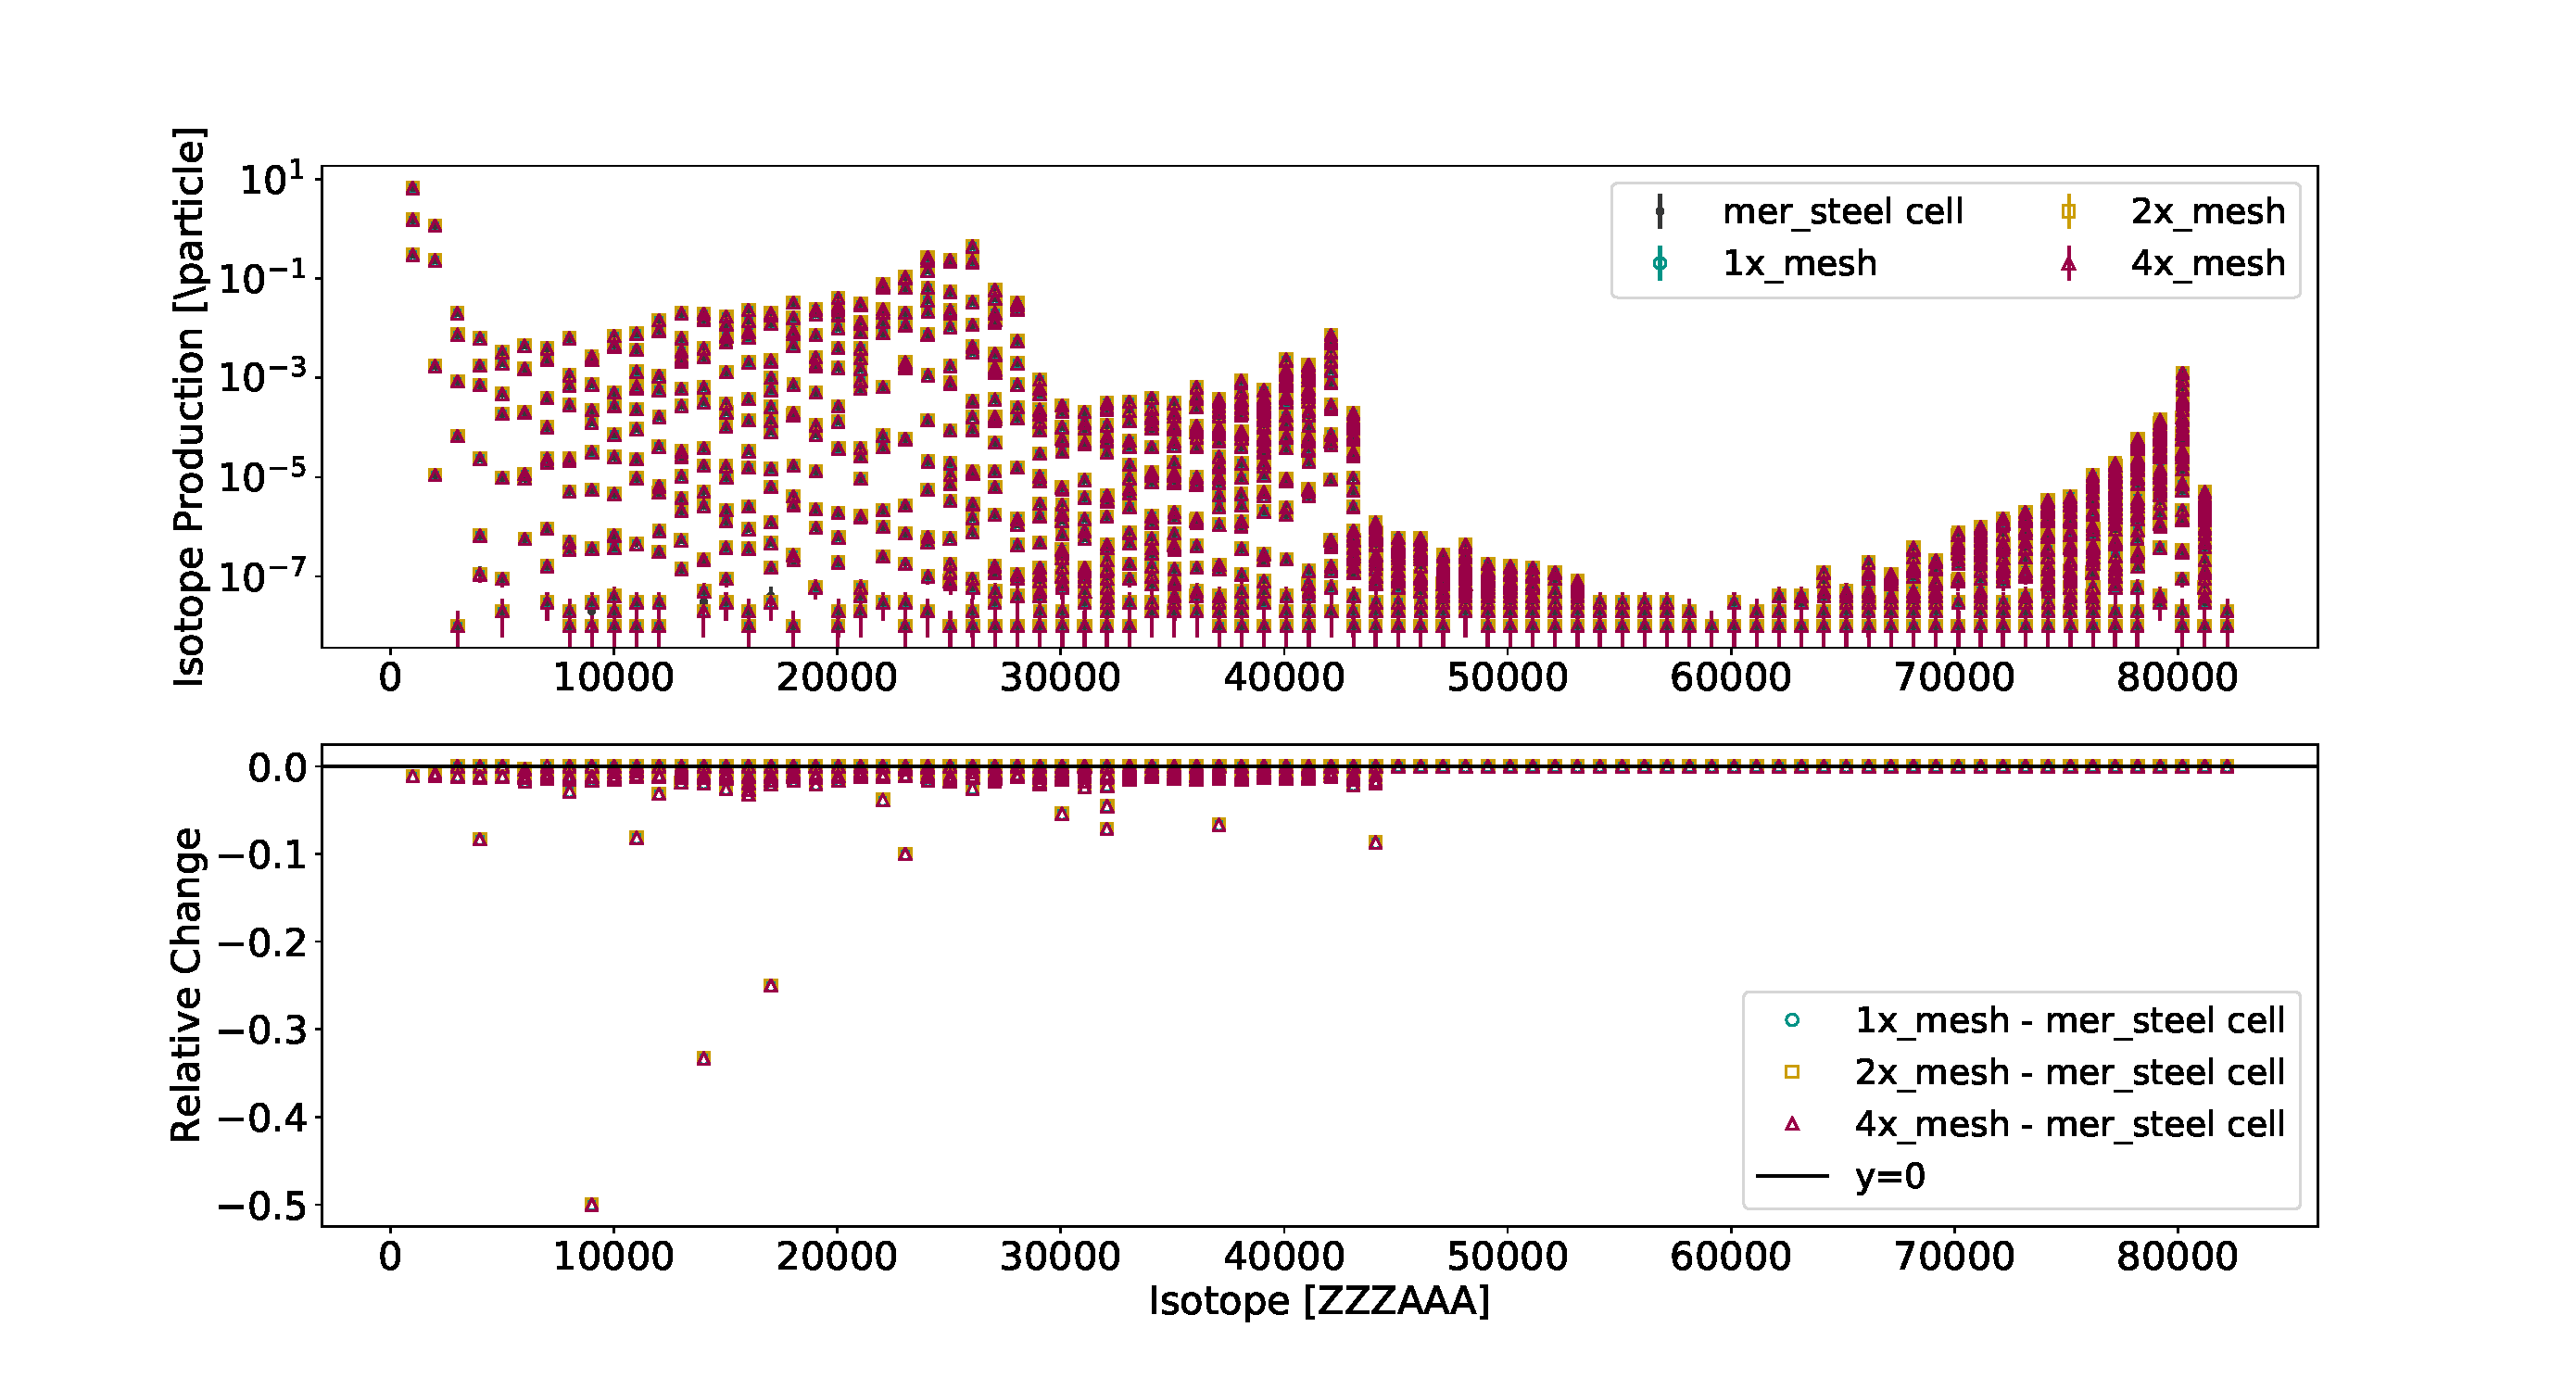
\includegraphics[scale=0.42,trim={2cm 1cm 3cm 2cm},clip]{../figs/toy_p2/prod_VPII_1x_2x_4x.pdf}
 \caption{Radionuclide production for mercury/steel cells and Cartesian meshes}
 \label{fig:2prod_cell_1x_2x_4x}
\end{figure}
%
\\
Figure \ref{fig:2prod_cell_2x} compares the results collected in the geometric
cell, the summed up results of the 2x2x2 mesh and the 2x2x2 divided geometry.
%
\begin{figure}[h!]
 \centering
 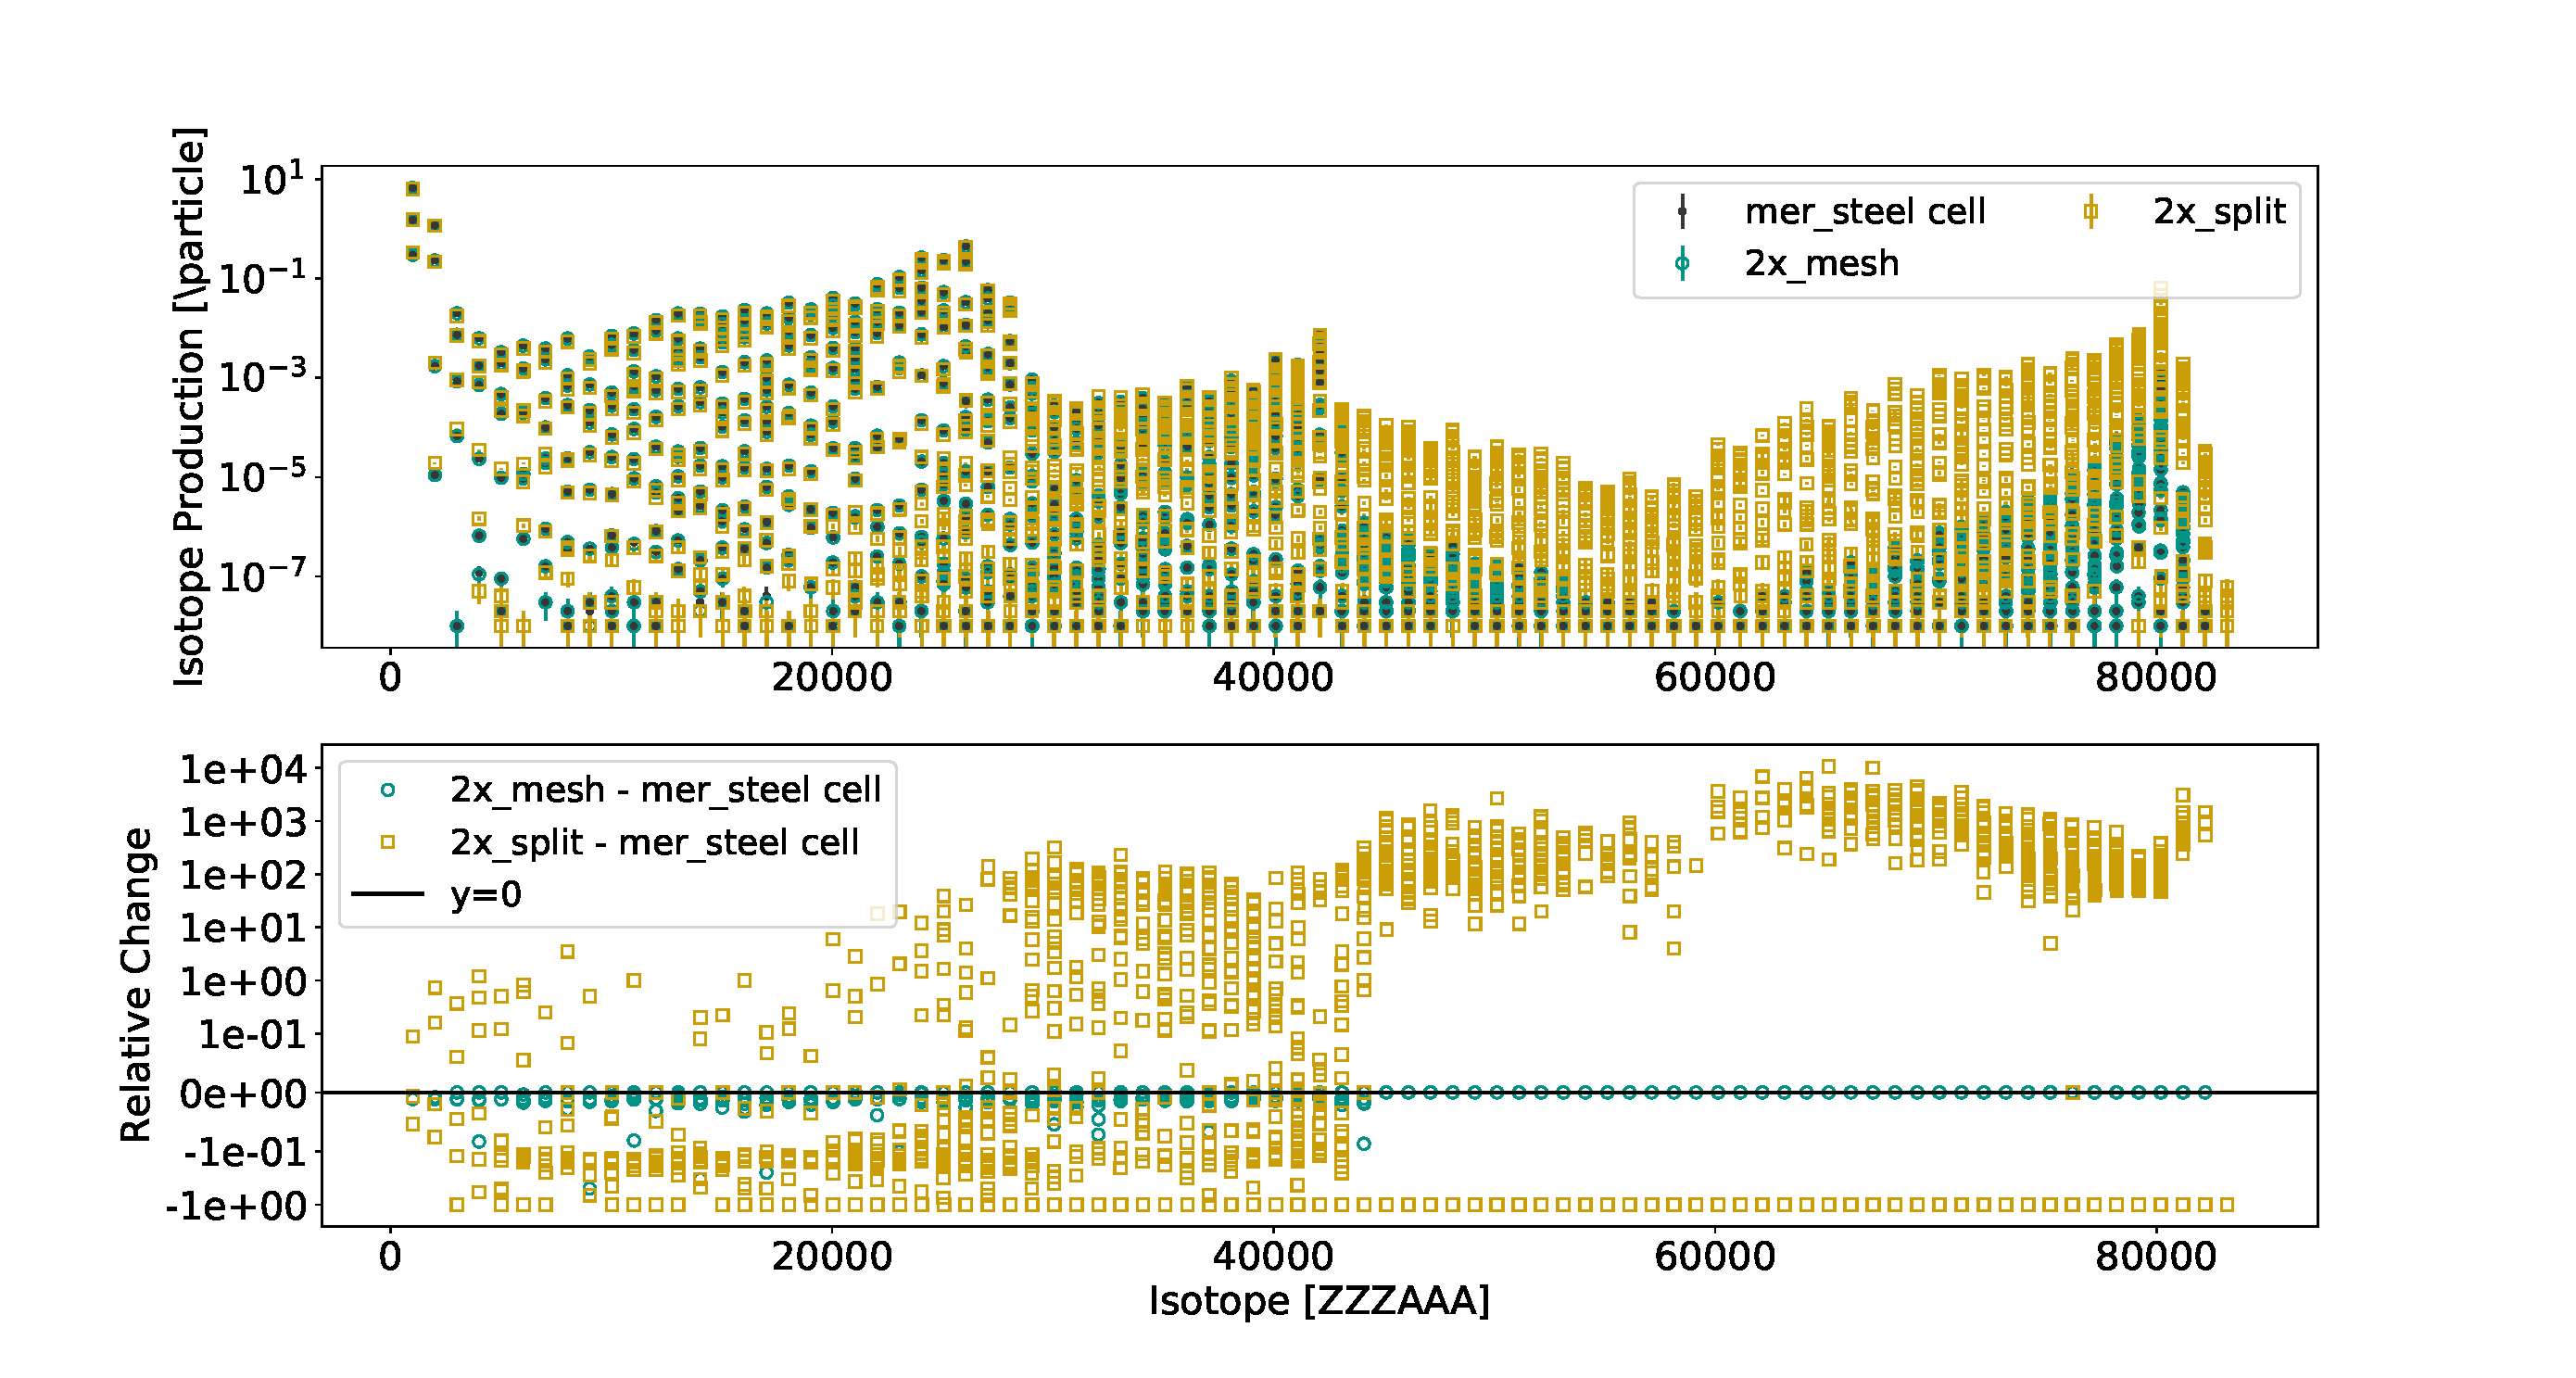
\includegraphics[scale=0.42,trim={2cm 1cm 3cm 2cm},clip]{../figs/toy_p2/prod_VPII_2x.pdf}
 \caption{Radionuclide production mercury/steel cells, 2x2x2 mesh, and 2x2x2 divided geometry}
 \label{fig:2prod_cell_2x}
\end{figure}
%
\\
A similar comparison was made for the 4x4x4 mesh and the 4x4x4 divided geometry
which can be seen in Figure \ref{fig:2prod_cell_4x}
%
\begin{figure}[h!]
 \centering
 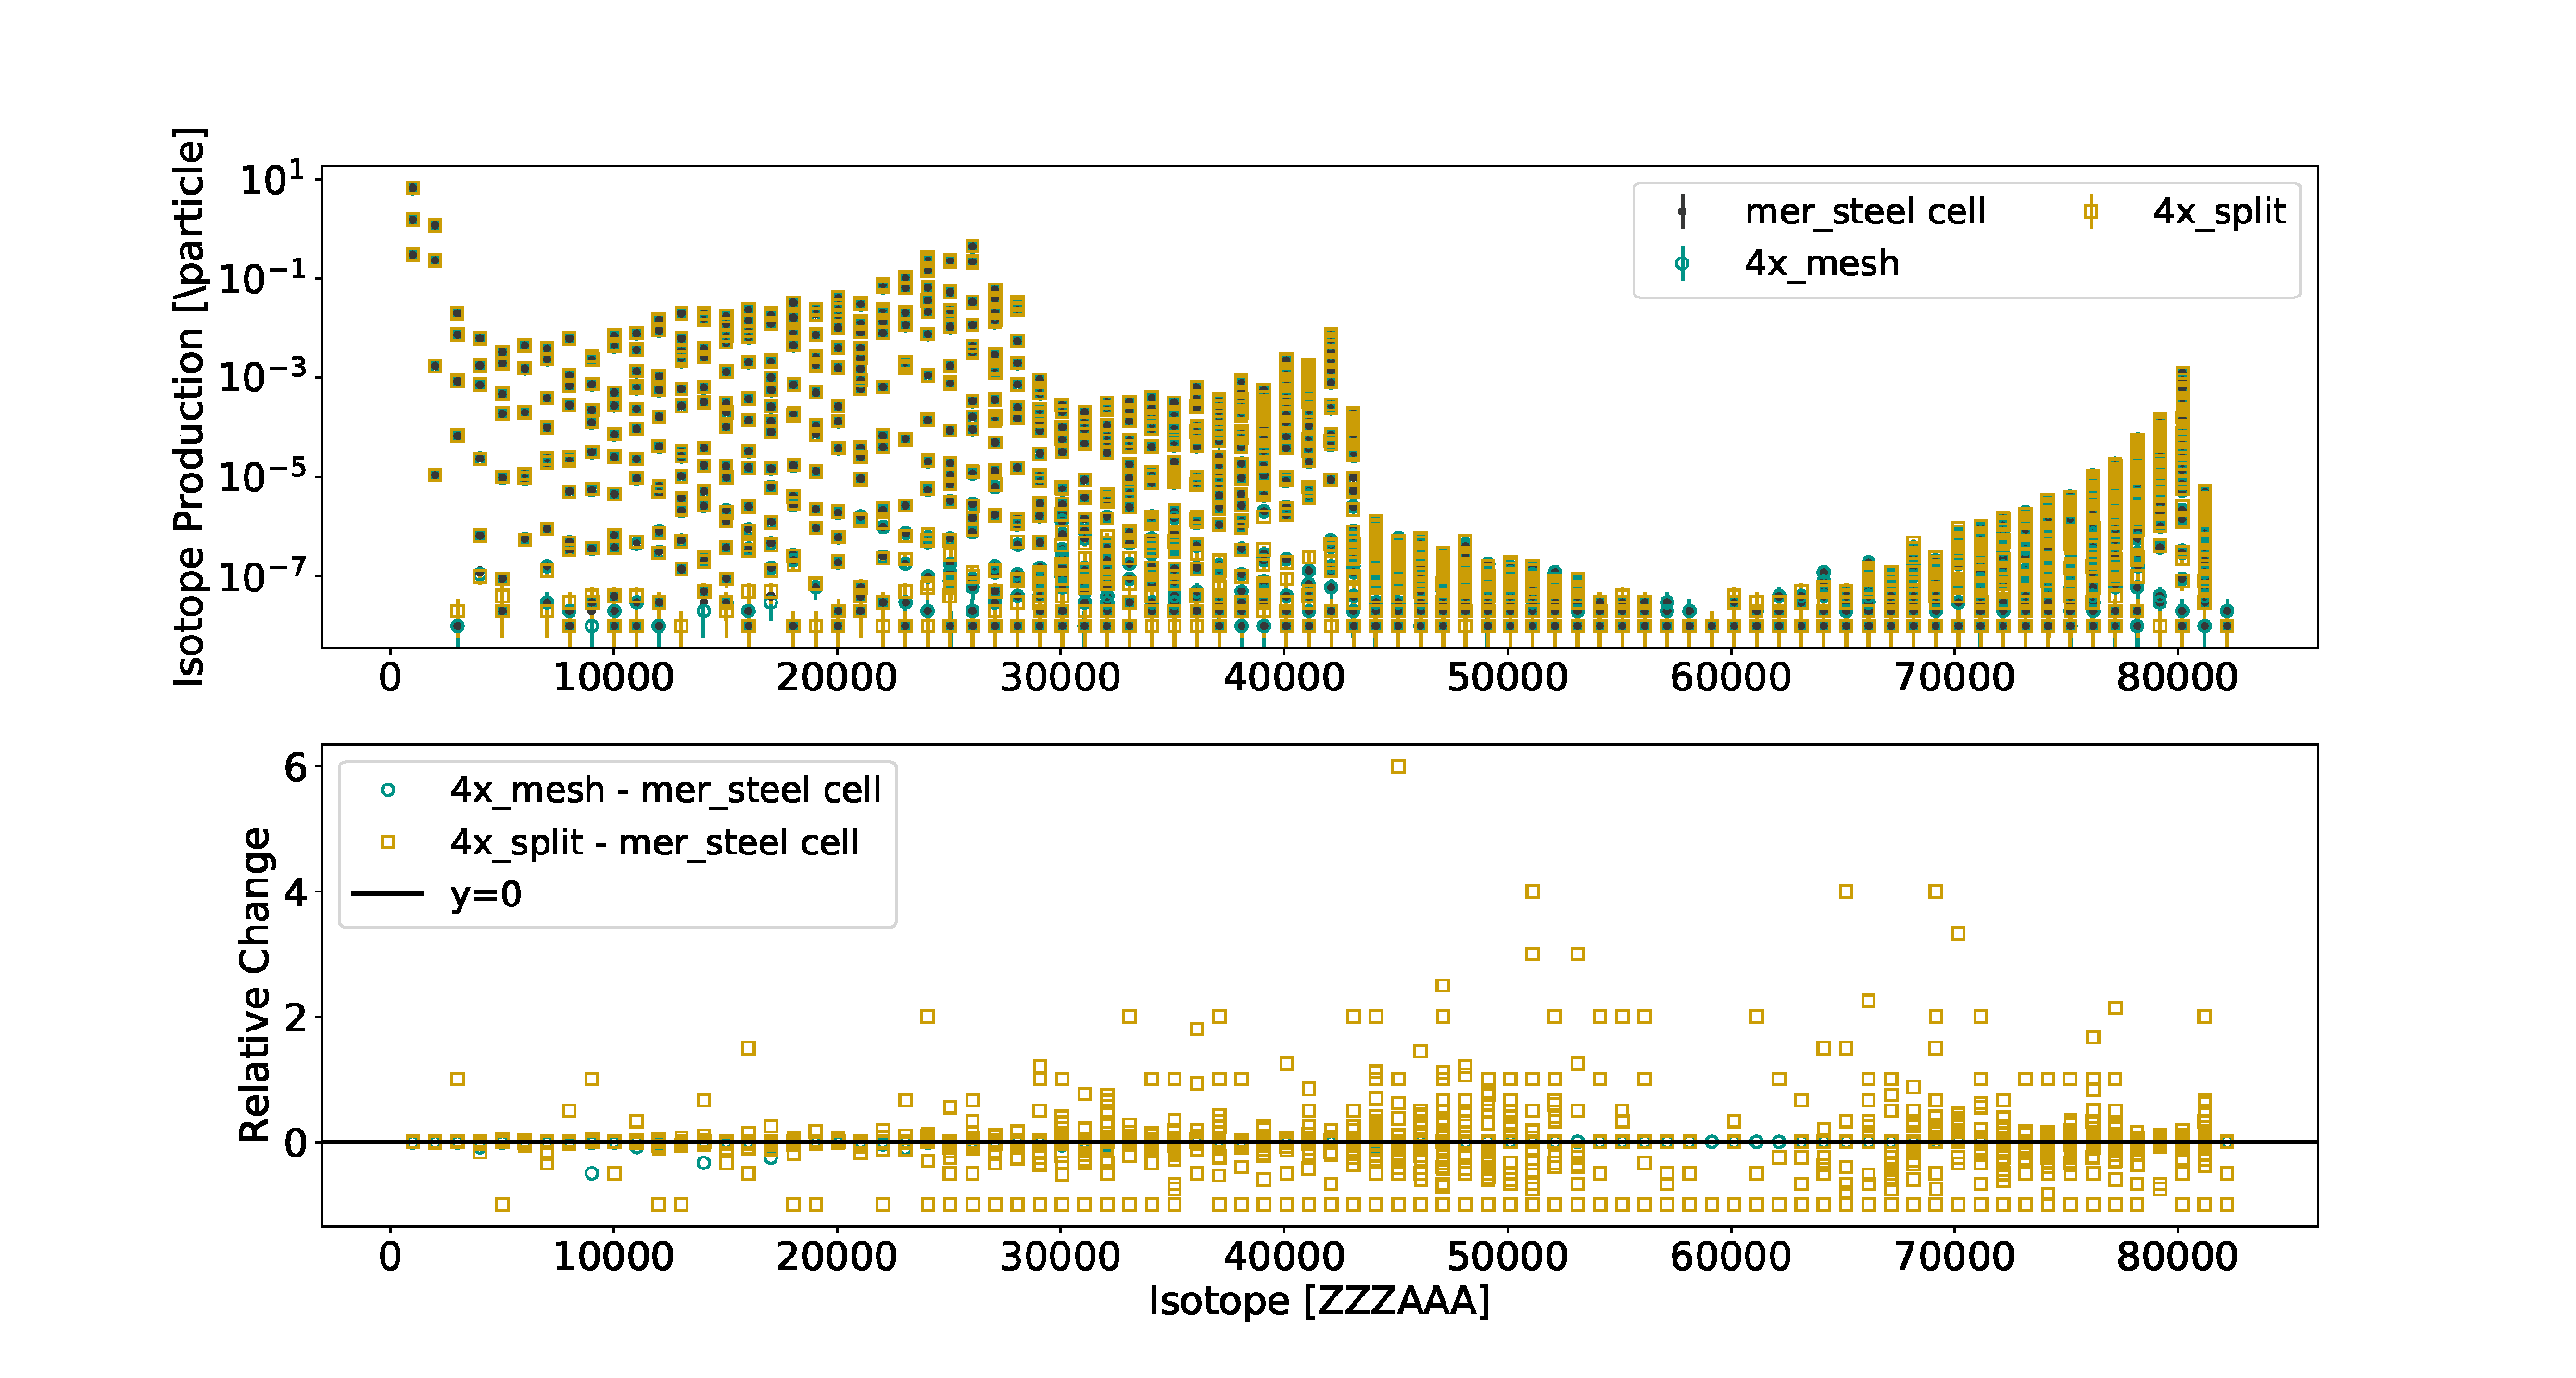
\includegraphics[scale=0.42,trim={2cm 1cm 3cm 2cm},clip]{../figs/toy_p2/prod_VPII_4x.pdf}
 \caption{Radionuclide production for mercury/steel cells, 4x4x4 mesh, and 4x4x4 divided geometry}
 \label{fig:2prod_cell_4x}
\end{figure}
%
\\
Figure \ref{fig:2prod_cell_1x_2x_4x} shows most nuclides have a small relative
change. There are a few nuclides that greater than 10\% relative change.
Figure \ref{fig:2prod_cell_2x} shows that many nuclides resulting from the
divided geometry have extremely high relative change. This is largely due to
having to mix the mercury and steel materials in the neutron transport. Lastly
Figure \ref{fig:2prod_cell_4x} shows results similar to the results obtained in
the first verification problem.
%
\begin{figure}[h!]
 \centering
 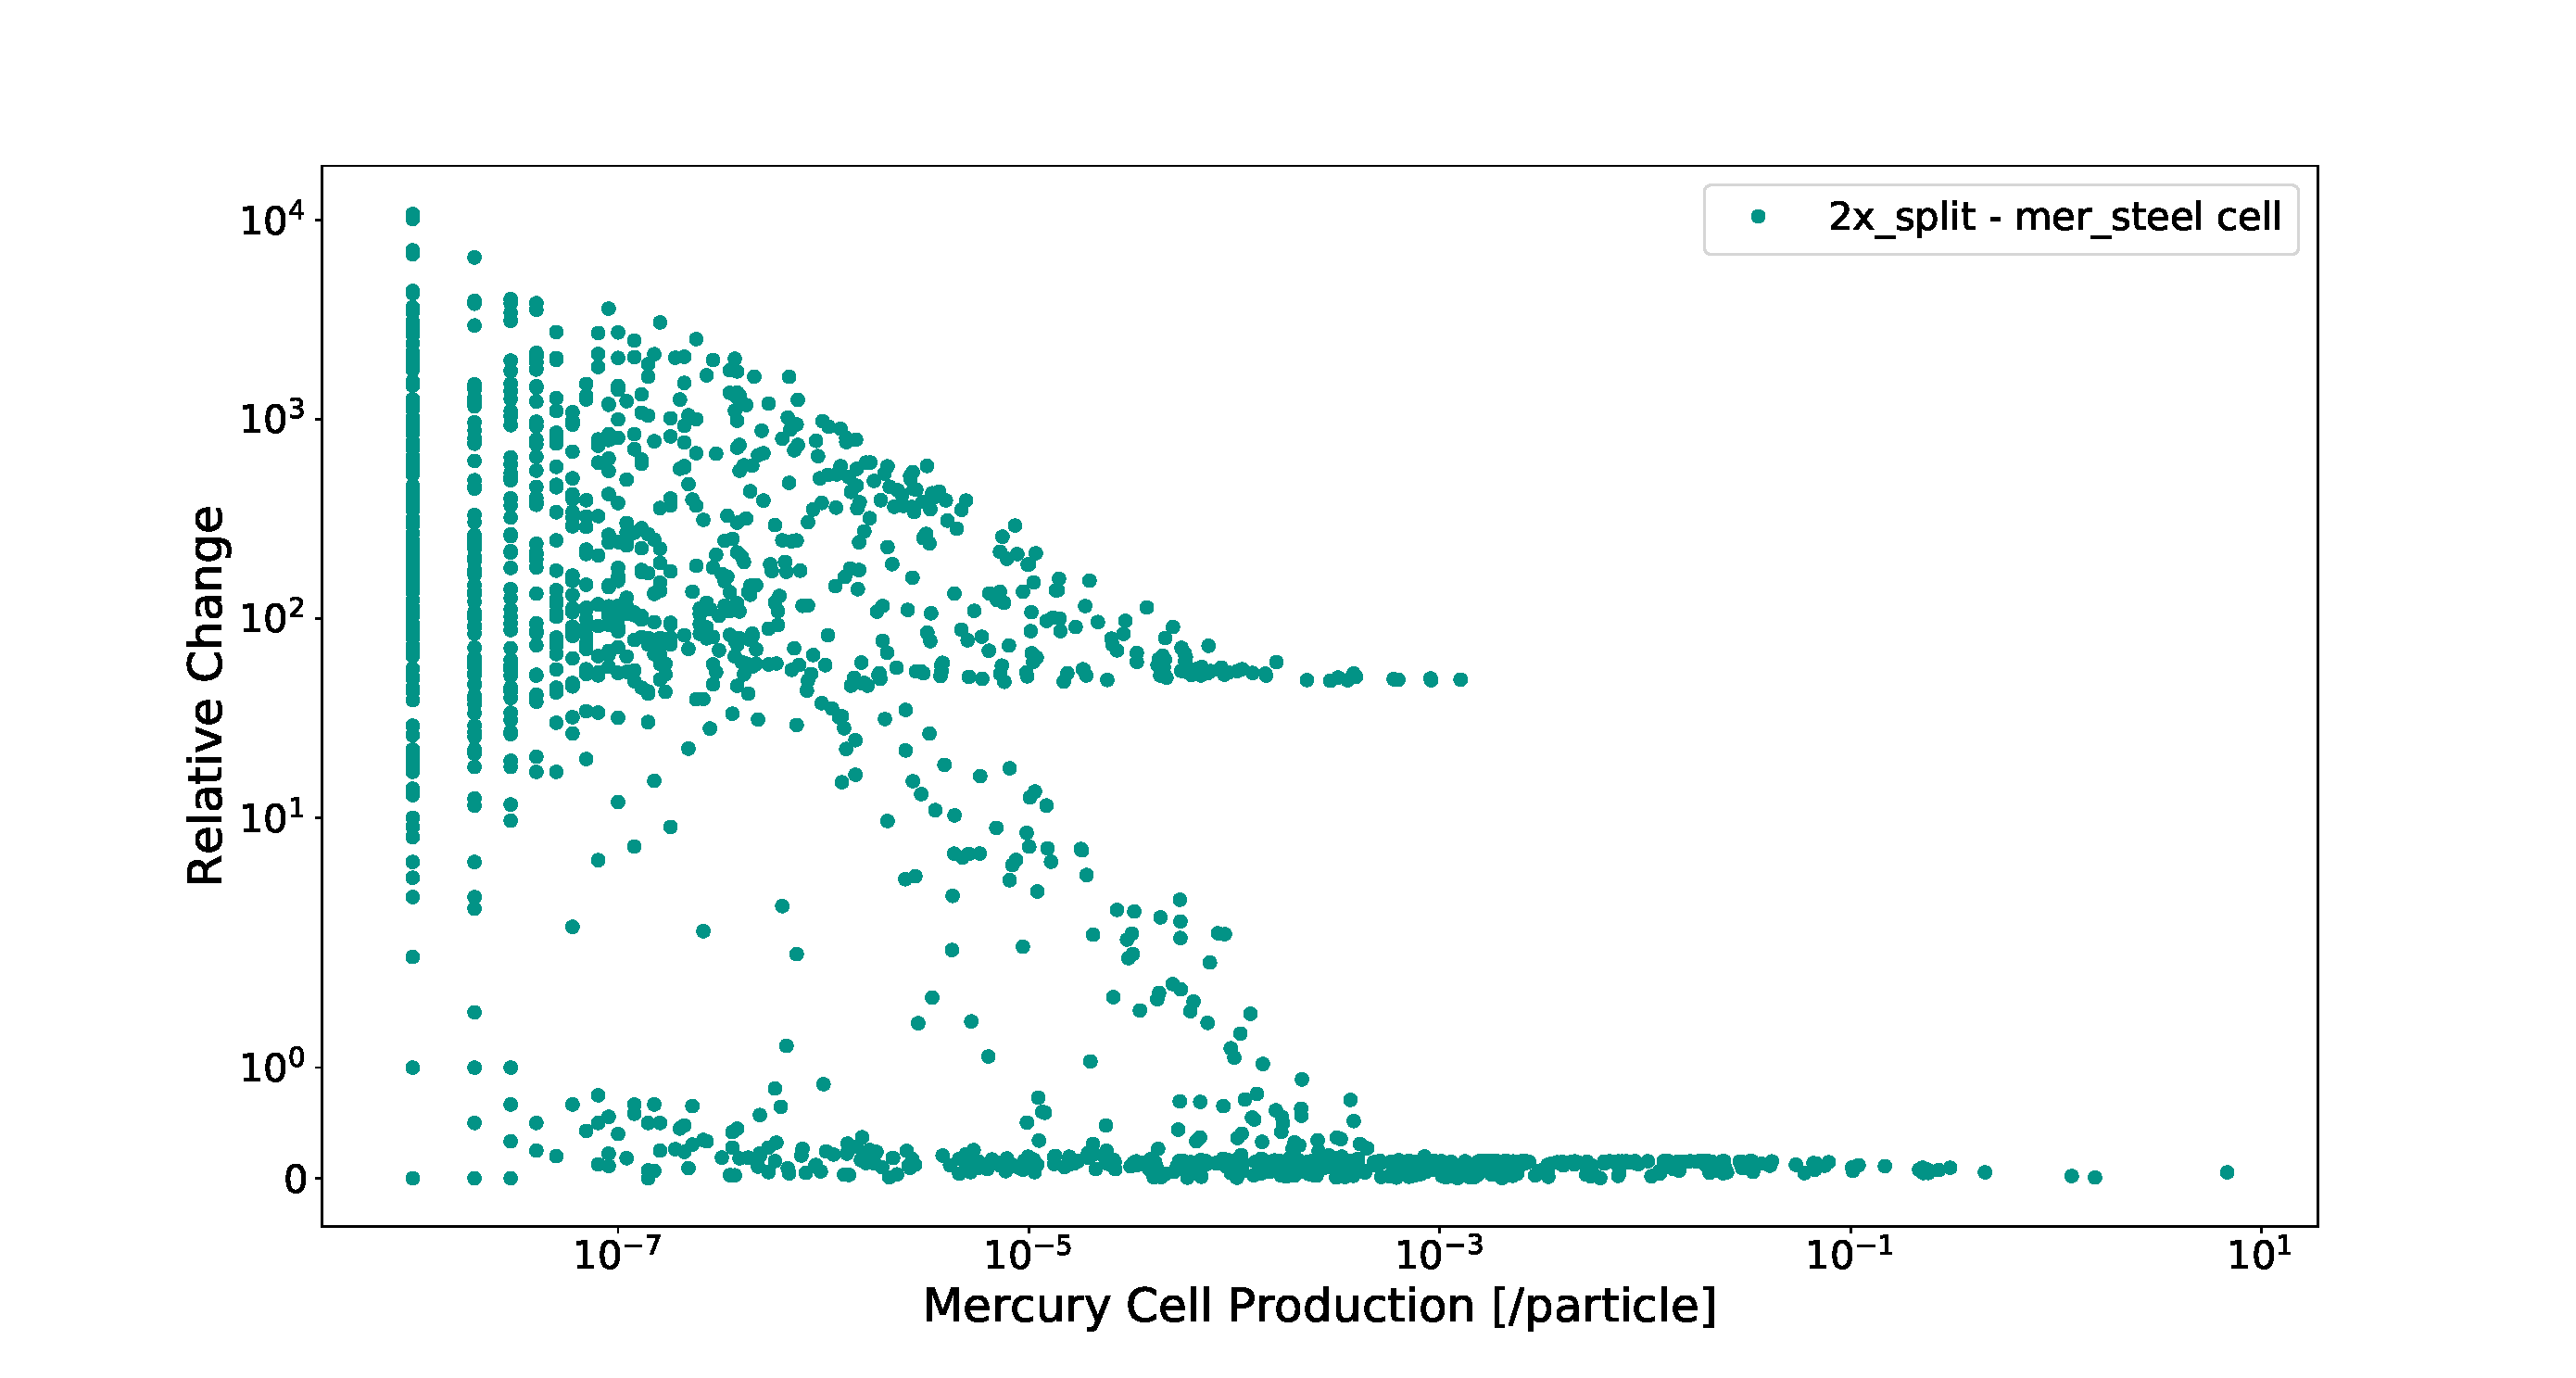
\includegraphics[scale=0.4,trim={3cm 0.5cm 3cm 3cm},clip]{../figs/toy_p2/prod_VPII_rc_2x_split.pdf}
 \caption{Relative change between cell method and 2x2x2 geometry split vs. the isotope production of the mercury cell}
 \label{fig:2prod_cell_2x_rc}
\end{figure}
\begin{figure}[h!]
 \centering
 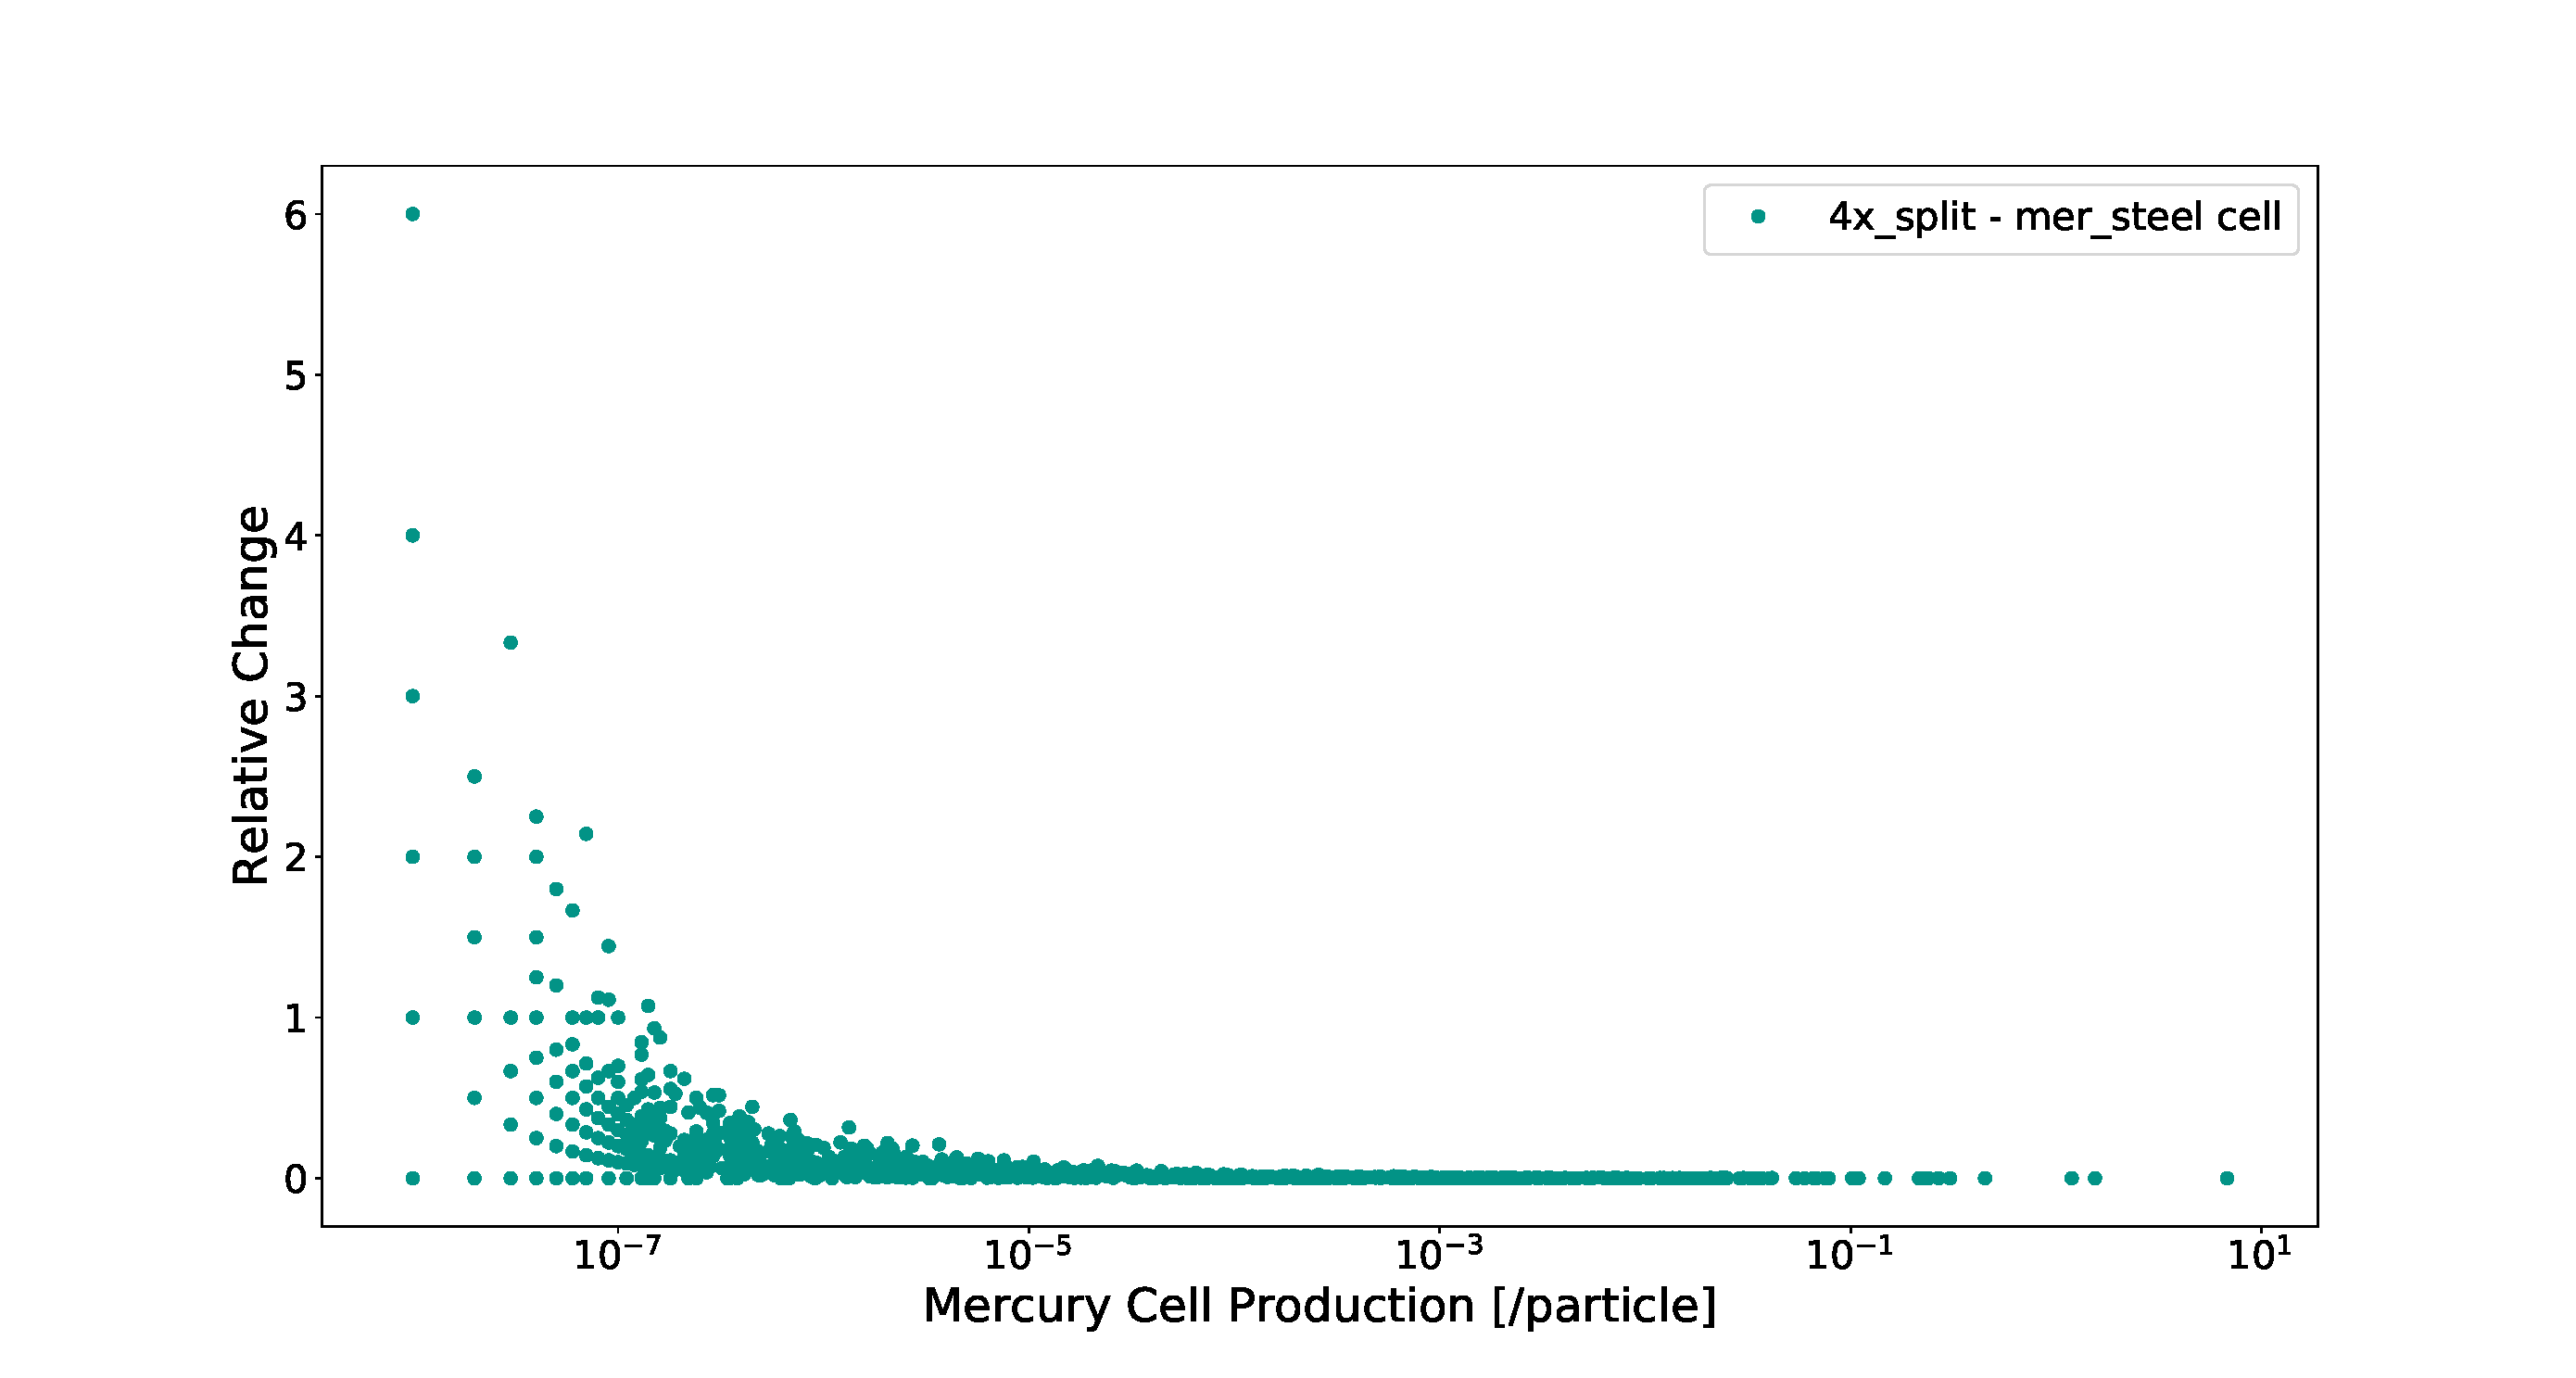
\includegraphics[scale=0.4,trim={3cm 0.5cm 3cm 3cm},clip]{../figs/toy_p2/prod_VPII_rc_4x_split.pdf}
 \caption{Relative change between cells and 4x4x4 geometry split vs. the isotope production of the mercury cell}
 \label{fig:2prod_cell_4x_rc}
\end{figure}
%
\\
\begin{figure}[h!]
 \centering
 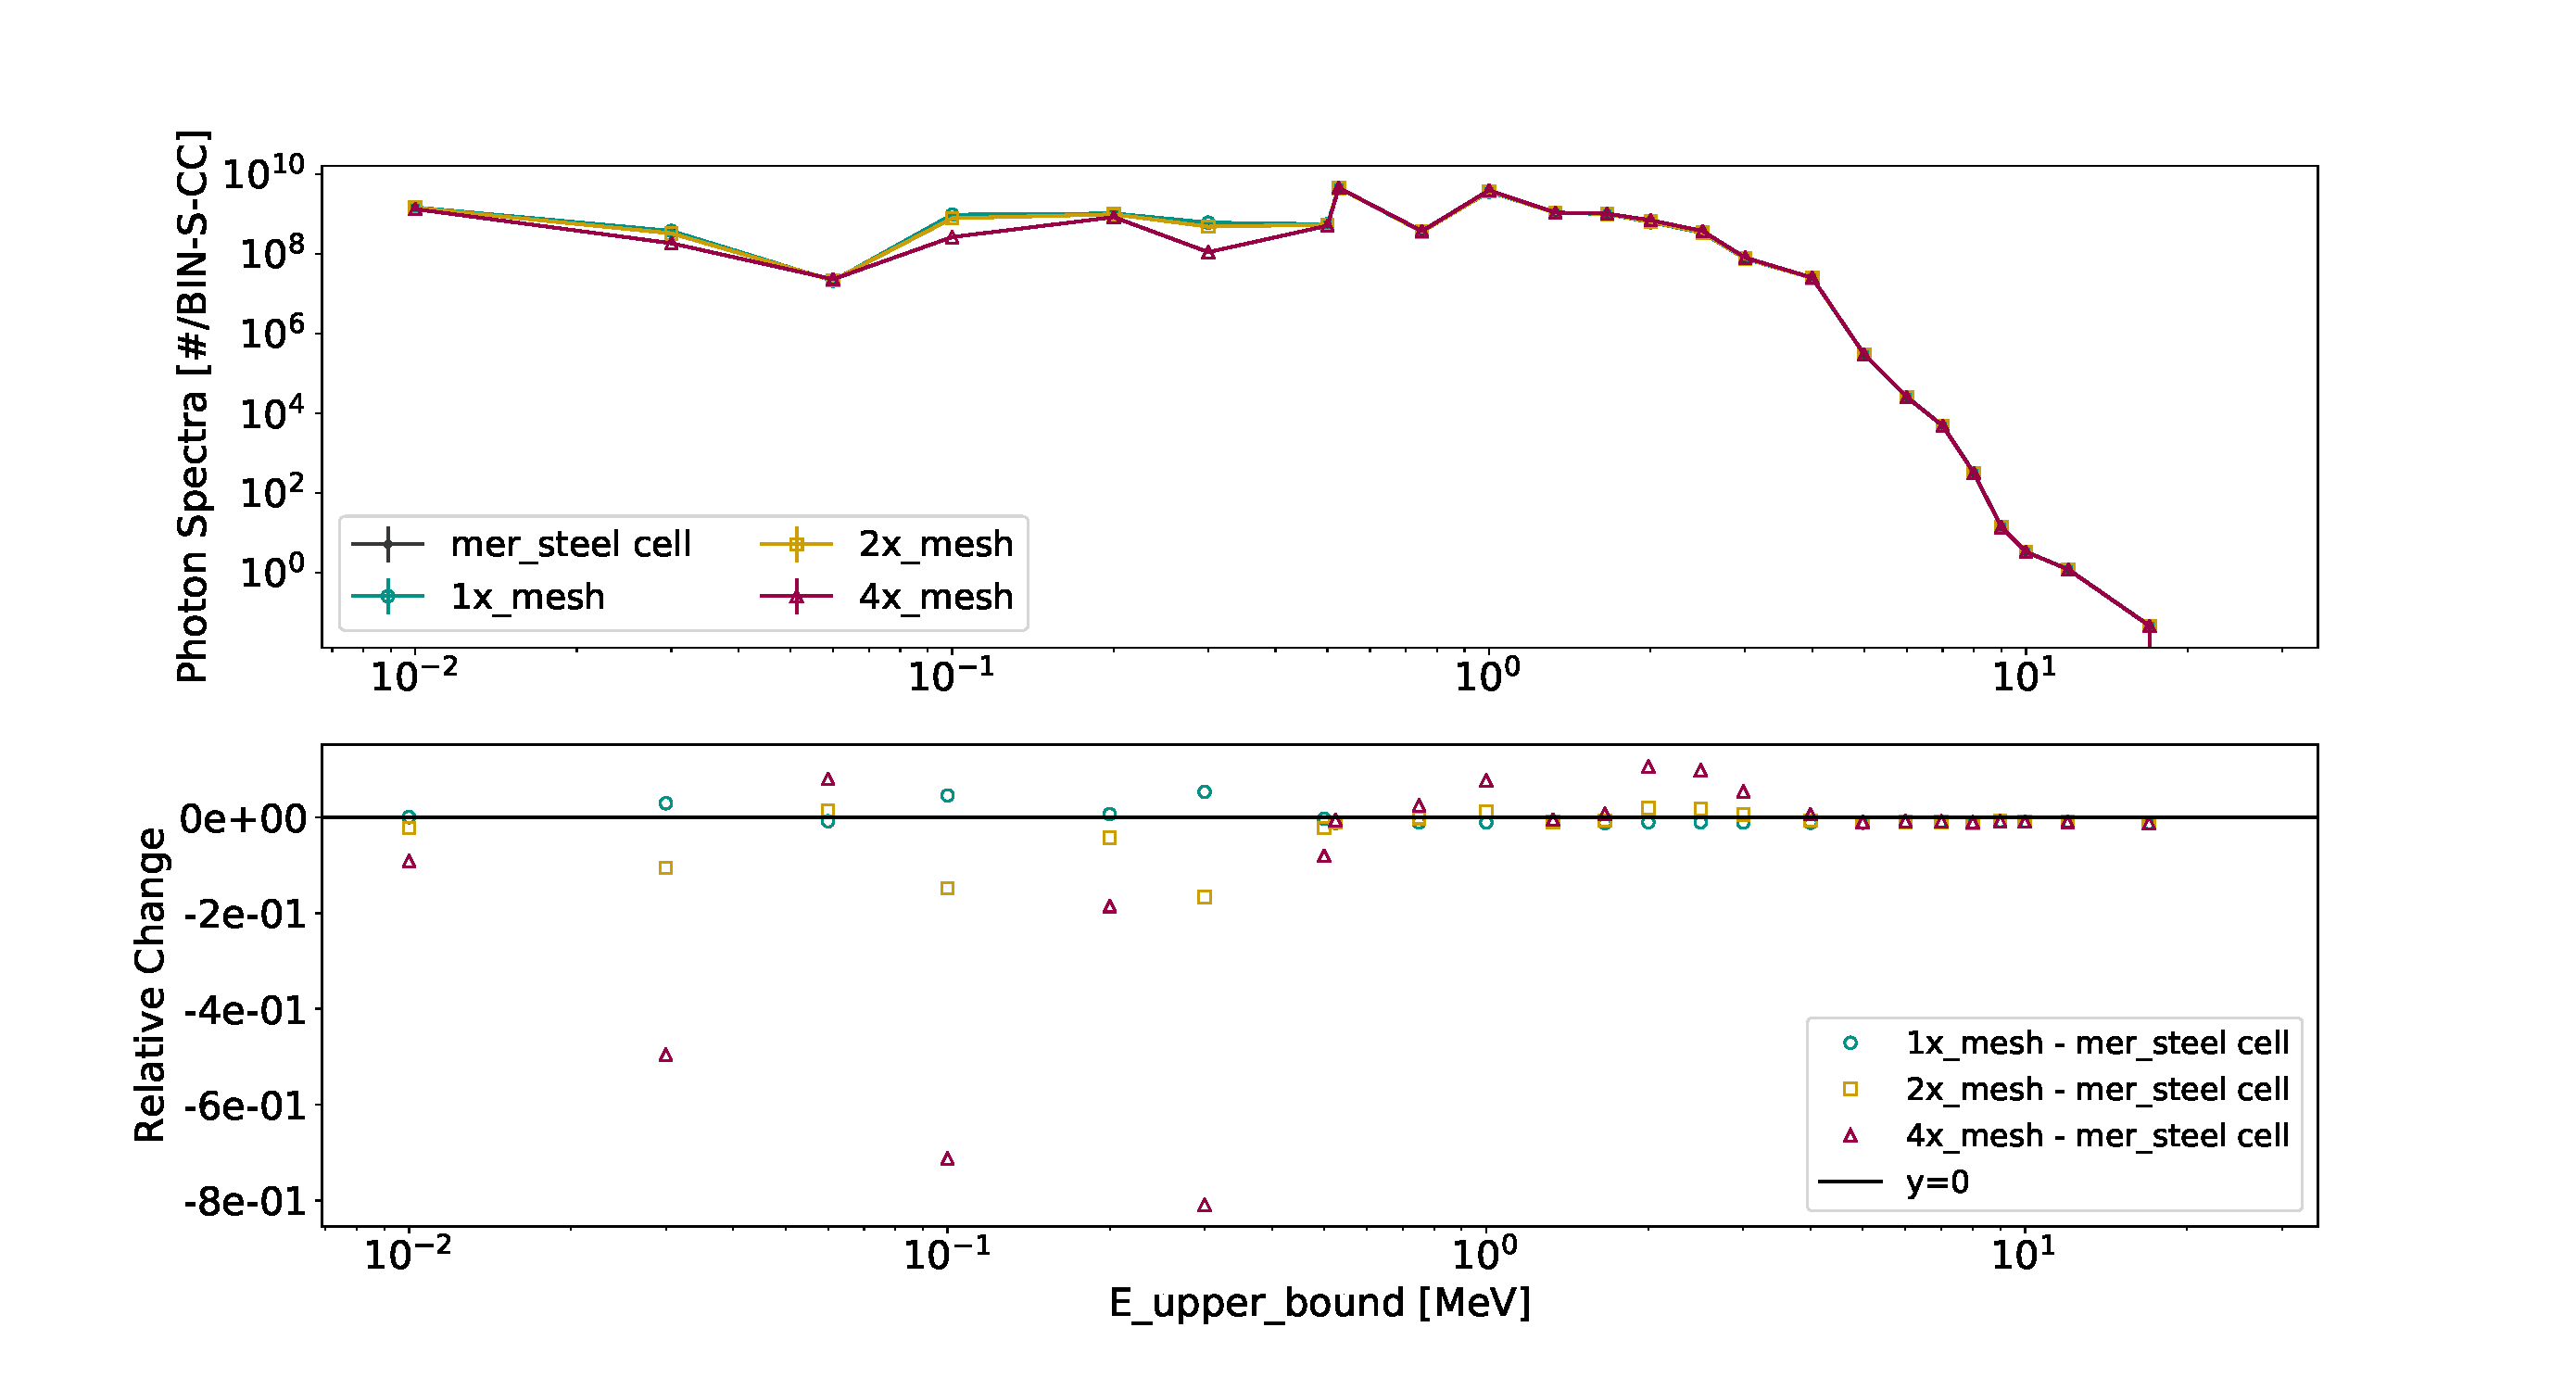
\includegraphics[scale=0.42,trim={2cm 0.5cm 3cm 2cm},clip]{../figs/toy_p2/spec_VPII_1x_2x_4x.pdf}
 \caption{Photon Spectrum in mercury/steel cell and different meshes}
 \label{fig:2spec_cell_1x_2x_4x}
\end{figure}
%
A comparison between the results in the mesh and the split geometry can be seen
in Figure \ref{fig:2spec_cell_2x} and \ref{fig:2spec_cell_4x}.
%
\begin{figure}[h!]
 \centering
 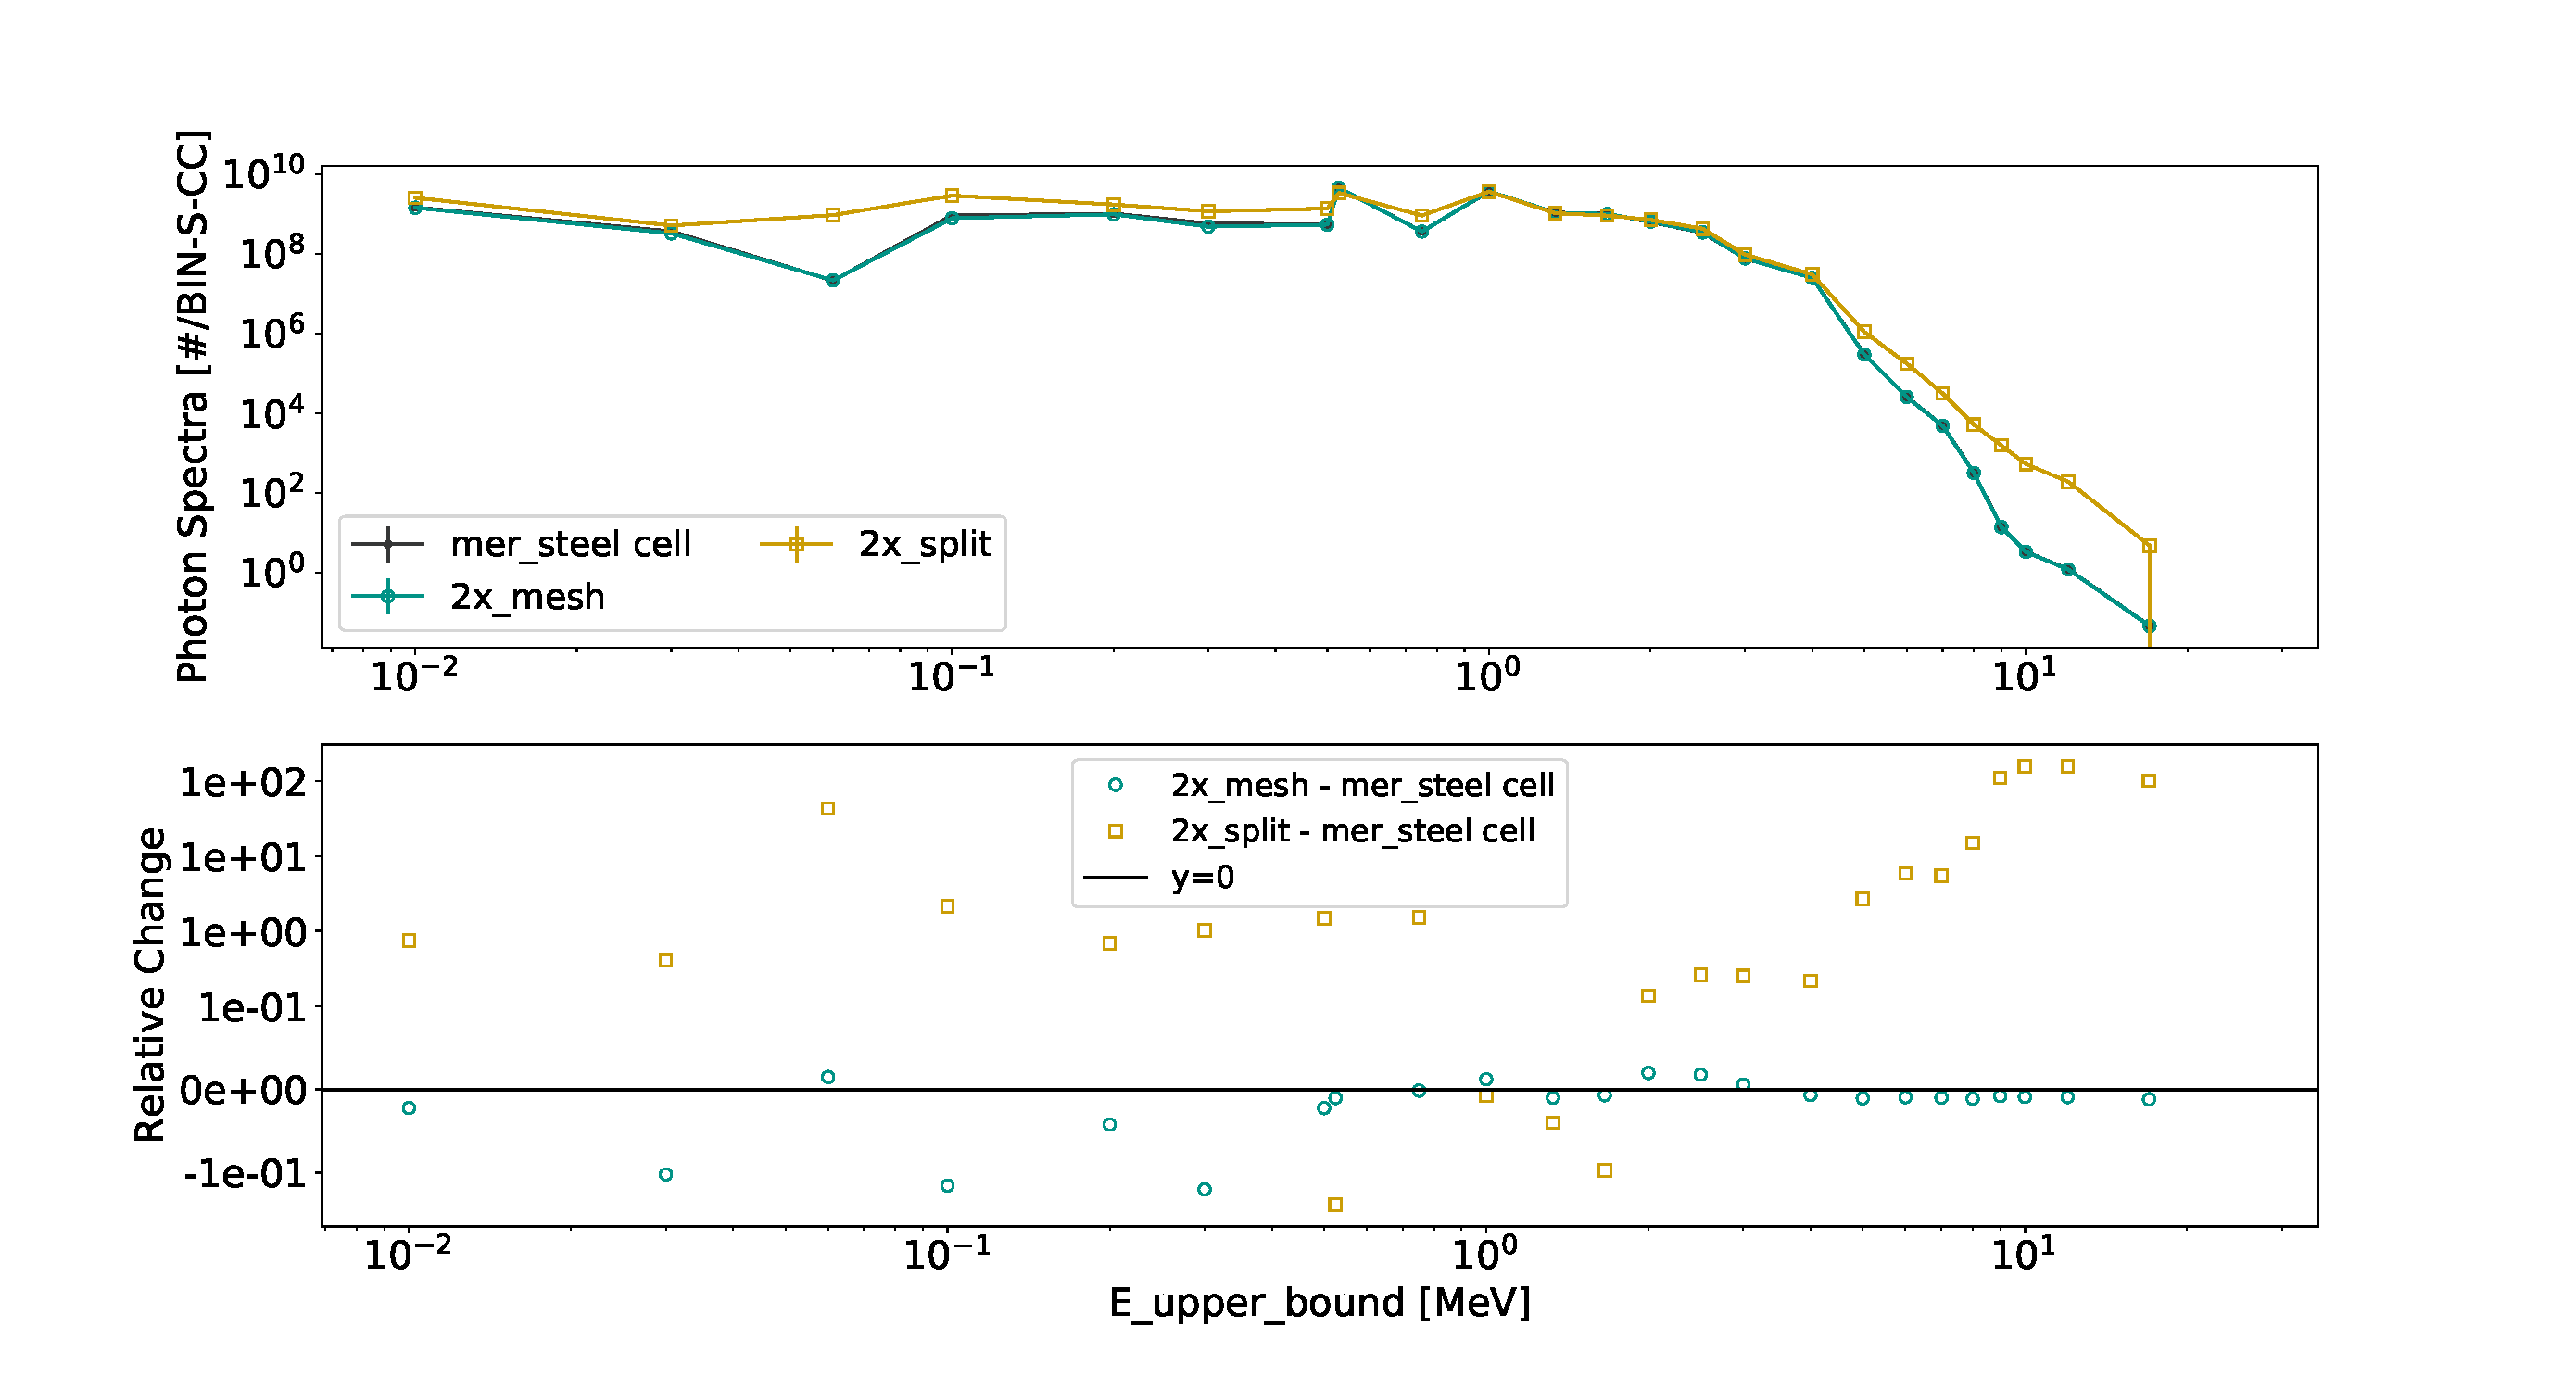
\includegraphics[scale=0.42,trim={2cm 0.5cm 3cm 2cm},clip]{../figs/toy_p2/spec_VPII_2x.pdf}
 \caption{Photon Spectrum in mercury cell, 2x2x2 mesh, and geometry split}
 \label{fig:2spec_cell_2x}
\end{figure}
%
\begin{figure}[h!]
 \centering
 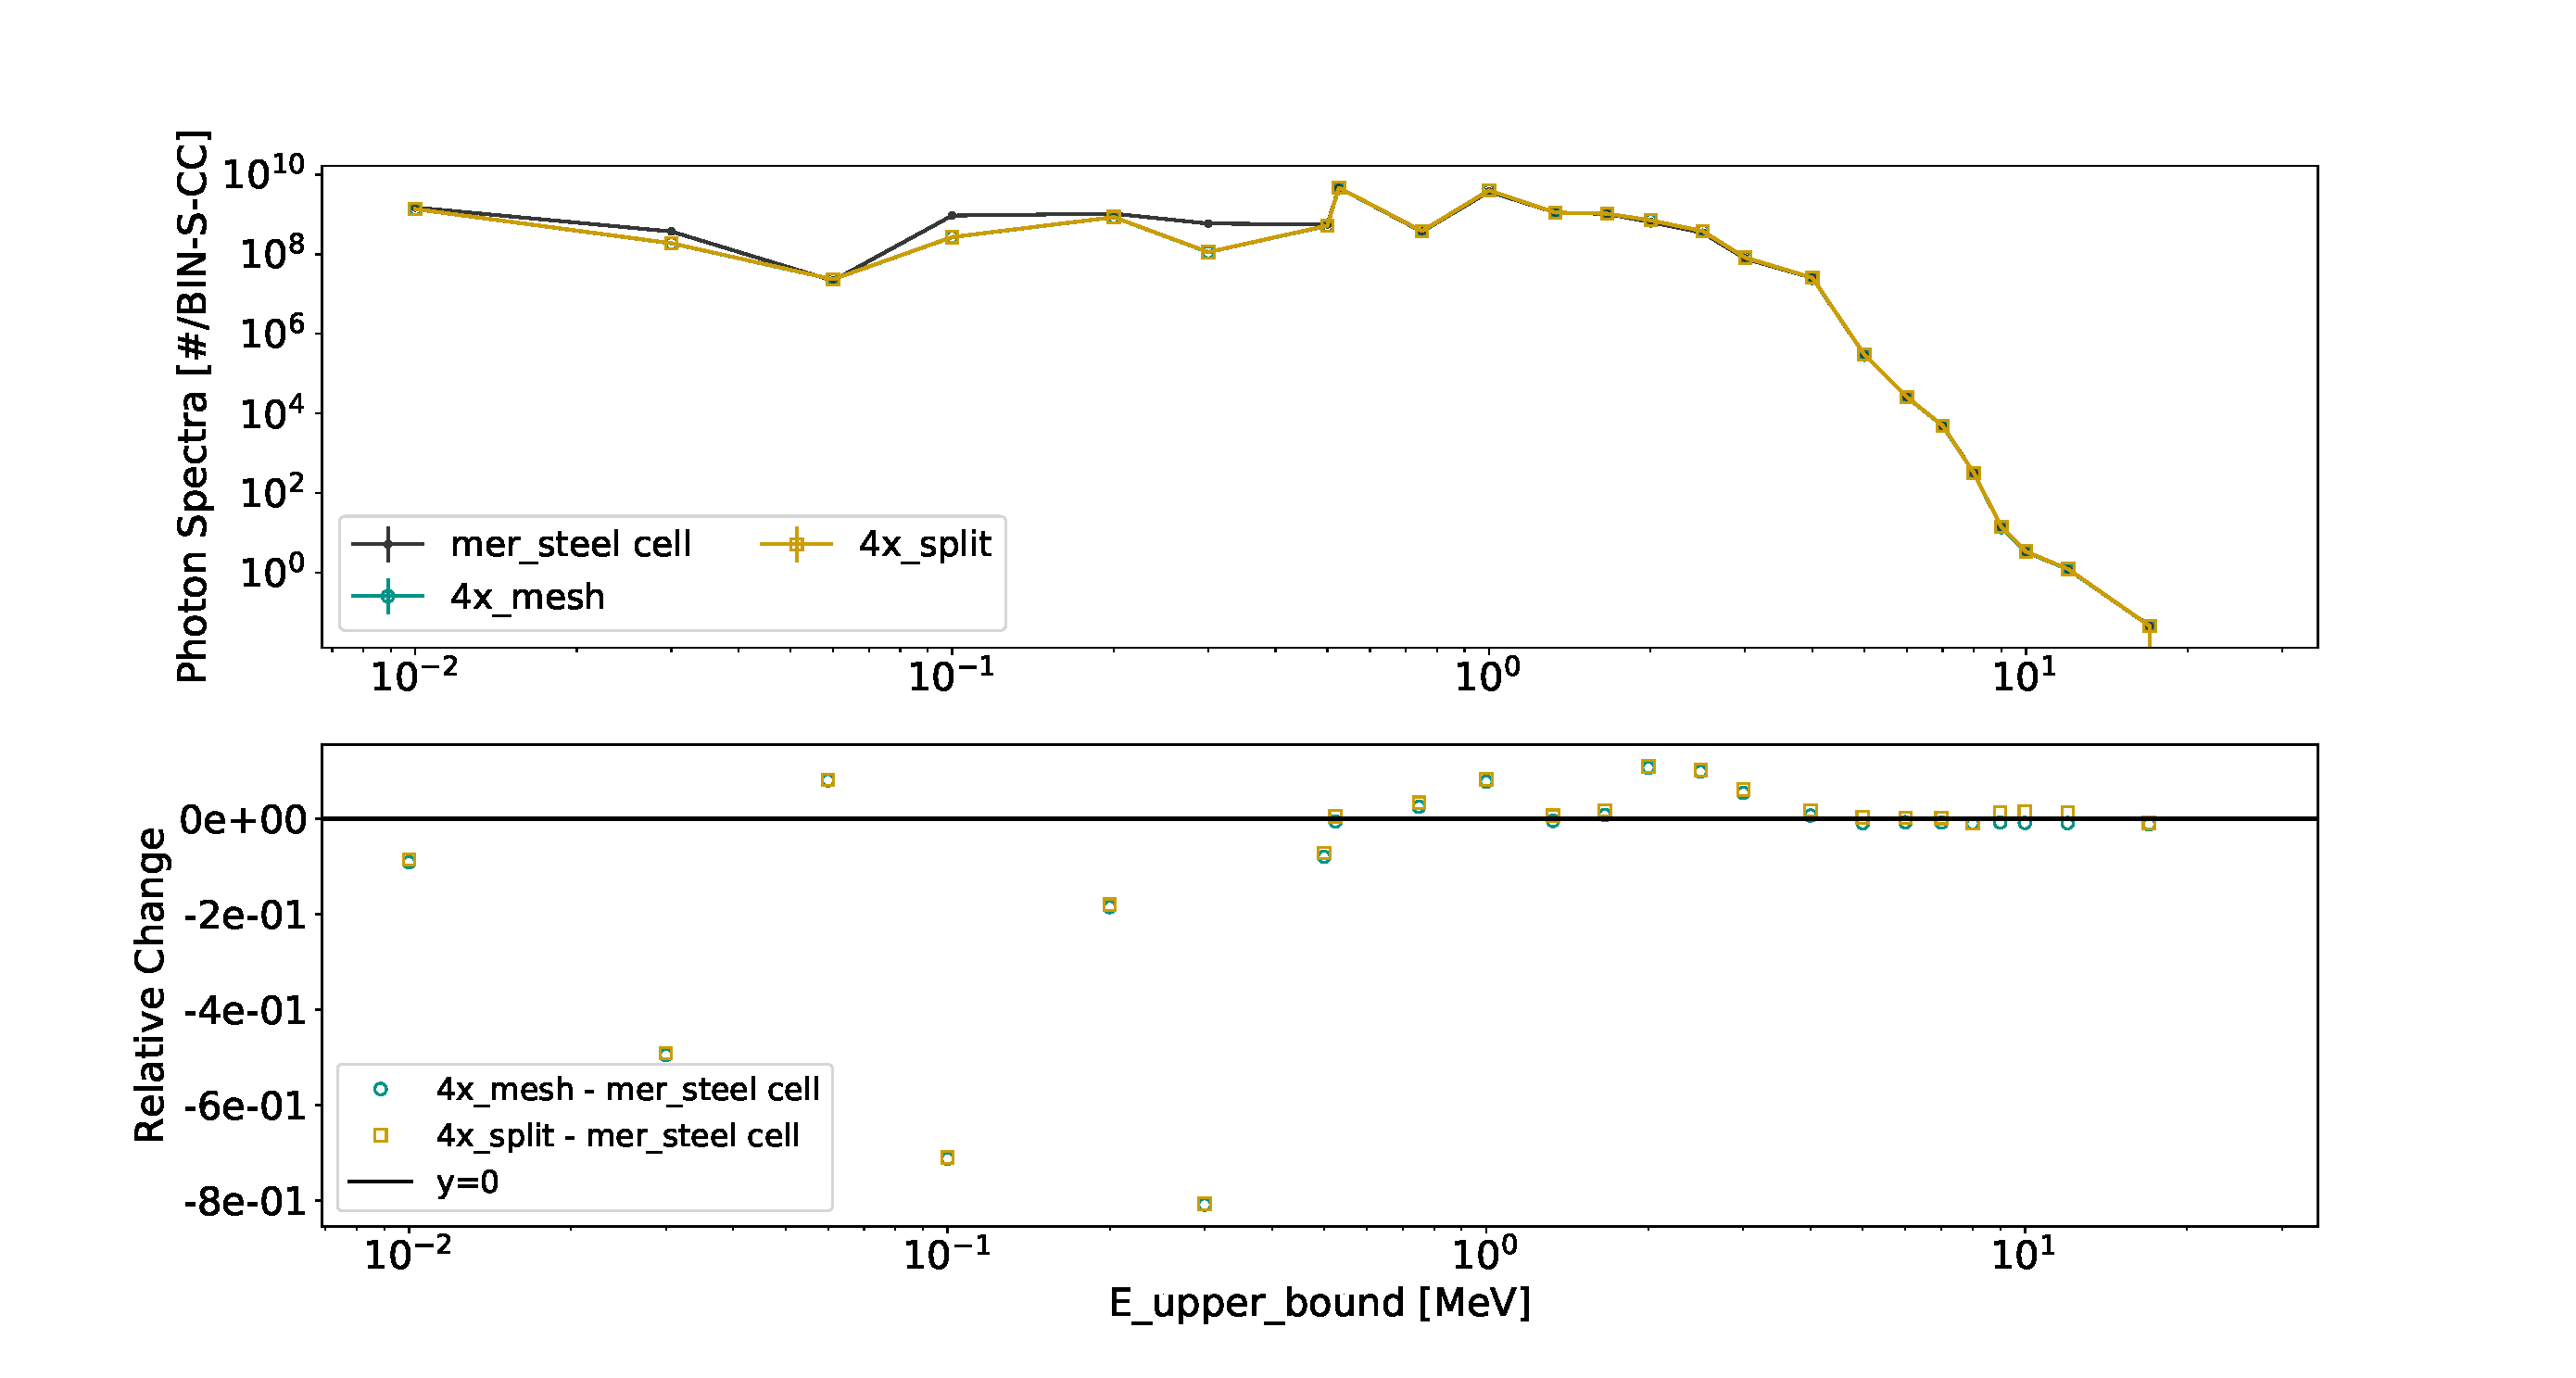
\includegraphics[scale=0.42,trim={2cm 0.5cm 3cm 2cm},clip]{../figs/toy_p2/spec_VPII_4x.pdf}
 \caption{Photon Spectrum in mercury/steel cell, 4x4x4 mesh, and geometry split}
 \label{fig:2spec_cell_4x}
\end{figure}
%


Figure \ref{fig:2spec_8v} shows the results per voxel for a 2x2x2 mesh.
\begin{figure}
	\centering
	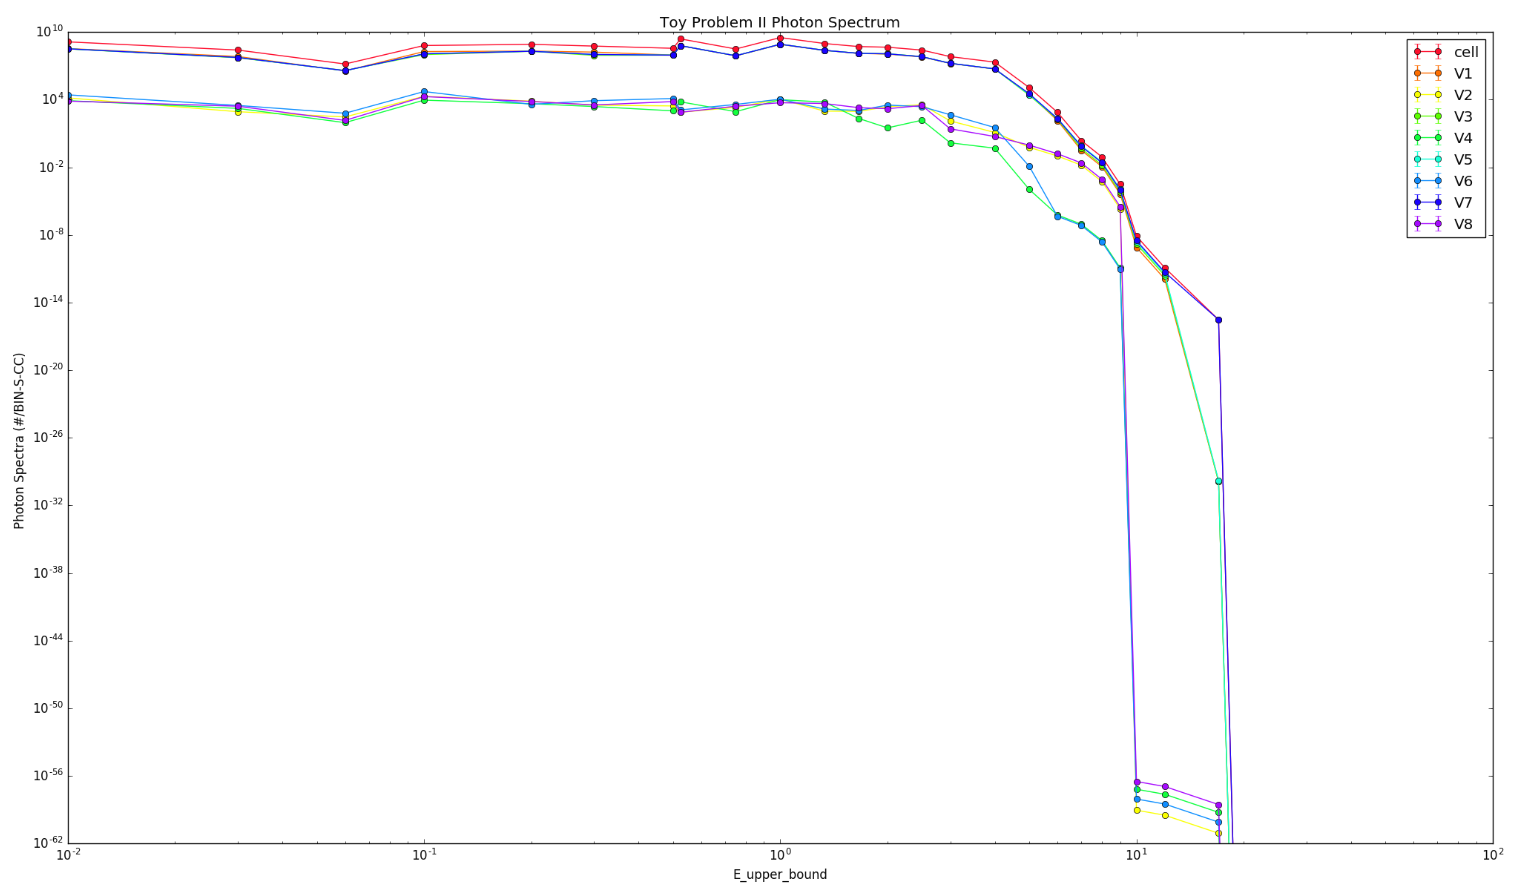
\includegraphics[scale=0.3, trim={0cm 0cm 0cm 1cm},clip]{../figs/toy_p2/spec_VPII_8.png}
	\caption{No sure}
	\label{fig:2spec_8v}
\end{figure}
\\
The biological dose was then calculated using the photon emission density.
Figures \ref{fig:2dose}
%
\begin{figure}
	\begin{subfigure}[t]{0.5\textwidth}
		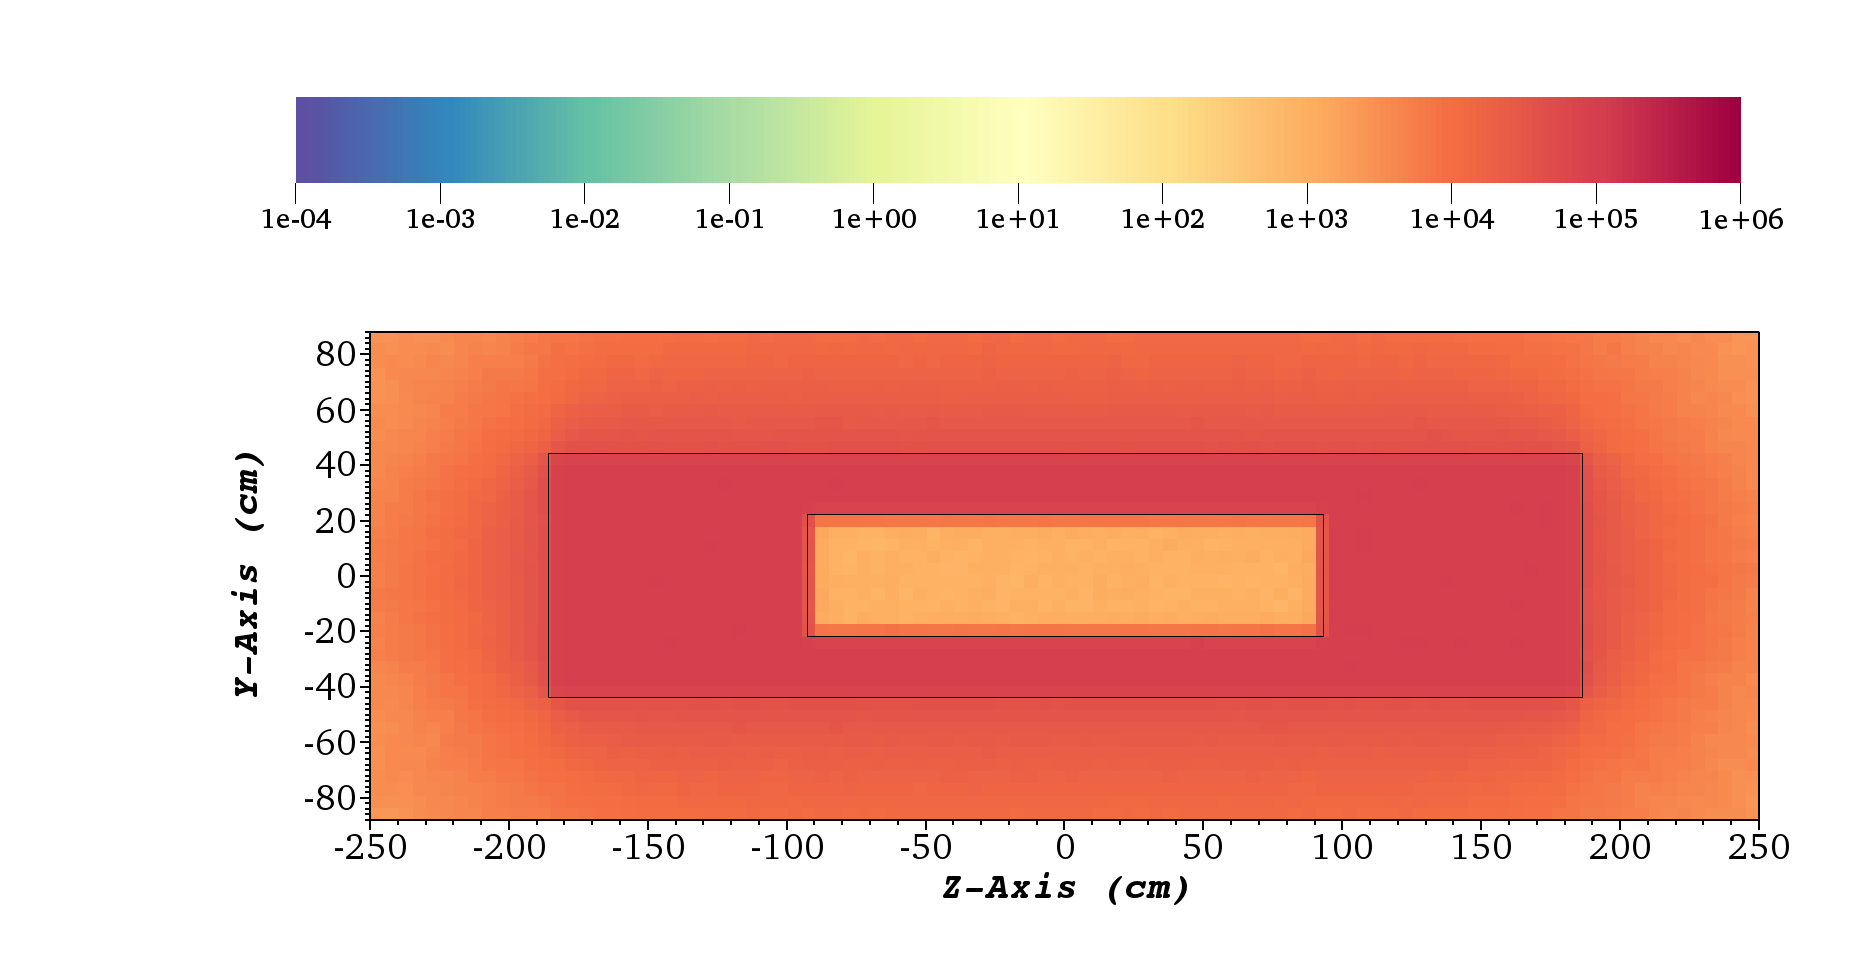
\includegraphics[width=\linewidth, trim={8cm 2cm 2cm 10cm},clip]{../figs/toy_p2/dose_VPII_original.png}
		\caption{full geometry}
		\label{fig:2dose_orig}
	\end{subfigure}\hfill
	\begin{subfigure}[t]{0.5\textwidth}
		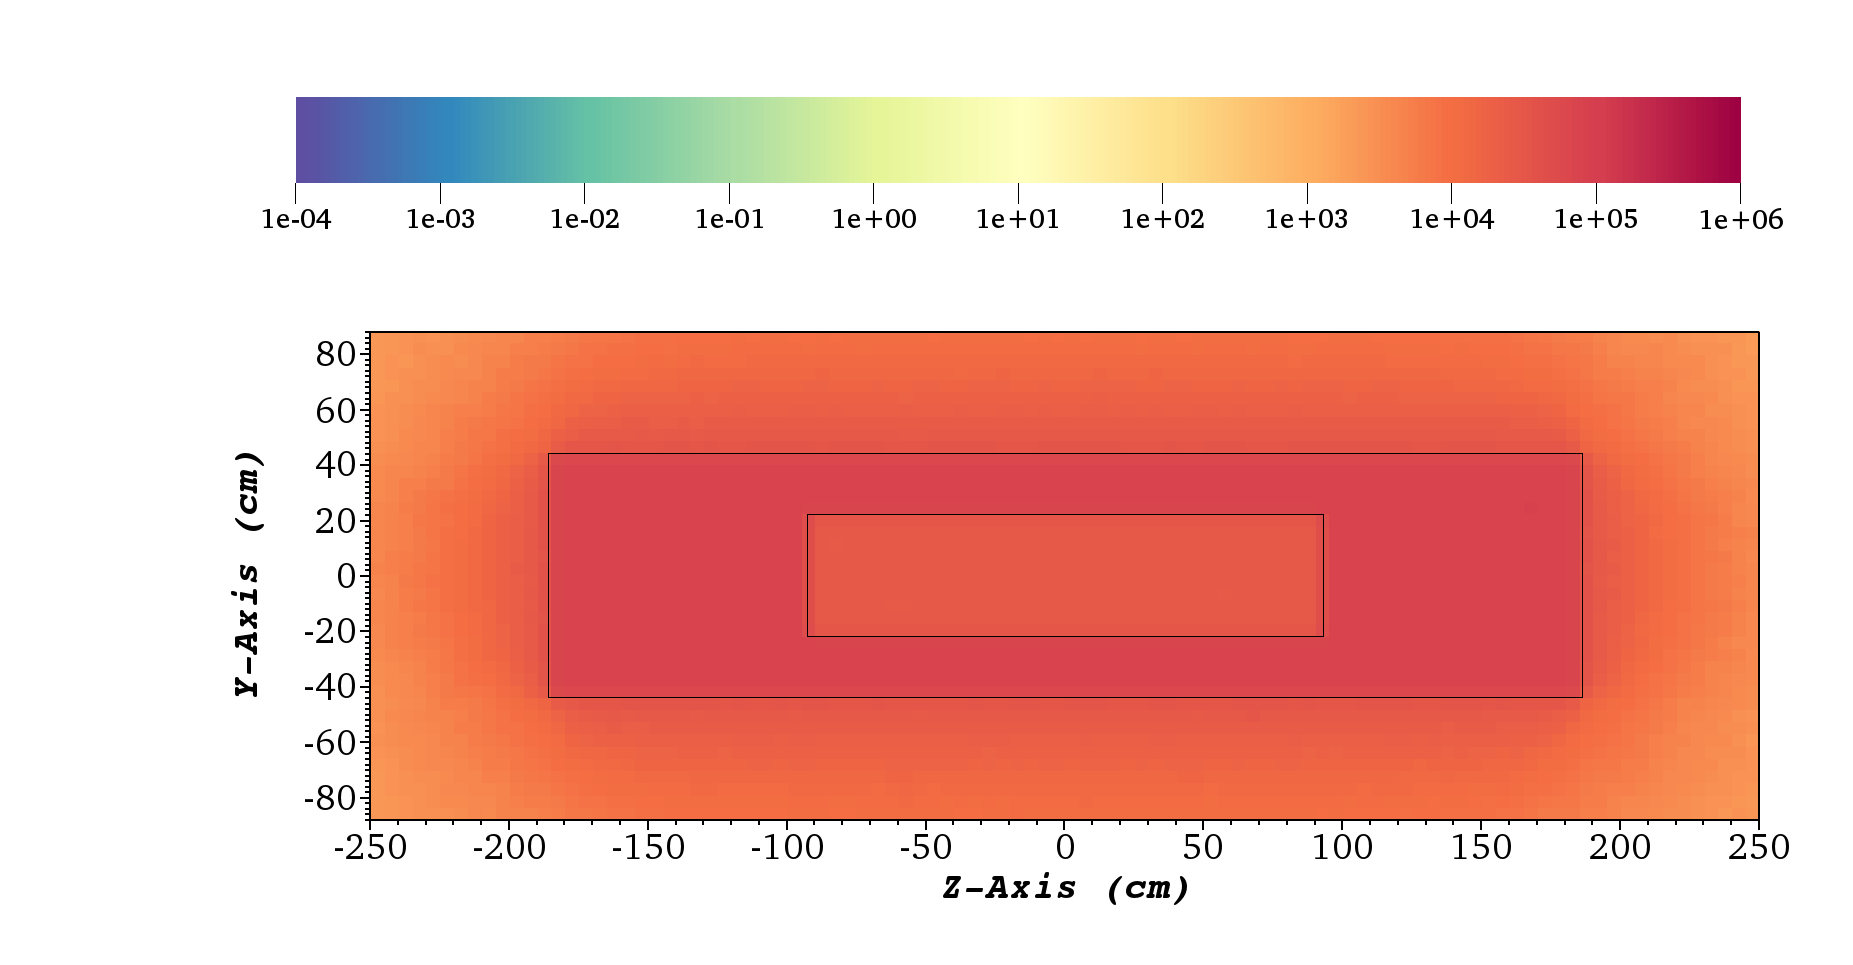
\includegraphics[width=\linewidth, trim={8cm 2cm 2cm 10cm},clip]{../figs/toy_p2/dose_VPII_1x_mesh.png}
		\caption{1x1x1 mesh}
		\label{fig:2dose_1x_mesh}
	\end{subfigure}

	\begin{subfigure}[t]{0.5\textwidth}
		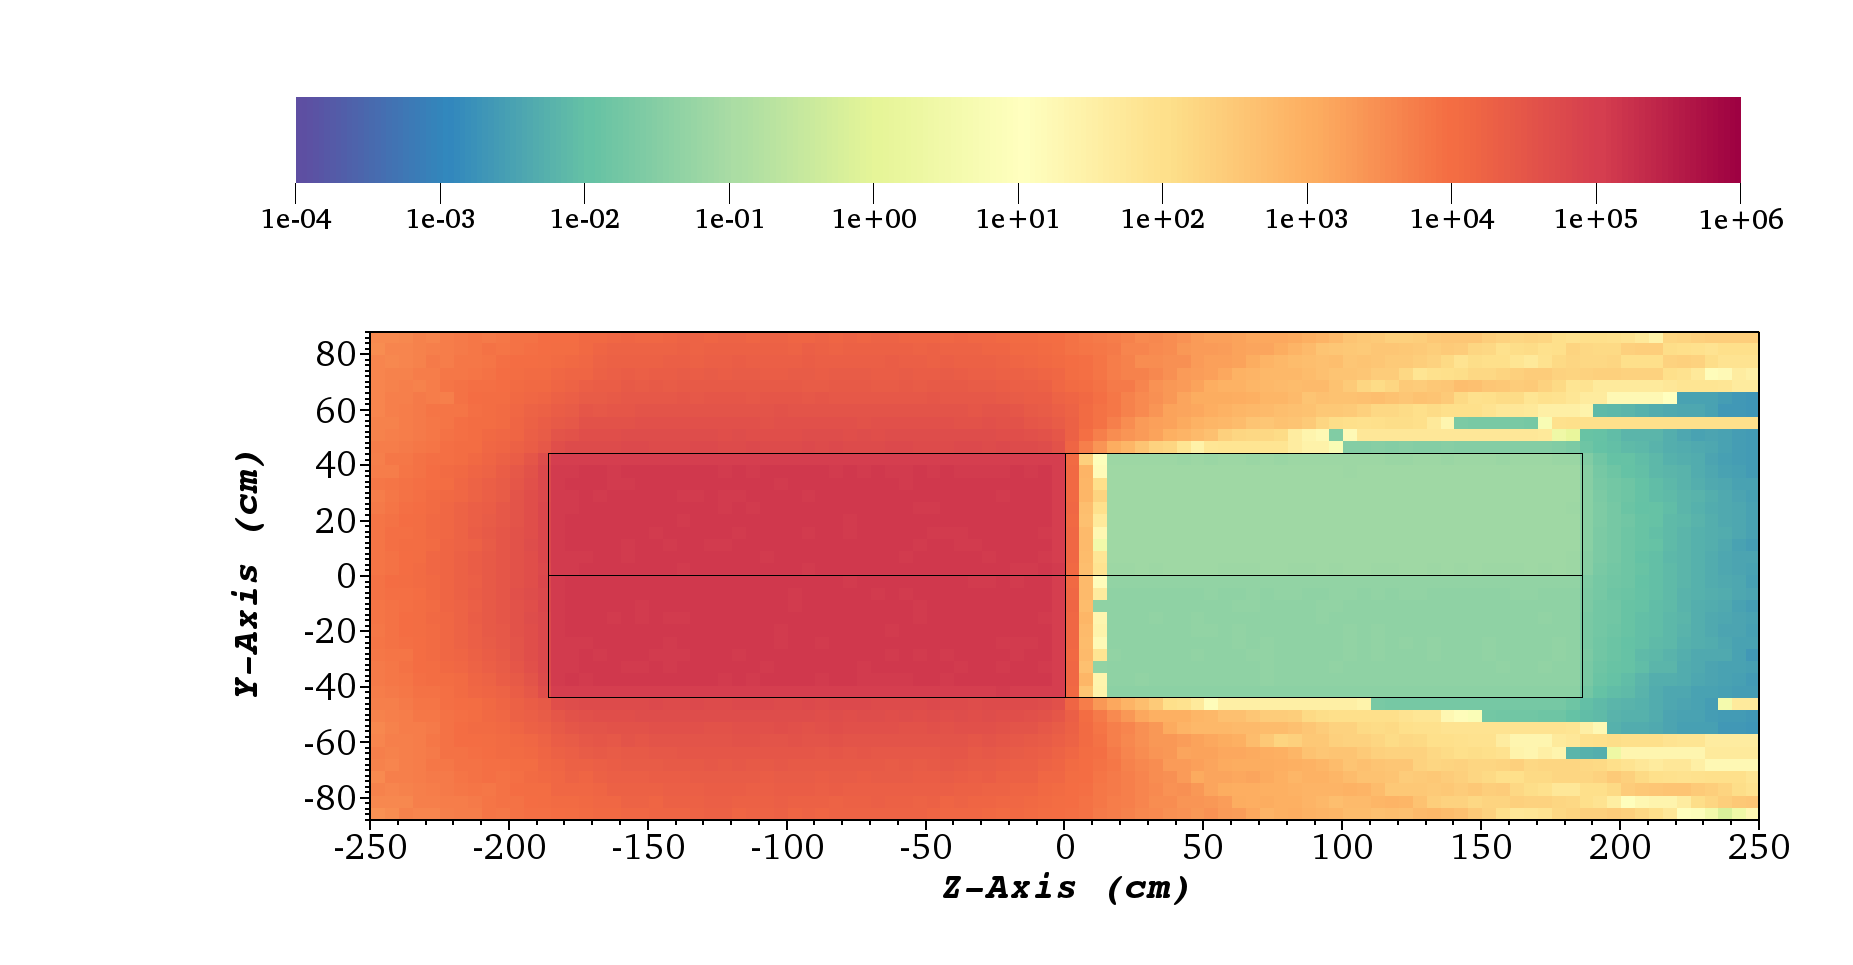
\includegraphics[width=\linewidth, trim={8cm 2cm 2cm 10cm},clip]{../figs/toy_p2/dose_VPII_2x_split.png}
		\caption{2x2x2 divided}
		\label{fig:2dose_2x_split}
	\end{subfigure}\hfill
	\begin{subfigure}[t]{0.5\textwidth}
		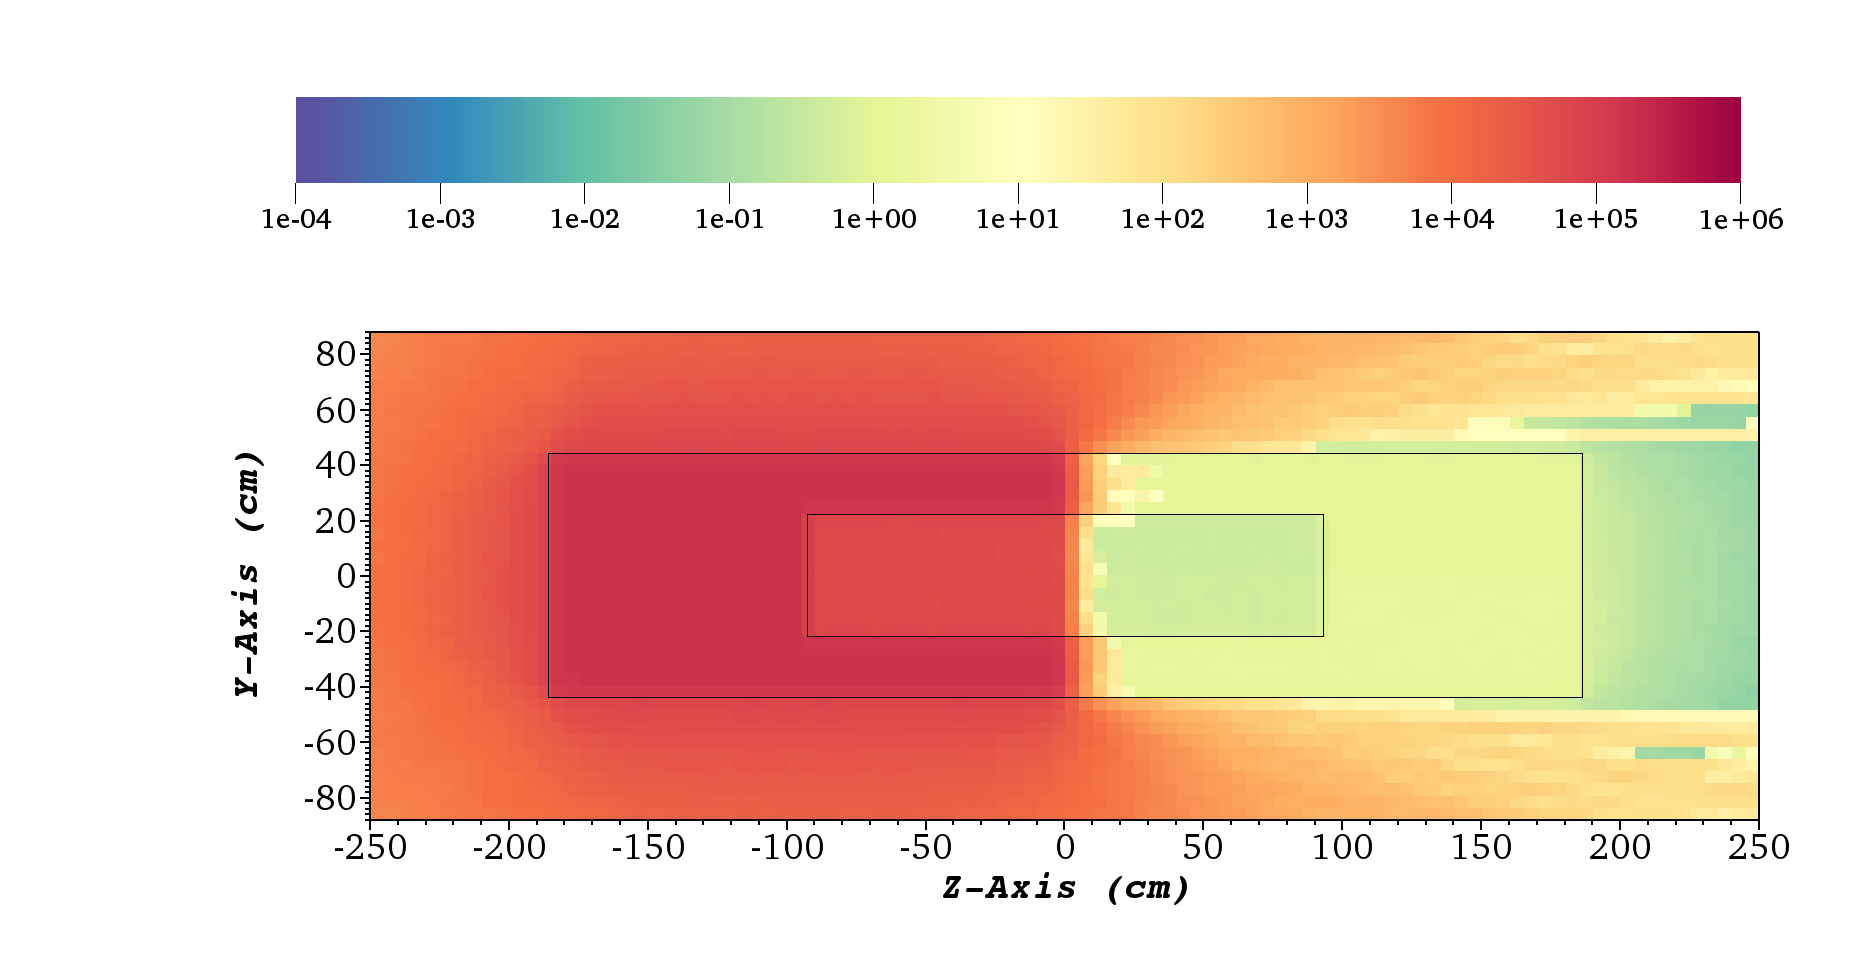
\includegraphics[width=\linewidth, trim={8cm 2cm 2cm 10cm},clip]{../figs/toy_p2/dose_VPII_2x_mesh.png}
		\caption{2x2x2 mesh}
		\label{fig:2dose_2x_mesh}
	\end{subfigure}

	\begin{subfigure}[t]{0.5\textwidth}
		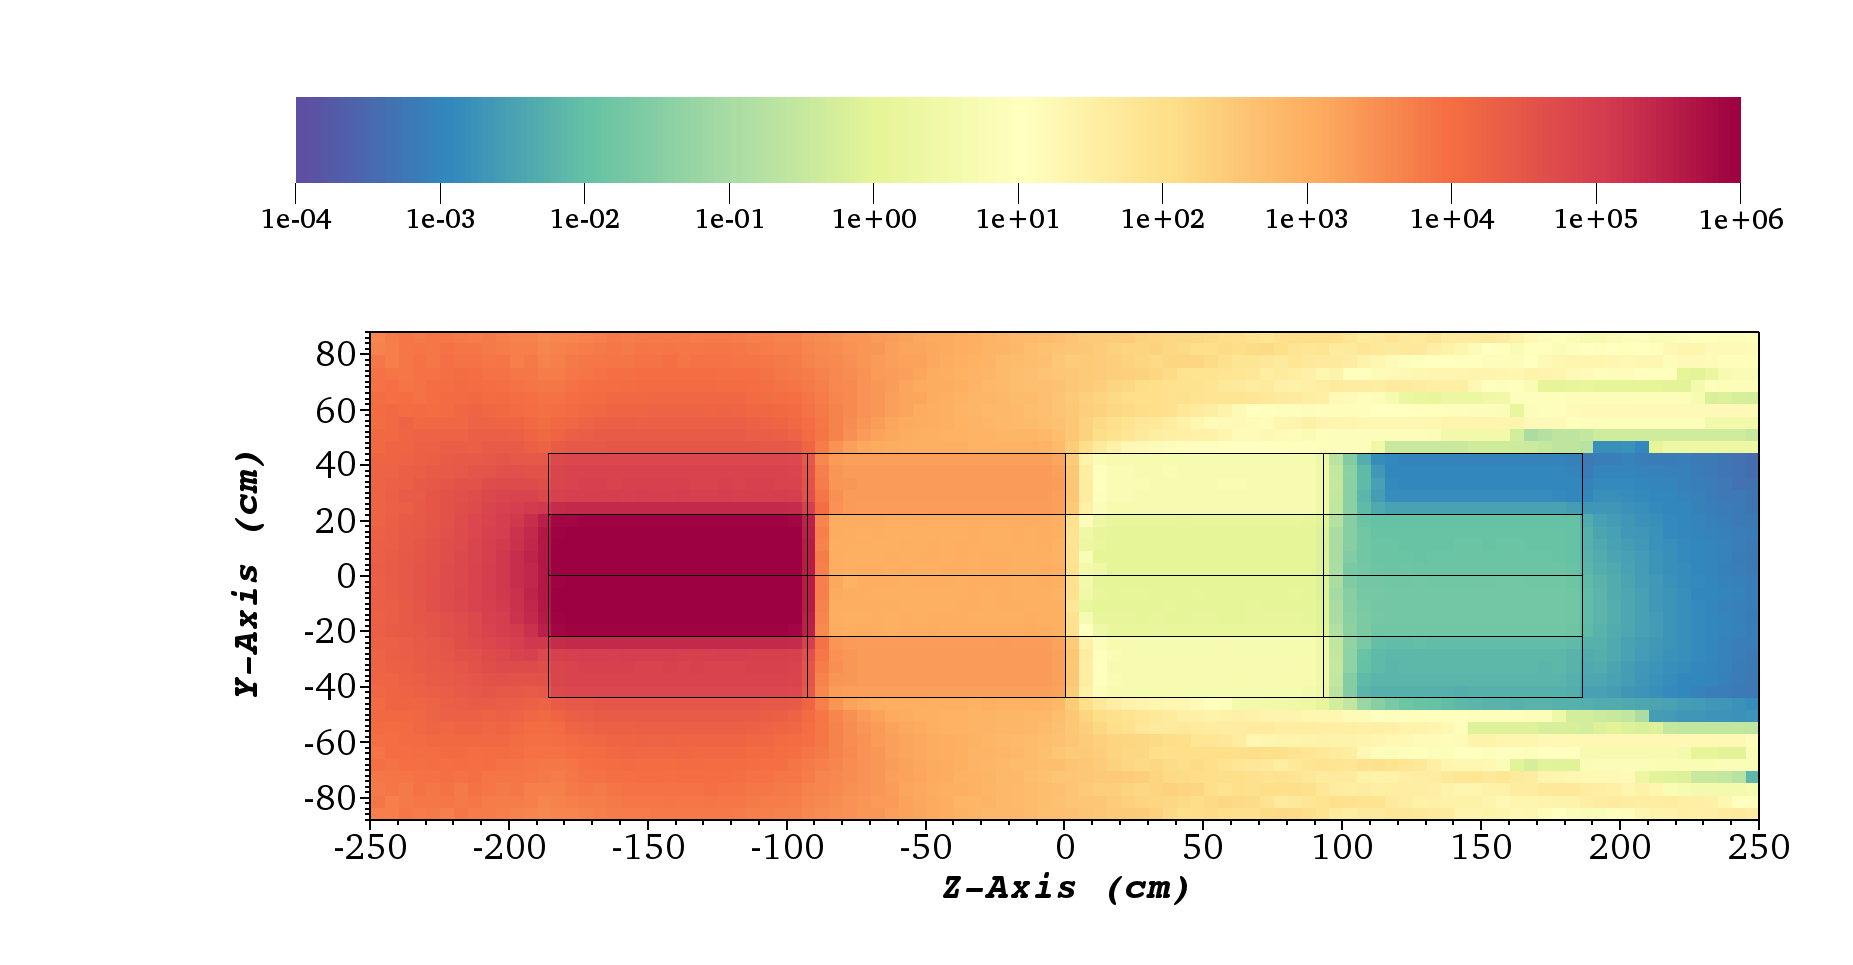
\includegraphics[width=\linewidth, trim={8cm 2cm 2cm 10cm},clip]{../figs/toy_p2/dose_VPII_4x_split.png}
		\caption{4x4x4 divided}
		\label{fig:2dose_4x_split}
	\end{subfigure}\hfill
	\begin{subfigure}[t]{0.5\textwidth}
		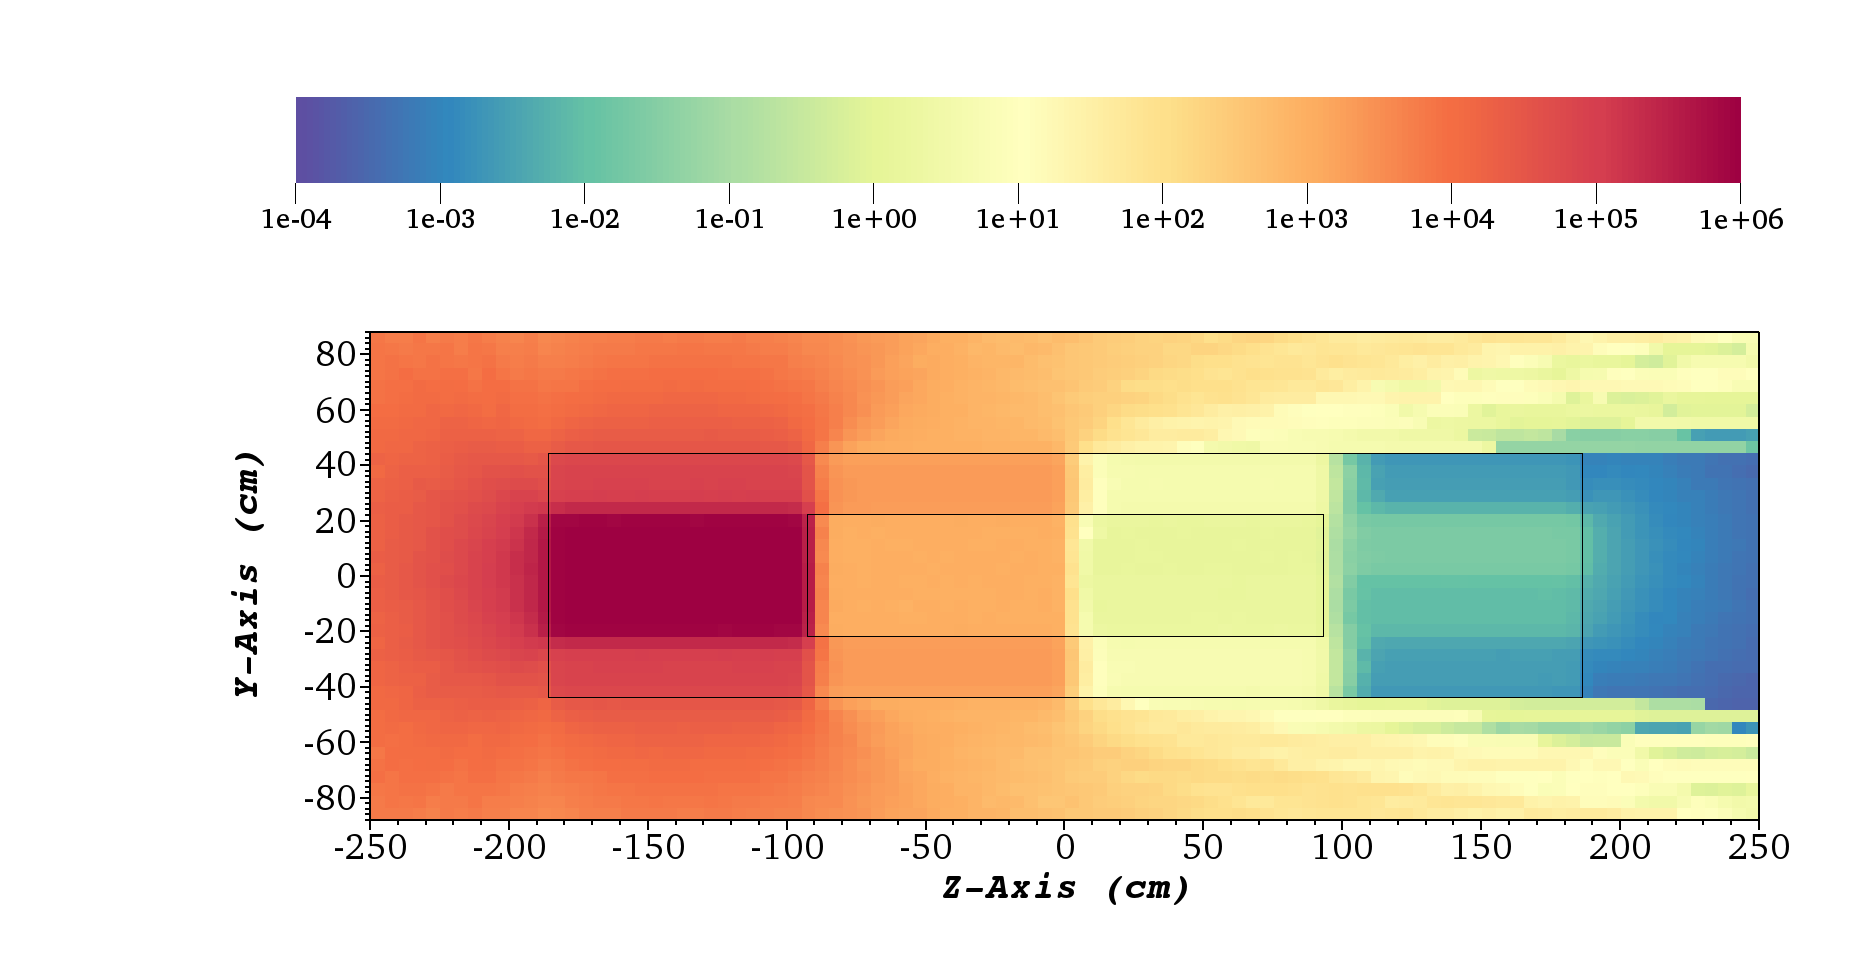
\includegraphics[width=\linewidth, trim={8cm 2cm 2cm 10cm},clip]{../figs/toy_p2/dose_VPII_4x_mesh.png}
		\caption{4x4x4 mesh}
		\label{fig:2dose_4x_mesh}
	\end{subfigure}

	\begin{subfigure}[t]{1.0\textwidth}
		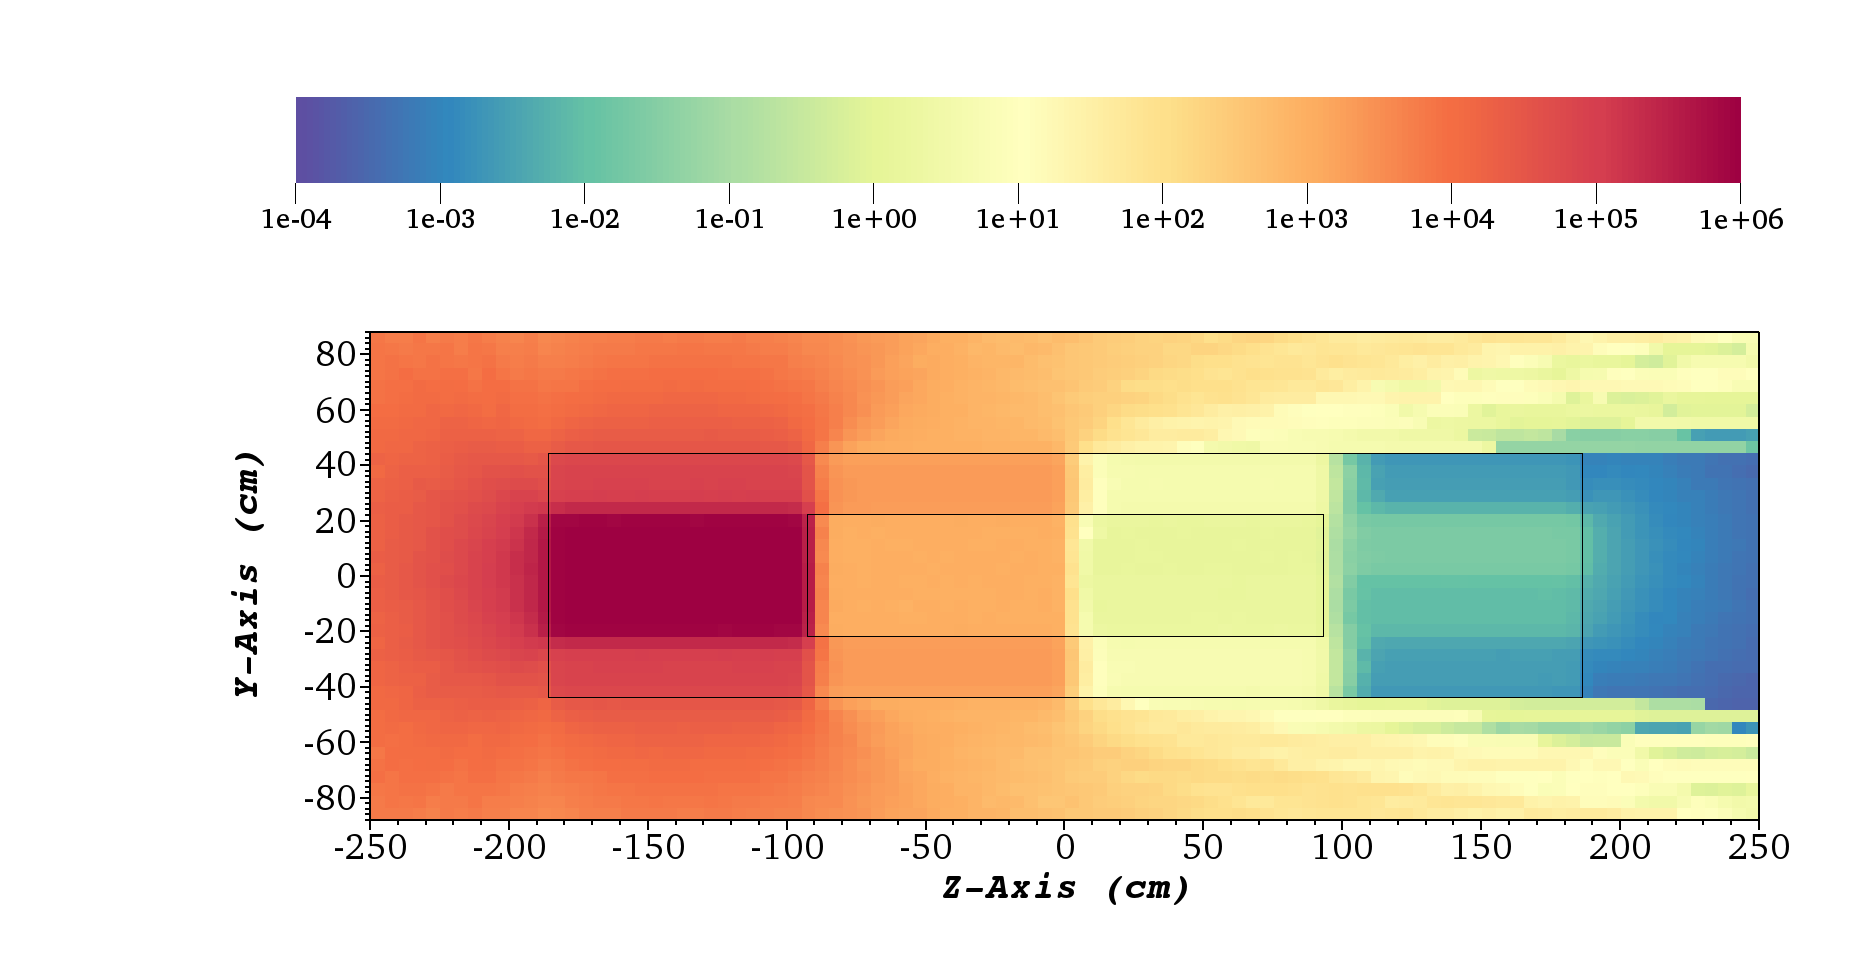
\includegraphics[width=\linewidth, trim={8cm 26cm 2cm 2cm},clip]{../figs/toy_p2/dose_VPII_4x_mesh.png}
		\label{fig:2legend}
	\end{subfigure}
	\caption{Biological dose rate on the mercury and steel cell with mesh and divided geometry}
	\label{fig:2dose}
\end{figure}
\\
A z score was done to compare between the results from the mesh workflow and the results
obtained with the cell based workflow. The results can be seen in Figure \ref{fig:}

\begin{figure}
	\begin{subfigure}[t]{0.5\textwidth}
		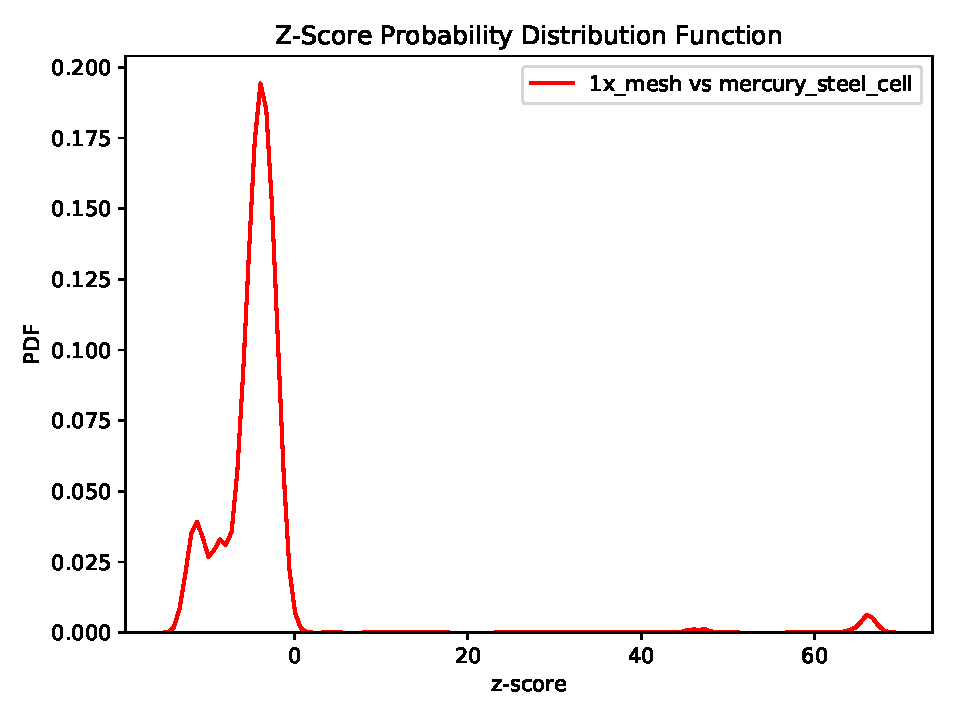
\includegraphics[width=\linewidth, trim={0cm 0cm 0cm 0.9cm},clip]{../figs/toy_p2/PDF_zscore_VPII_1x_orig.pdf}
		%\caption{PDF: 1x1x1x mesh to full geometry}
		\label{fig:2pdf_1x_orig}
	\end{subfigure}\hfill
	\begin{subfigure}[t]{0.5\textwidth}
		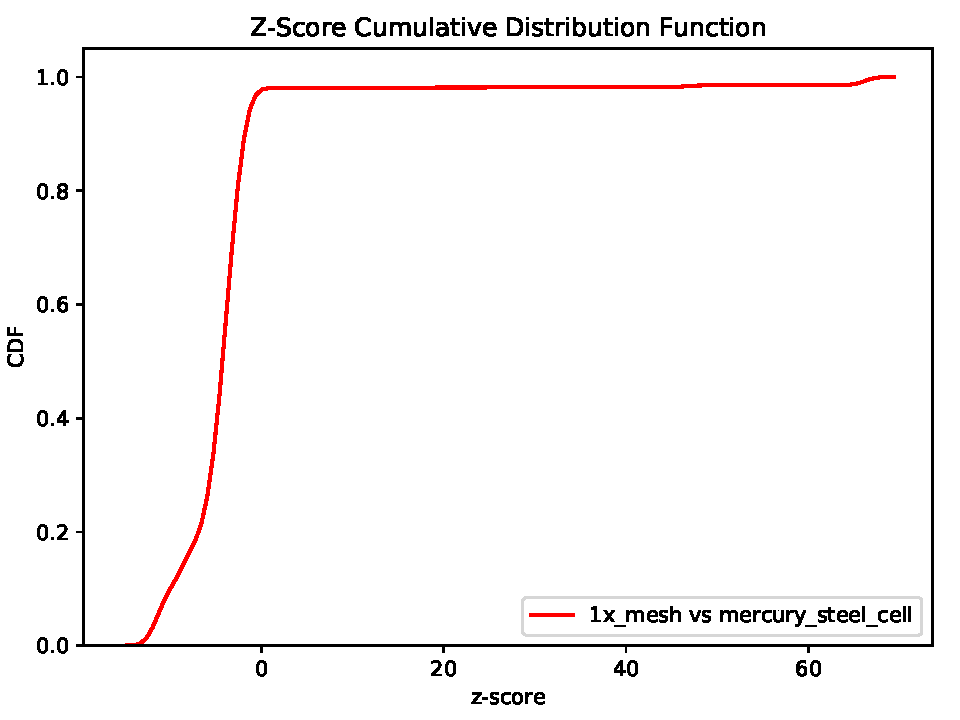
\includegraphics[width=\linewidth, trim={0cm 0cm 0cm 0.8cm},clip]{../figs/toy_p2/CDF_zscore_VPII_1x_orig.pdf}
		% \caption{CDF: 1x1x1 mesh to full geometry}
		\label{fig:2cdf_1x_orig}
	\end{subfigure}

	\begin{subfigure}[t]{0.5\textwidth}
		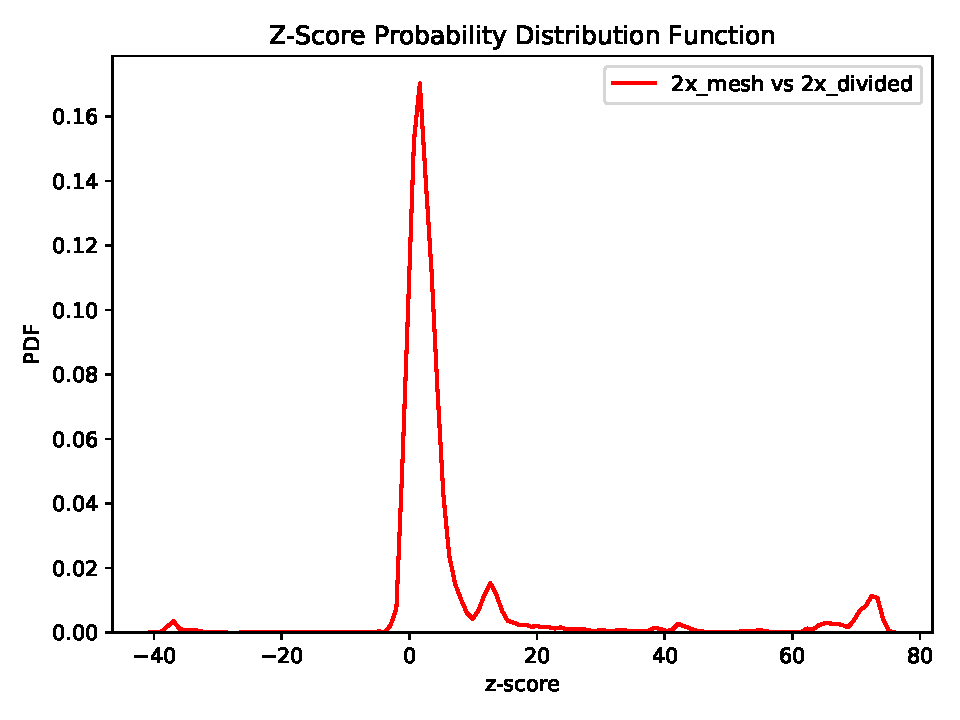
\includegraphics[width=\linewidth, trim={0cm 0cm 0cm 0.9cm},clip]{../figs/toy_p2/PDF_zscore_VPII_2xm_2xs.pdf}
		% \caption{2x2x2 divided}
		\label{fig:2dose_2x_split}
	\end{subfigure}\hfill
	\begin{subfigure}[t]{0.5\textwidth}
		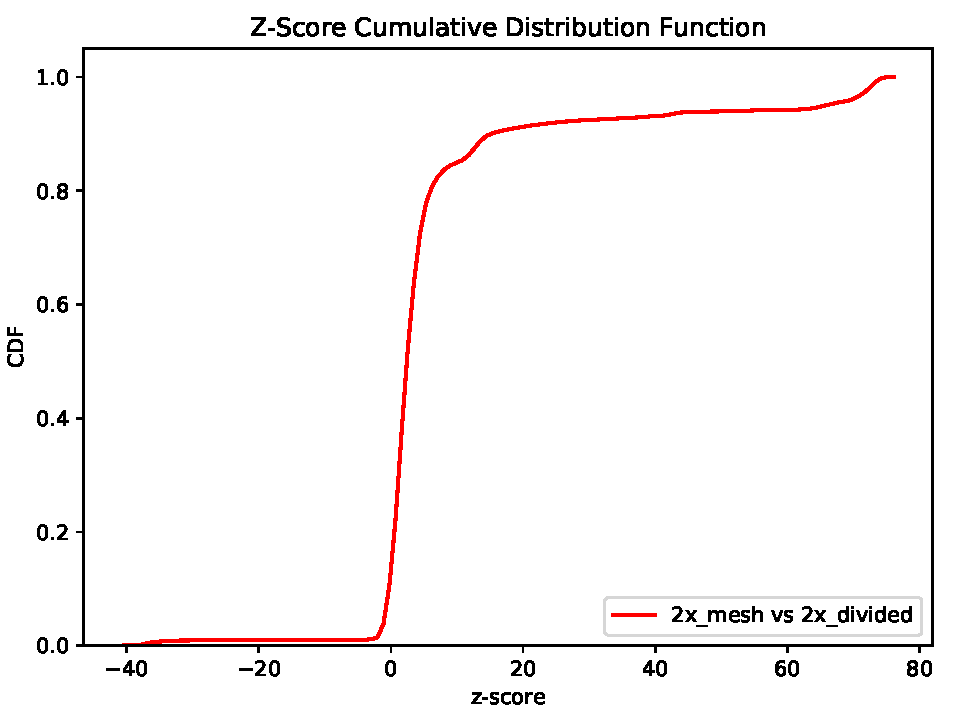
\includegraphics[width=\linewidth, trim={0cm 0cm 0cm 0.8cm},clip]{../figs/toy_p2/CDF_zscore_VPII_2xm_2xs.pdf}
		% \caption{2x2x2 mesh}
		\label{fig:2dose_2x_mesh}
	\end{subfigure}

	\begin{subfigure}[t]{0.5\textwidth}
		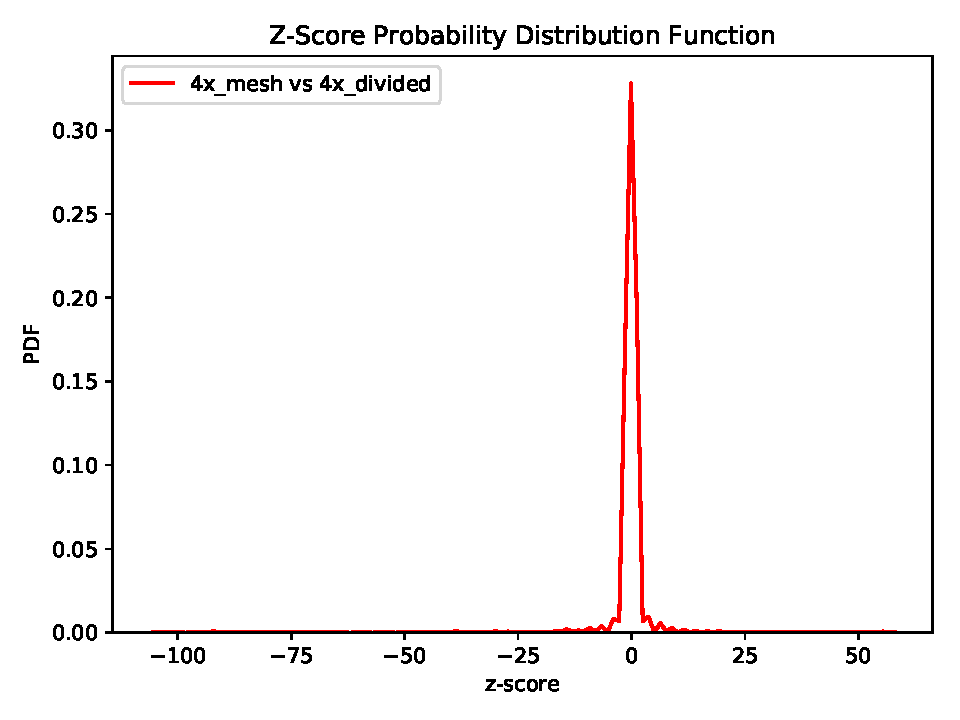
\includegraphics[width=\linewidth, trim={0cm 0cm 0cm 0.9cm},clip]{../figs/toy_p2/PDF_zscore_VPII_4xm_4xs.pdf}
		% \caption{4x4x4 divided}
		\label{fig:2dose_4x_split}
	\end{subfigure}\hfill
	\begin{subfigure}[t]{0.5\textwidth}
		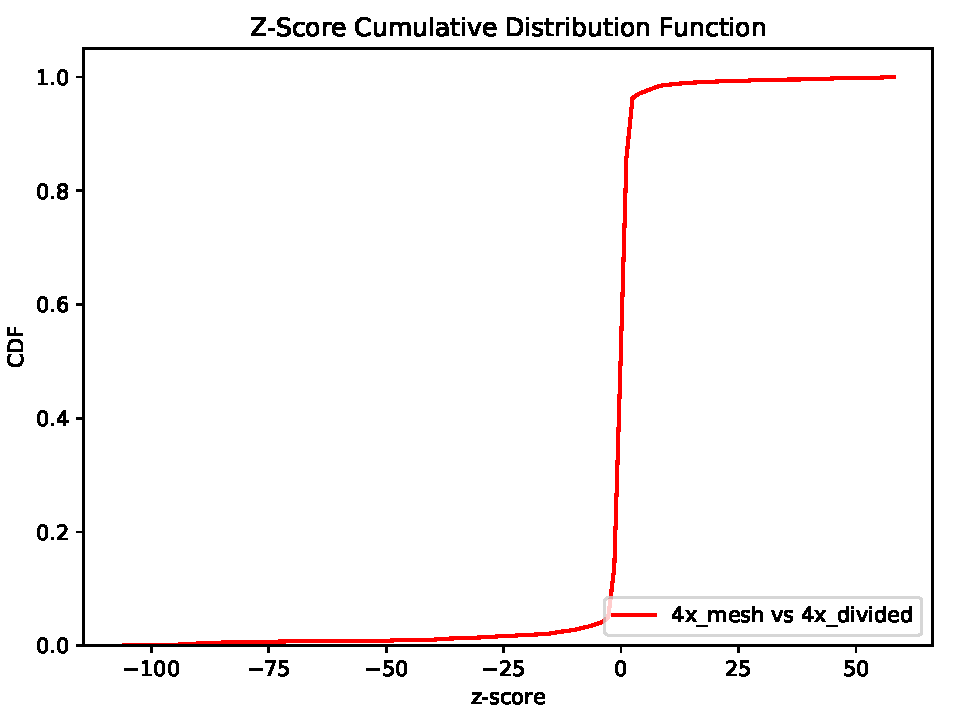
\includegraphics[width=\linewidth, trim={0cm 0cm 0cm 0.8cm},clip]{../figs/toy_p2/CDF_zscore_VPII_4xm_4xs.pdf}
		% \caption{4x4x4 mesh}
		\label{fig:2dose_4x_mesh}
	\end{subfigure}
	\caption{Z scores PDF and CDF comparing the results for the mesh to respective divided geometry }
	\label{fig:2z_score}
\end{figure}
\newpage
